%!TEX program = xelatex
\documentclass[11pt,a4paper]{article}
\usepackage[utf8]{inputenc}
\usepackage[T1]{fontenc}
\usepackage{authblk}
\usepackage{tikz}
\usepackage{pgfplots}
\usepackage{verbatim}
\usepackage{amsfonts}
\usepackage{amsmath}
\usepackage{amsthm}
\usepackage{enumerate}
\usepackage{indentfirst}
\usepackage{amssymb}
\linespread{1.6}\setlength{\footskip}{20pt}\setlength{\parindent}{0pt}
\usetikzlibrary{shapes,snakes}
\newcommand{\argmax}{\operatornamewithlimits{argmax}}
\newcommand{\argmin}{\operatornamewithlimits{argmin}}
\DeclareMathOperator{\col}{col}
\usepackage{booktabs}
\newtheorem{theorem}{Theorem}
\newtheorem{note}{Note}
\newtheorem{definition}{Definition}
\newtheorem{proposition}{Proposition}
\newtheorem{claim}{Claim}
\newtheorem{lemma}{Lemma}
\newtheorem{example}{Example}
\newtheorem{corollary}{Corollary}
\usepackage{graphicx}
\usepackage{geometry}
\usepackage{hyperref}
\newcommand{\code}{	exttt}
\geometry{a4paper,scale=0.8}
\title{Inference and Learning}
\author[*]{Wenxiao Yang}
\affil[*]{Department of Mathematics, University of Illinois at Urbana-Champaign}
\date{2022}
\begin{document}
\maketitle
\tableofcontents
\newpage

\section{Learning Basics}
\subsection{Parameters and Hyperparameters}
\begin{definition}
    \textbf{Parameters} are values learned by the model given the data.
\end{definition}
e.g. $\beta, W, b, \theta$.
\begin{definition}
    \textbf{Hyperparameters} are values supplied to tune the model and cannot be learned from data.
\end{definition}
e.g. Number of Hidden Layers, Neurons, and Epochs to Train. Learning Rate, and Batch Size.

\subsection{Neural Network: Back Propagation Algorithm}
\underline{\textbf{Neural Network}}
\begin{center}\begin{figure}[htbp]
    \centering
    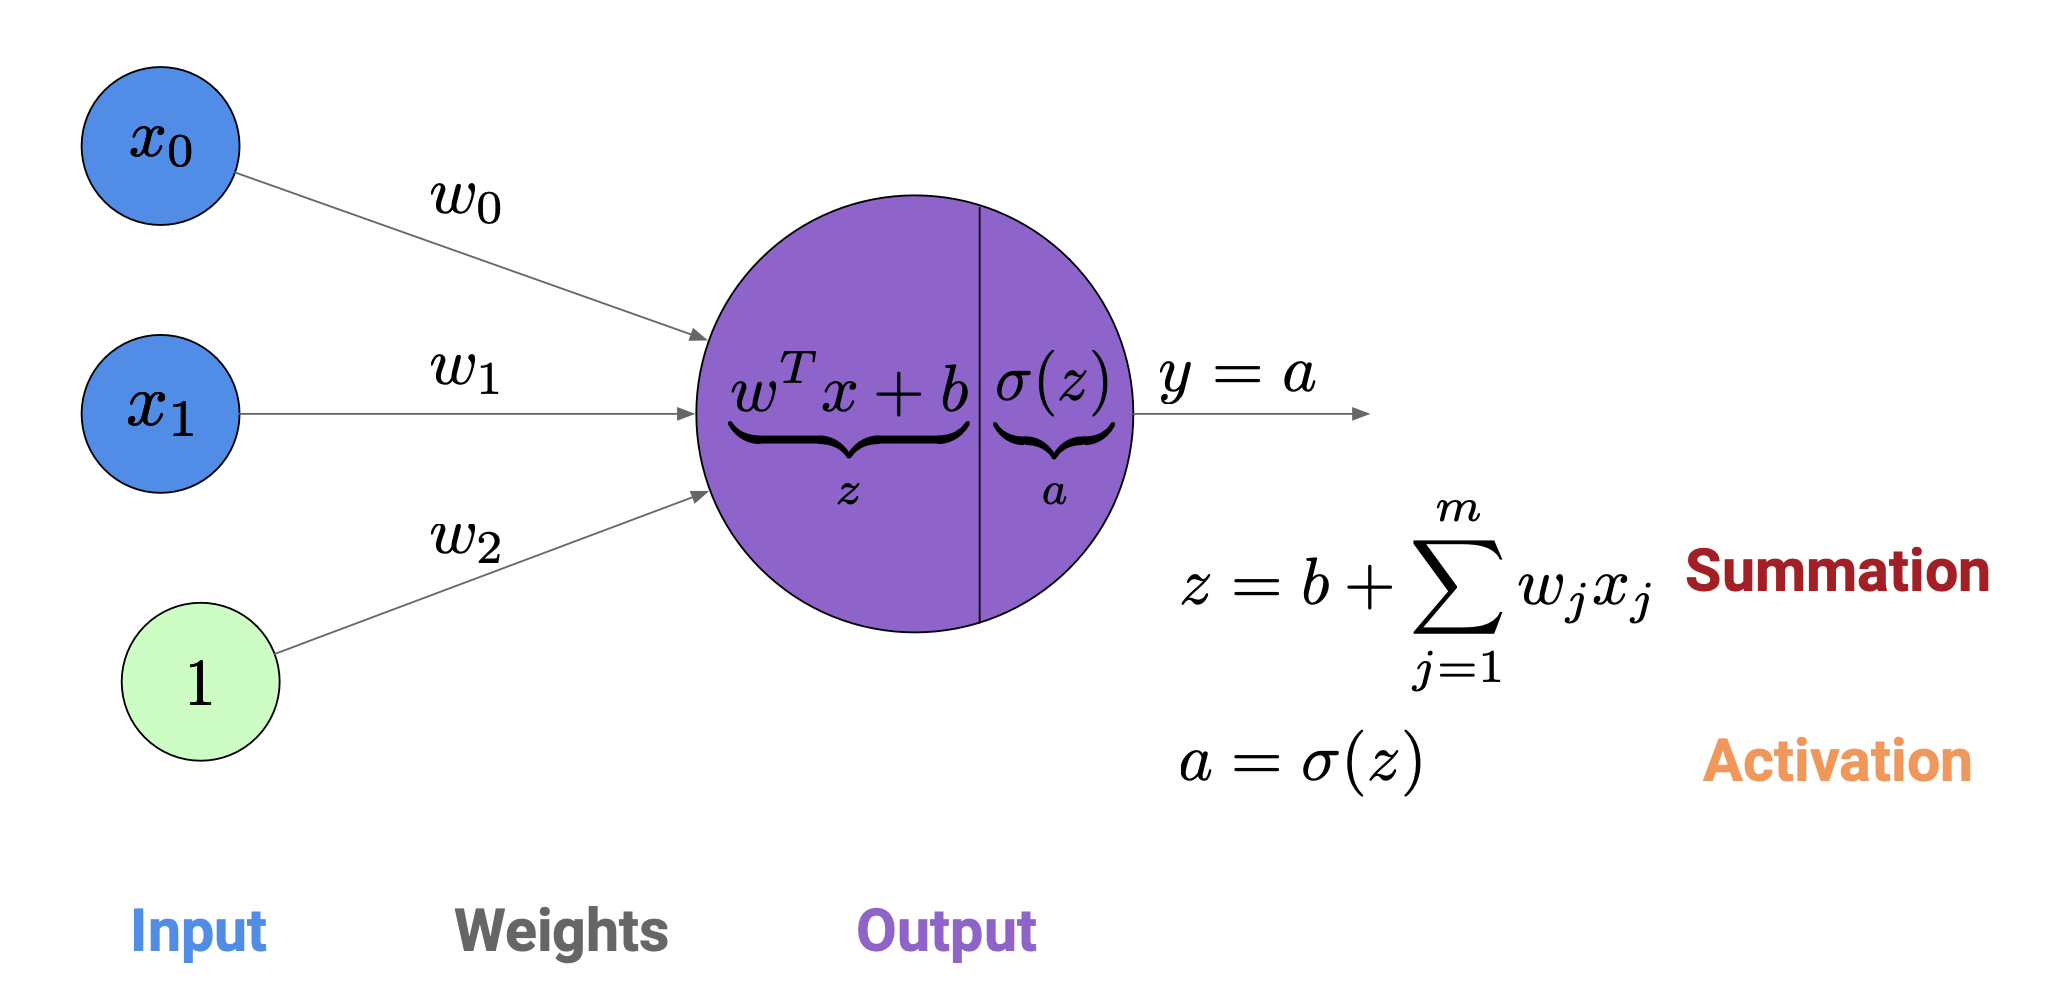
\includegraphics[scale=0.2]{neuron1.png}
    \caption{Simple Neural Network}
    \label{}
\end{figure}\end{center}
Given a vector input $x$, we need to find the best estimator $\hat{y}$ which minimizes lost function. In the figure that has only one layer and one pathway, we find the parameter $(\omega,b)$ to form an input $\omega^Tx+b$ to neuron $\sigma$ (activation function).  Then, the final output (estimator) of the network is $\hat{y}=\sigma(\omega^Tx+b)$.


\subsubsection{Activations}
\begin{definition}
    \underline{Activation functions} are element-wise gates for letting information propagate to future layers either transformed with non-linearities or left as-is.
\end{definition}
\textbf{Example of activation function:}
\begin{center}\begin{figure}[htbp]
    \centering
    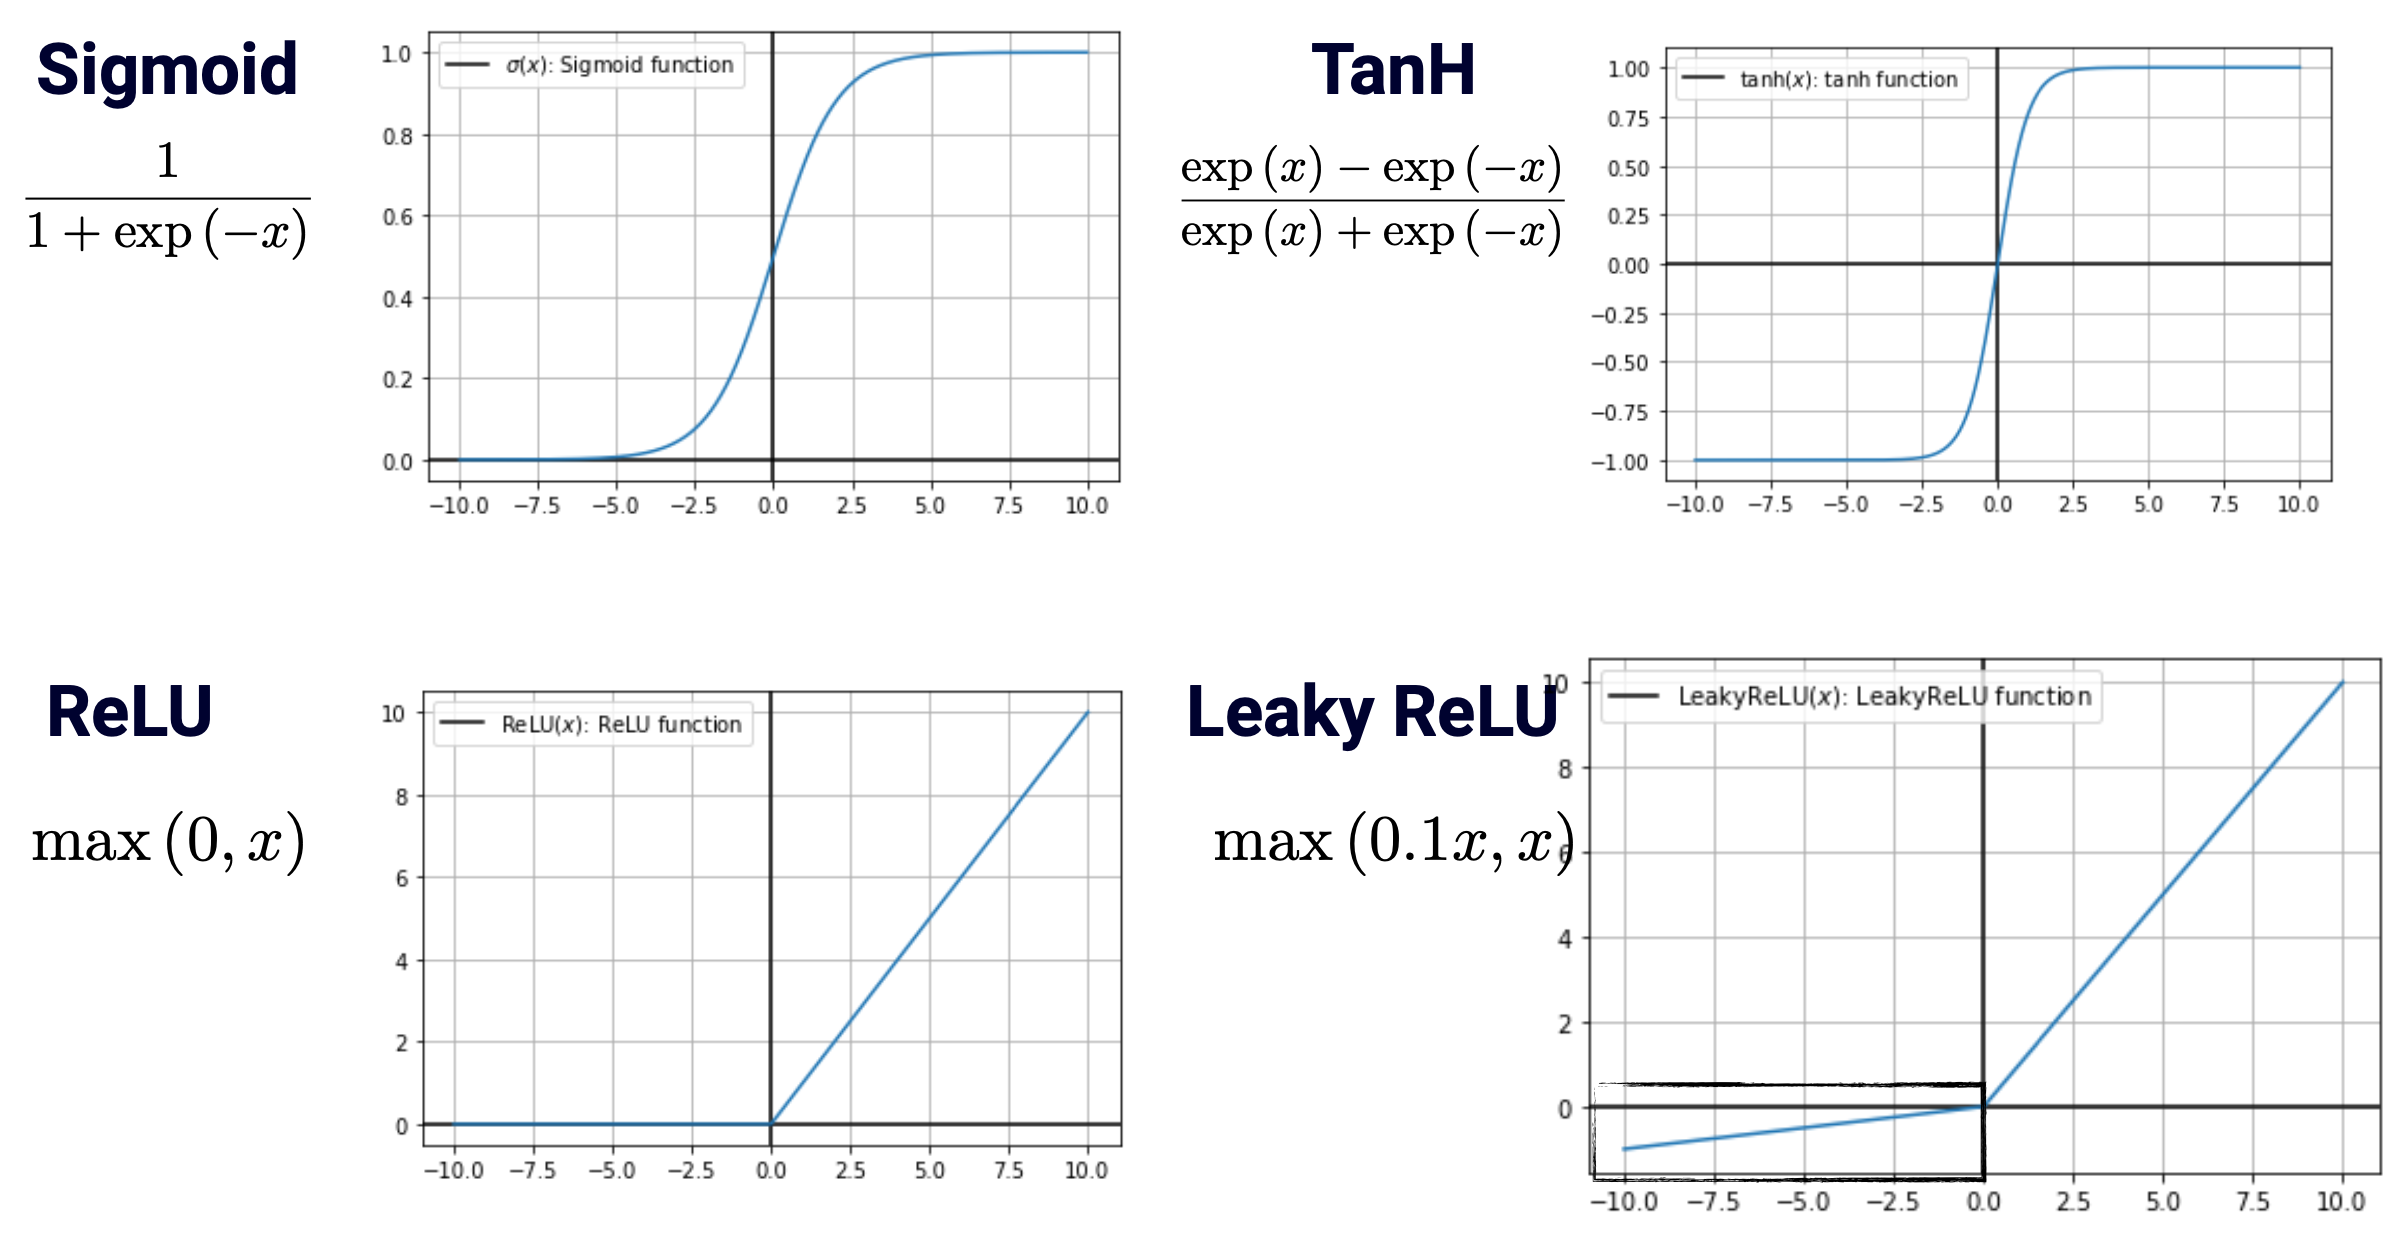
\includegraphics[scale=0.2]{activations.png}
    \caption{Activations}
    \label{}
\end{figure}\end{center}
\begin{enumerate}[(1)]
    \item \textbf{Identity:} $$\text{identity}(x)=I(x)=x$$
    \item \textbf{Binary:} $$\text{binary}(x)=\text{step}(x)=\left\{\begin{matrix}
        1,&x\geq 0\\
        0,&x<0
    \end{matrix}\right.$$
    \item \textbf{Sigmoid:}$$\sigma(x)=\frac{1}{e^{-x}}$$
    \begin{equation}
        \begin{aligned}
            \sigma(-x)=1-\sigma(x);\
            \frac{d\sigma(x)}{dx}=\sigma(x)\cdot(1-\sigma(x))
        \end{aligned}
        \nonumber
    \end{equation}
    \begin{equation}
        \begin{aligned}
            \frac{\partial \sigma(\vec{x})}{\partial \vec{x}}=\begin{bmatrix}
                \sigma(x_1)(1-\sigma(x_1)) &\cdots&0\\
                \vdots&\ddots&\vdots\\
                0&\cdots&\sigma(x_n)(1-\sigma(x_n))
            \end{bmatrix}=\text{diag}(\sigma(\vec{x})\cdot (1-\sigma(\vec{x})))
        \end{aligned}
        \nonumber
    \end{equation}
    \item \textbf{TanH:} $$tanh(x)=\frac{e^x-e^{-x}}{e^x+e^{-x}}$$(TanH is a rescaled sigmoid) $$tanh(x)=\frac{e^{2x}-1}{e^{2x}+1}=1-2\sigma(-2x)=2\sigma(2x)-1$$
    \item \textbf{ReLU:} $$g(x)=\max(0,x)$$
    \item \textbf{Leaky ReLU:} $$g(x)=\max(0.1x,x)$$
    \item \textbf{Softmax:} $S_j(\vec{x})=\frac{e^{x_j}}{\sum_{i=1}^ne^{x_i}}$, $$S(\vec{x})=\left[\frac{e^{x_1}}{\sum_{i=1}^ne^{x_i}},\frac{e^{x_2}}{\sum_{i=1}^ne^{x_i}},\cdots, \frac{e^{x_n}}{\sum_{i=1}^ne^{x_i}}\right]^T$$
    $$\frac{\partial S_j(\vec{x})}{\partial x_j}=S_j(\vec{x})[1-S_j(\vec{x})]$$
\end{enumerate}


\subsubsection{Multilayer Neural Network}
\begin{center}\begin{figure}[htbp]
    \centering
    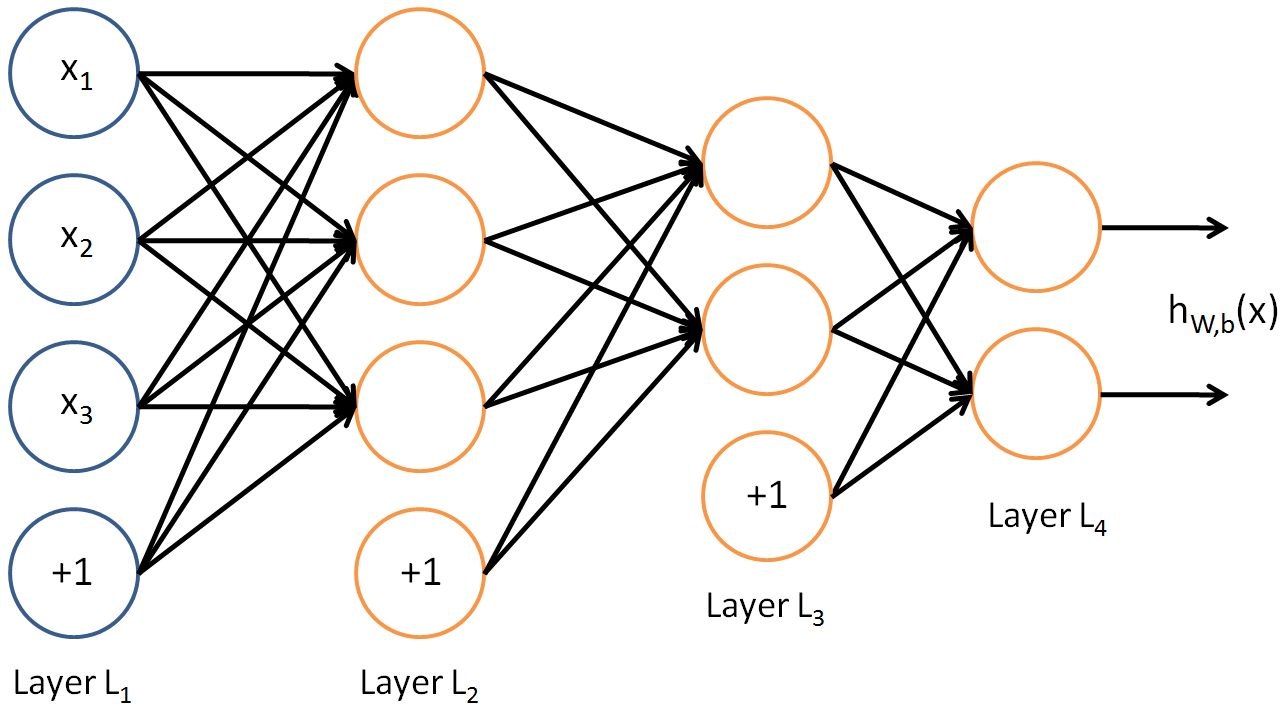
\includegraphics[scale=0.2]{MNN.png}
    \caption{Multilayer Neural Network}
    \label{}
\end{figure}\end{center}
\begin{enumerate}[$\bullet$]
    \item Number of neurons in each layer can be different.
    \item All weights on edge connecting layers $m-1$ and $m$ is matrix $W^{(m)}$, with $w_{ij}^{(m)}$ being the weight connecting output $j$ of layer $m-1$ with neuron $i$ of layer $m$.
    \item Input to network is vector $x$; output of layer $m$ is vector $y^{(m)}$
    \begin{equation}
        \begin{aligned}
            y_i^{(1)}=\sigma(x_i^{(1)}),&\text{ with }x_i^{(1)}=\sum_jw_{ij}^{(1)}x_j+b_i^{(1)}\\
            y^{(1)}=\sigma(x^{(1)}),&\text{ with }x^{(1)}=W^{(1)}x+b^{(1)}\\
            y^{(2)}=\sigma(x^{(2)}),&\text{ with }x^{(2)}=W^{(2)}y^{(1)}+b^{(2)}\\
            \vdots&\\
            y^{(M)}=\sigma(x^{(M)}),&\text{ with }x^{(M)}=W^{(M)}y^{(M-1)}+b^{(M)}\\
        \end{aligned}
        \nonumber
    \end{equation}
\end{enumerate}

We want to find the weights $W^{(1)},\cdots,W^{(M)},b^{(1)},\cdots,b^{(M)}$ so that the output of last layer
\begin{equation}
    \begin{aligned}
        \hat{y}=y^{(M)}\approx f^*(x)=y
    \end{aligned}
    \nonumber
\end{equation}
$f^*(x)$ is the unknown thing we need to predict.

We use \underline{labelled training data}, i.e.
\begin{equation}
    \begin{aligned}
        (x[1],y[1]),(x[2],y[2]),\cdots (x[N],y[N])
    \end{aligned}
    \nonumber
\end{equation}
Minimize the "empirical" loss on training data.
\begin{equation}
    \begin{aligned}
        J=\sum_{i=1}^N L(y[i],\hat{y}[i])
    \end{aligned}
    \nonumber
\end{equation}
where $\bar{y}[i]$ is the output of NN whose input is $x[i]$.

\begin{enumerate}[$\bullet$]
    \item $L$ is the function of $W^{(1)},\cdots,W^{(M)},b^{(1)},\cdots,b^{(M)}$ to measure the loss. e.g. the square loss $$L(y,\hat{y})=(y-\hat{y})^2$$
    \item We wish to minimize $J$ using a \underline{gradient descent procedure}.
    \item To compute gradient we need:
    \begin{equation}
        \begin{aligned}
            \frac{\partial L}{\partial w_{ij}^{(l)}}\text{ for each }l,i,j; \quad
            \frac{\partial L}{\partial b_i^{(l)}}\text{ for each }l,i.\\
        \end{aligned}
        \nonumber
    \end{equation}
\end{enumerate}

\subsubsection{A Simple Example of Back Propagation Algorithm}
We can consider a simple example (one layer, two pathways)
\begin{center}\begin{figure}[htbp]
    \centering
    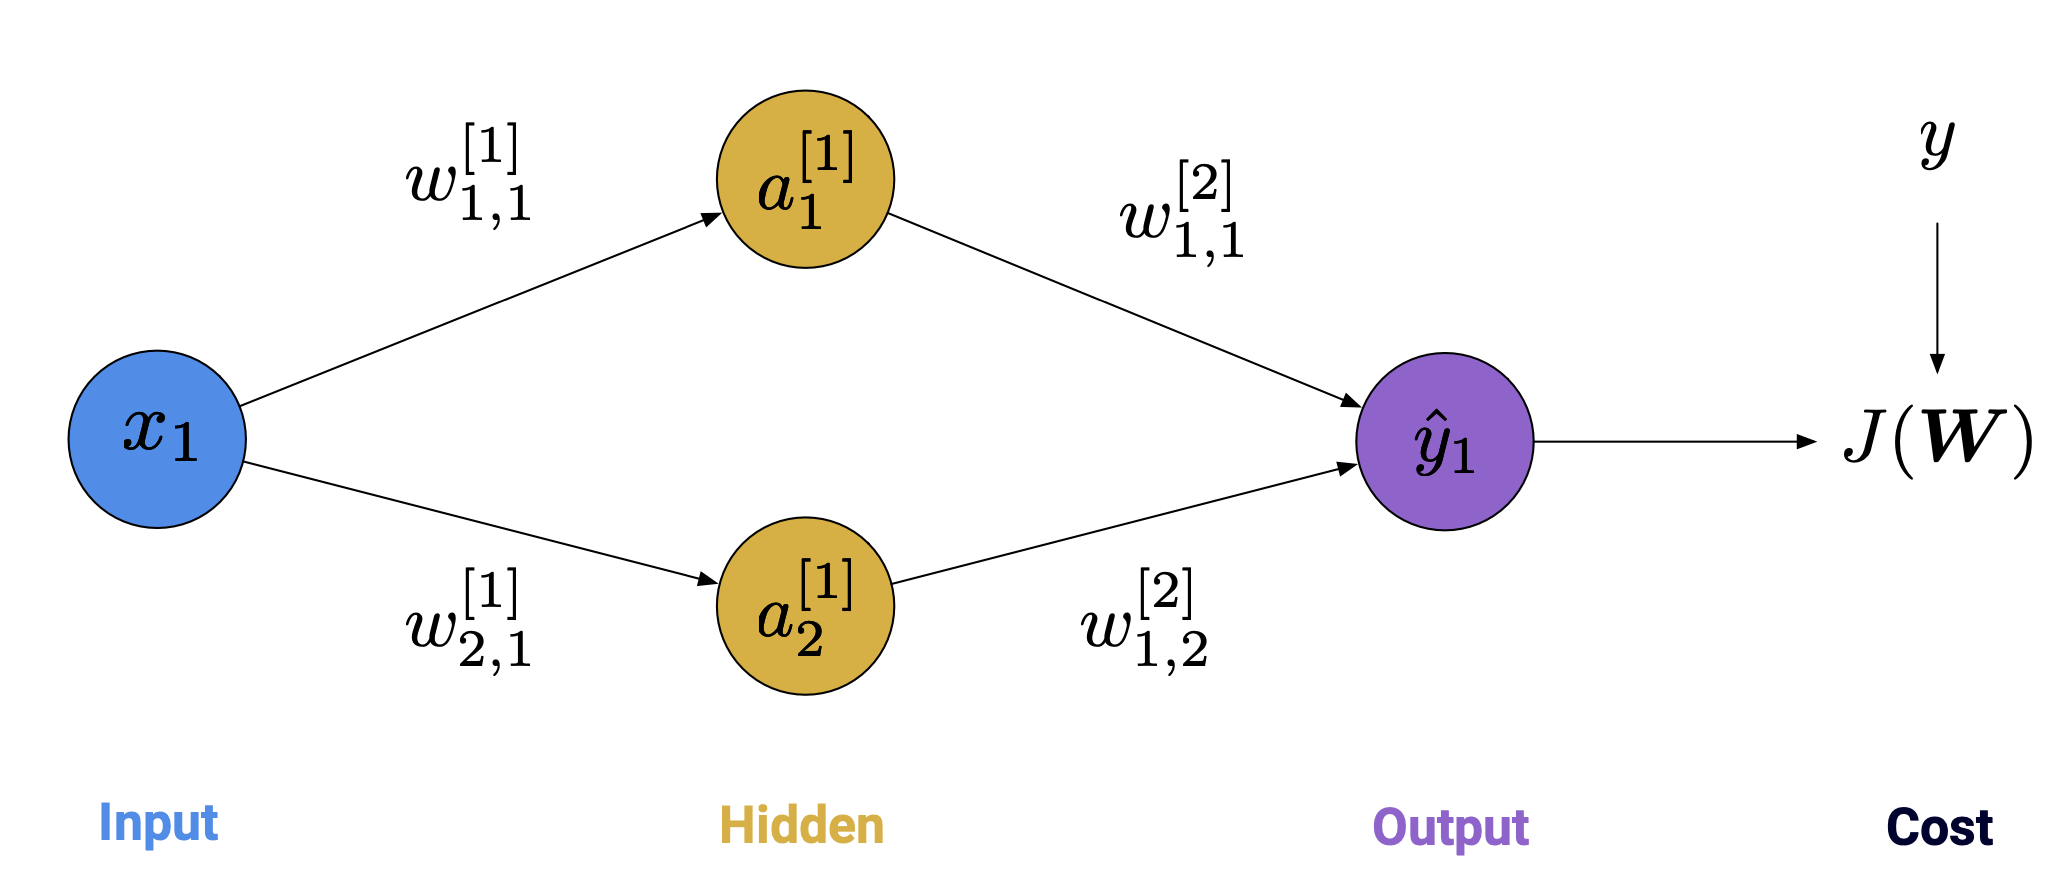
\includegraphics[scale=0.2]{2path.png}
    \caption{Two Independent Pathways}
    \label{}
\end{figure}\end{center}
$W^{(1)}=[w_{1,1}^{[1]},w_{2,1}^{[1]}]^T$, $b^{(1)}=[0,0]^T$, $\sigma_1(x)=x$.

$W^{(2)}=[w_{1,1}^{[2]},w_{1,2}^{[2]}]$, $b^{(2)}=0$, $\sigma_2(x)=x$.

\begin{equation}
    \begin{aligned}
        [a_1^{[1]},a_2^{[1]}]^T&=\sigma_1(W^{(1)}x_1+b^{(1)})=[w_{1,1}^{[1]}x_1,w_{2,1}^{[1]}x_1]^T\\
        \hat{y}&=\sigma_2(W^{(2)}[a_1^{[1]},a_2^{[1]}]^T+b^{(2)})=(w_{1,1}^{[1]}w_{1,1}^{[2]}+w_{2,1}^{[1]}w_{1,2}^{[2]})x_1
    \end{aligned}
    \nonumber
\end{equation}

\begin{equation}
    \begin{aligned}
        \frac{\partial J(\hat{y})}{\partial w_{2,1}^{[1]}}=\frac{\partial J(\hat{y})}{\partial \hat{y}}\cdot \frac{\hat{y}}{\partial a_2^{[1]}}\cdot\frac{a_2^{[1]}}{\partial w_{2,1}^{[1]}}
    \end{aligned}
    \nonumber
\end{equation}

\subsubsection{Back Propagation Algorithm}
Recall $y_i^{(m)}=\sigma(x_i^{(m)})$, $x_i^{(m)}=\sum_jw_{ij}^{(m)}y_j^{(m-1)}+b_i^{(m)}$
\begin{equation}
    \begin{aligned}
        \frac{\partial L}{\partial w_{ij}^{(m)}}=\frac{\partial L}{\partial y_i^{(m)}}\cdot \frac{\partial y_i^{(m)}}{\partial w_{ij}^{(m)}}=\frac{\partial L}{\partial y_i^{(m)}}\cdot \frac{\partial y_i^{(m)}}{\partial x_{i}^{(m)}}\cdot \frac{\partial x_{i}^{(m)}}{\partial w_{ij}^{(m)}}
    \end{aligned}
    \nonumber
\end{equation}
\begin{equation}
    \begin{aligned}
        \frac{\partial L}{\partial b_{i}^{(m)}}&=\frac{\partial L}{\partial y_i^{(m)}}\cdot \frac{\partial y_i^{(m)}}{\partial x_{i}^{(m)}}\cdot \frac{\partial x_{i}^{(m)}}{\partial b_{i}^{(m)}}\\
    \end{aligned}
    \nonumber
\end{equation}

\textbf{\underline{For large $M$}},
\begin{enumerate}[$\bullet$]
    \item $\frac{\partial L}{\partial y_i^{(M)}}$ is easy to compute.
    \item $\frac{\partial y_i^{(M)}}{\partial x_{i}^{(M)}}=\frac{\partial \sigma(x_{i}^{(M)})}{\partial x_{i}^{(M)}}=\sigma'(x_{i}^{(M)})$, (assuming $\sigma$ differentiable).
    \item $\frac{\partial x_{i}^{(M)}}{\partial w_{ij}^{(M)}}=y_j^{(M-1)}$
\end{enumerate}
Thus,
\begin{equation}
    \begin{aligned}
        \frac{\partial L}{\partial w_{ij}^{(M)}}=\frac{\partial L}{\partial y_i^{(M)}}\cdot \sigma'(x_{i}^{(M)}) \cdot y_j^{(M-1)}
    \end{aligned}
    \nonumber
\end{equation}
Similarly,
\begin{equation}
    \begin{aligned}
        \frac{\partial L}{\partial b_{i}^{(M)}}&=\frac{\partial L}{\partial y_i^{(M)}}\cdot \frac{\partial y_i^{(M)}}{\partial x_{i}^{(M)}}\cdot \frac{\partial x_{i}^{(M)}}{\partial b_{i}^{(M)}}\\
        &=\frac{\partial L}{\partial y_i^{(M)}}\cdot \sigma'(x_{i}^{(M)})
    \end{aligned}
    \nonumber
\end{equation}

\textbf{\underline{For $1\leq m< M$}}, in this situation $\frac{\partial L}{\partial y_i^{(m)}}$ is not easy to compute. Note that $x^{(m+1)}=W^{(m+1)}y^{(m)}+b^{(m+1)}$.
\begin{equation}
    \begin{aligned}
    \frac{\partial L}{\partial y_i^{(m)}}&=\sum_k \frac{\partial L}{\partial x_{k}^{(m+1)}}\cdot \frac{\partial x_{k}^{(m+1)}}{\partial y_i^{(m)}}\\
    &=\sum_k \frac{\partial L}{\partial y_{k}^{(m+1)}}\cdot\frac{\partial y_{k}^{(m+1)}}{\partial x_{k}^{(m+1)}}\cdot \frac{\partial x_{k}^{(m+1)}}{\partial y_i^{(m)}}\\
    &=\sum_k \frac{\partial L}{\partial y_{k}^{(m+1)}}\cdot\sigma'(x_k^{(m+1)})\cdot w_{ki}^{(m+1)}\\
    \end{aligned}
    \nonumber
\end{equation}

Then use this form to compute,

(We can set $\delta^{(m)}=\frac{\partial L}{\partial y_i^{(m)}}\cdot \sigma'(x_{i}^{(m)})$ to avoid duplicate computation.)
\begin{equation}
    \begin{aligned}
        \frac{\partial L}{\partial w_{ij}^{(m)}}&=\frac{\partial L}{\partial y_i^{(m)}}\cdot \frac{\partial y_i^{(m)}}{\partial x_{i}^{(m)}}\cdot \frac{\partial x_{i}^{(m)}}{\partial w_{ij}^{(m)}}\\
        &=\frac{\partial L}{\partial y_i^{(m)}}\cdot \sigma'(x_{i}^{(m)}) \cdot y_j^{(m-1)}\\
        &=\delta^{(m)}\cdot y_j^{(m-1)}
    \end{aligned}
    \nonumber
\end{equation}

Similarly,
\begin{equation}
    \begin{aligned}
        \frac{\partial L}{\partial b_{i}^{(m)}}&=\frac{\partial L}{\partial y_i^{(m)}}\cdot \frac{\partial y_i^{(m)}}{\partial x_{i}^{(m)}}\cdot \frac{\partial x_{i}^{(m)}}{\partial b_{i}^{(m)}}\\
        &=\frac{\partial L}{\partial y_i^{(m)}}\cdot \sigma'(x_{i}^{(m)})\\
        &=\delta^{(m)}
    \end{aligned}
    \nonumber
\end{equation}

\begin{center}
    \fcolorbox{black}{gray!10}{\parbox{.9\linewidth}{
\textbf{Summary}
\begin{enumerate}
    \item Compute $\frac{\partial L}{\partial y_i^{(M)}}$.
    \item Use $$\frac{\partial L}{\partial y_i^{(m)}}=\sum_k \frac{\partial L}{\partial y_{k}^{(m+1)}}\cdot\sigma'(x_k^{(m+1)})\cdot w_{ki}^{(m+1)}$$ compute $\frac{\partial L}{\partial y_i^{(m)}}$ for $m=1,2...,M-1$.
    \item Compute $$\frac{\partial L}{\partial b_{i}^{(m)}}=\frac{\partial L}{\partial y_i^{(m)}}\cdot \sigma'(x_{i}^{(m)})=\delta^{(m)}$$ for $m=1,2...,M$.
    \item Compute $$\frac{\partial L}{\partial w_{ij}^{(m)}}=\frac{\partial L}{\partial y_i^{(m)}}\cdot \sigma'(x_{i}^{(m)}) \cdot y_j^{(m-1)}=\delta^{(m)}\cdot y_j^{(m-1)}$$ for $m=1,2...,M$.
\end{enumerate}
    }}
\end{center}

\subsubsection{Other Methods}
Stochastic Gradient Descent (SGD)

Subgradient Method

\subsection{Perceptron Algorithm}
\begin{definition}
    \underline{Binary linear classifiers} distinguish between two categories through a linear function of the inputs.
\end{definition}

\begin{definition}
    \underline{Linearly separable} refers to a line that can be drawn to perfectly split the two classes.
\end{definition}

The Perceptron algorithm is an efficient algorithm for learning a \textbf{linear separator} in $d-$dimensional space, with a mistake bound that depends on the margin of separation of the data.
\subsubsection{General Idea}
Given the training data $$D=\left\{\left\langle x^{(i)},y^{(i)}\right\rangle,i=1,...,n\right\}\in \left(\mathbb{R}^m\times\{0,1\}\right)^n$$ we want to know the exact value of $y\in\{0,1\}$.
\begin{center}\begin{figure}[htbp]
    \centering
    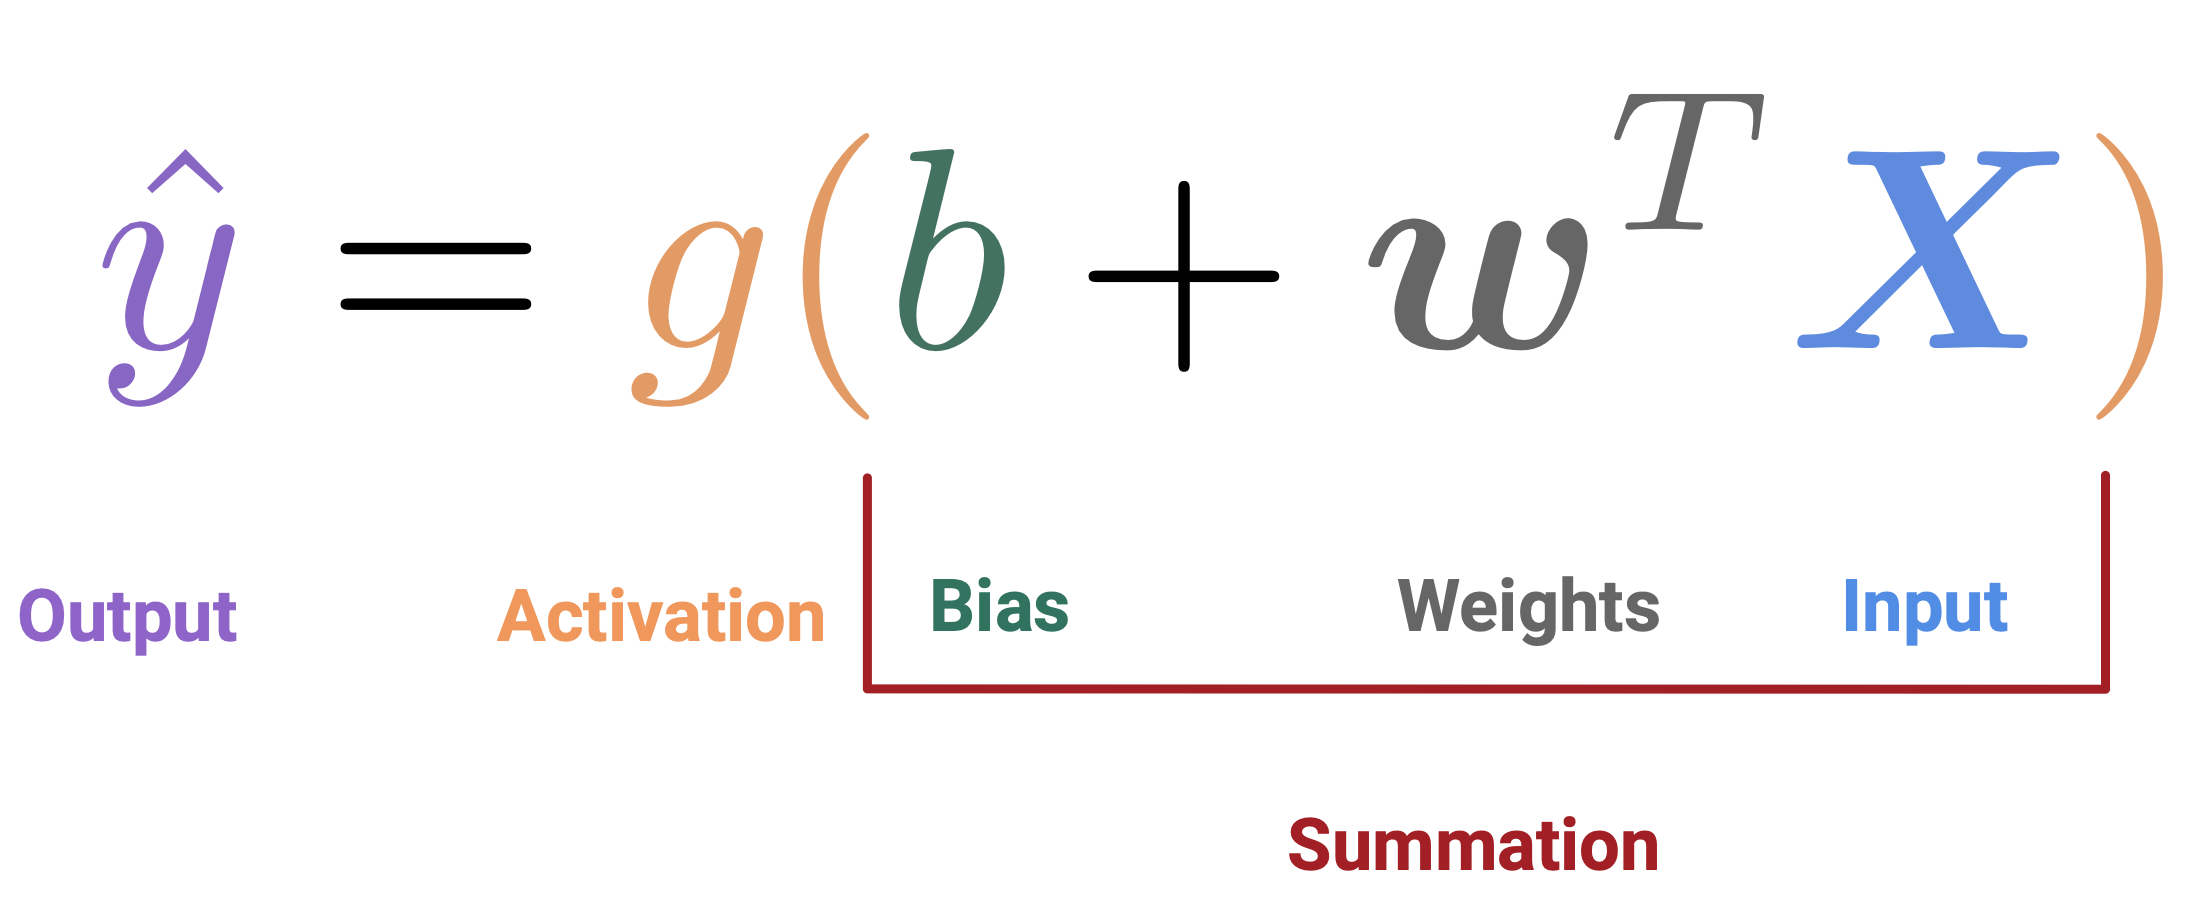
\includegraphics[scale=0.1]{Per_output.png}
    \caption{Perceptron Output}
    \label{}
\end{figure}\end{center}
\begin{center}
    \fcolorbox{black}{gray!10}{\parbox{.9\linewidth}{
    \subsubsection*{General idea:}
    \begin{enumerate}[$\bullet$]
        \item If the perceptron correctly predicts ($\hat{y}=y$):
        \begin{enumerate}[$\cdot$]
            \item Do nothing
        \end{enumerate}
        \item If the perceptron yields an incorrect prediction ($\hat{y}\neq y$):
        \begin{enumerate}[$\cdot$]
            \item If the prediction is $0$ and truth is $1$ ($\hat{y}=0|y=1 \Rightarrow e=y-\hat{y}=1$), add feature vector to weight vector.
            \item If the prediction is $1$ and truth is $0$ ($\hat{y}=1|y=0 \Rightarrow e=y-\hat{y}=-1$), subtract feature vector from the weight vector.
        \end{enumerate}
    \end{enumerate}
    }}
\end{center}

\begin{center}\begin{figure}[htbp]
    \centering
    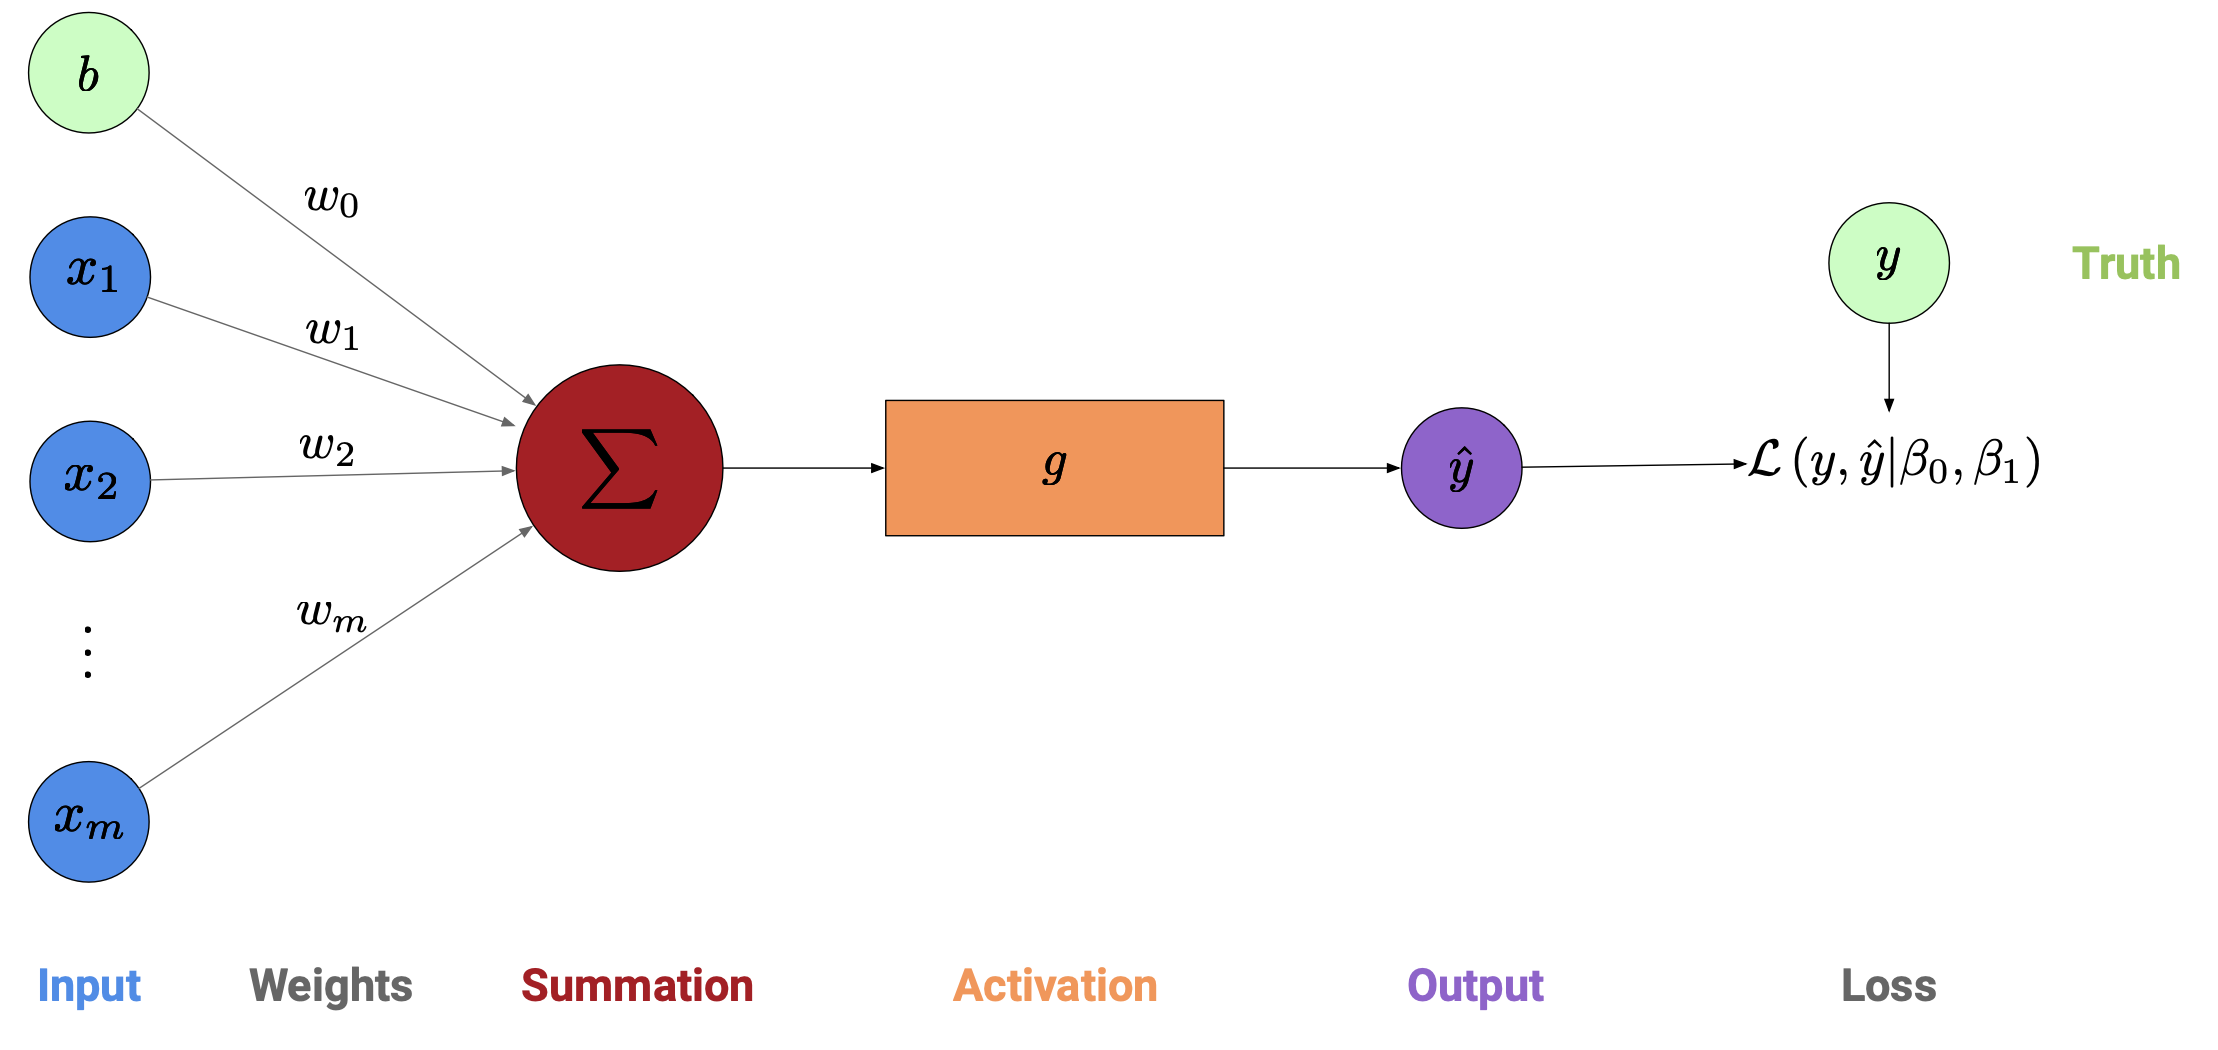
\includegraphics[scale=0.2]{per.png}
    \caption{Perceptron}
    \label{}
\end{figure}\end{center}

Since we want the prediction to be either $0$ or $1$, we usually use binary function as the activation function in perceptron.


\subsubsection{Algorithm}
\textbf{Perceptron Algorithm:}
\begin{enumerate}[$\bullet$]
    \item Initialize weights (including a bias term) to zero, e.g. $W=[w,b]=0^{m+1}$.
    \item Under each training epoch: Compute for each sample $\left\langle x^{(i)},y^{(i)}\right\rangle\in D$
    \begin{enumerate}[$\cdot$]
        \item A prediction $\hat{y}^{(i)}=g({x^{(i)}}^TW)$
        \item Prediction error $e^{(i)}=y^{(i)}-\hat{y}^{(i)}$
        \item Weighted update $W=W+\eta e^{(i)}x^{(i)}$
    \end{enumerate}
\end{enumerate}

\subsubsection{Limitations}
\begin{enumerate}[$(1)$]
    \item Only provides a linear classifier boundary.
    \item Only allows for \textbf{binary classifier} between two classes.
    \item \textbf{No convergence possible} if classes are not linearly
    separable.
    \item Perceptron will yield \textbf{multiple boundary/"optimal"
    solutions}.
    \item Boundaries found may \textbf{not} perform \textbf{equally well}.
\end{enumerate}

\subsection{ADAptive LInear NEuron
(ADALINE)}
\subsubsection{General Idea}
Except the activation function in perceptron, we can add a threshold function.

In perceptron, we generate the estimation $\hat{y}$ (after binary function) to help update weight $\{w_i\}_{i=0}^m$. However, in ADALINE, we minimize MSE $z=x^TW$ to update weight $\{w_i\}_{i=0}^m$ before output estimation $\hat{y}$ (before binary function).

Before entering threshold (binary function), we want to minimize a mean-
squared error (MSE) loss
function to estimate weights.

e.g. suppose $g(x)=x$, let $z=x^TW$ be the input of threshold, for each $y$,$$W^*=\argmin_{W}L(z,y)=(y-z)^2$$
\begin{equation}
    \begin{aligned}
        \frac{\partial L(z,y)}{\partial w_i}=-2(y-z)\frac{\partial z}{\partial w_i}=-2(y-z)x_i
    \end{aligned}
    \nonumber
\end{equation}

\begin{center}\begin{figure}[htbp]
    \centering
    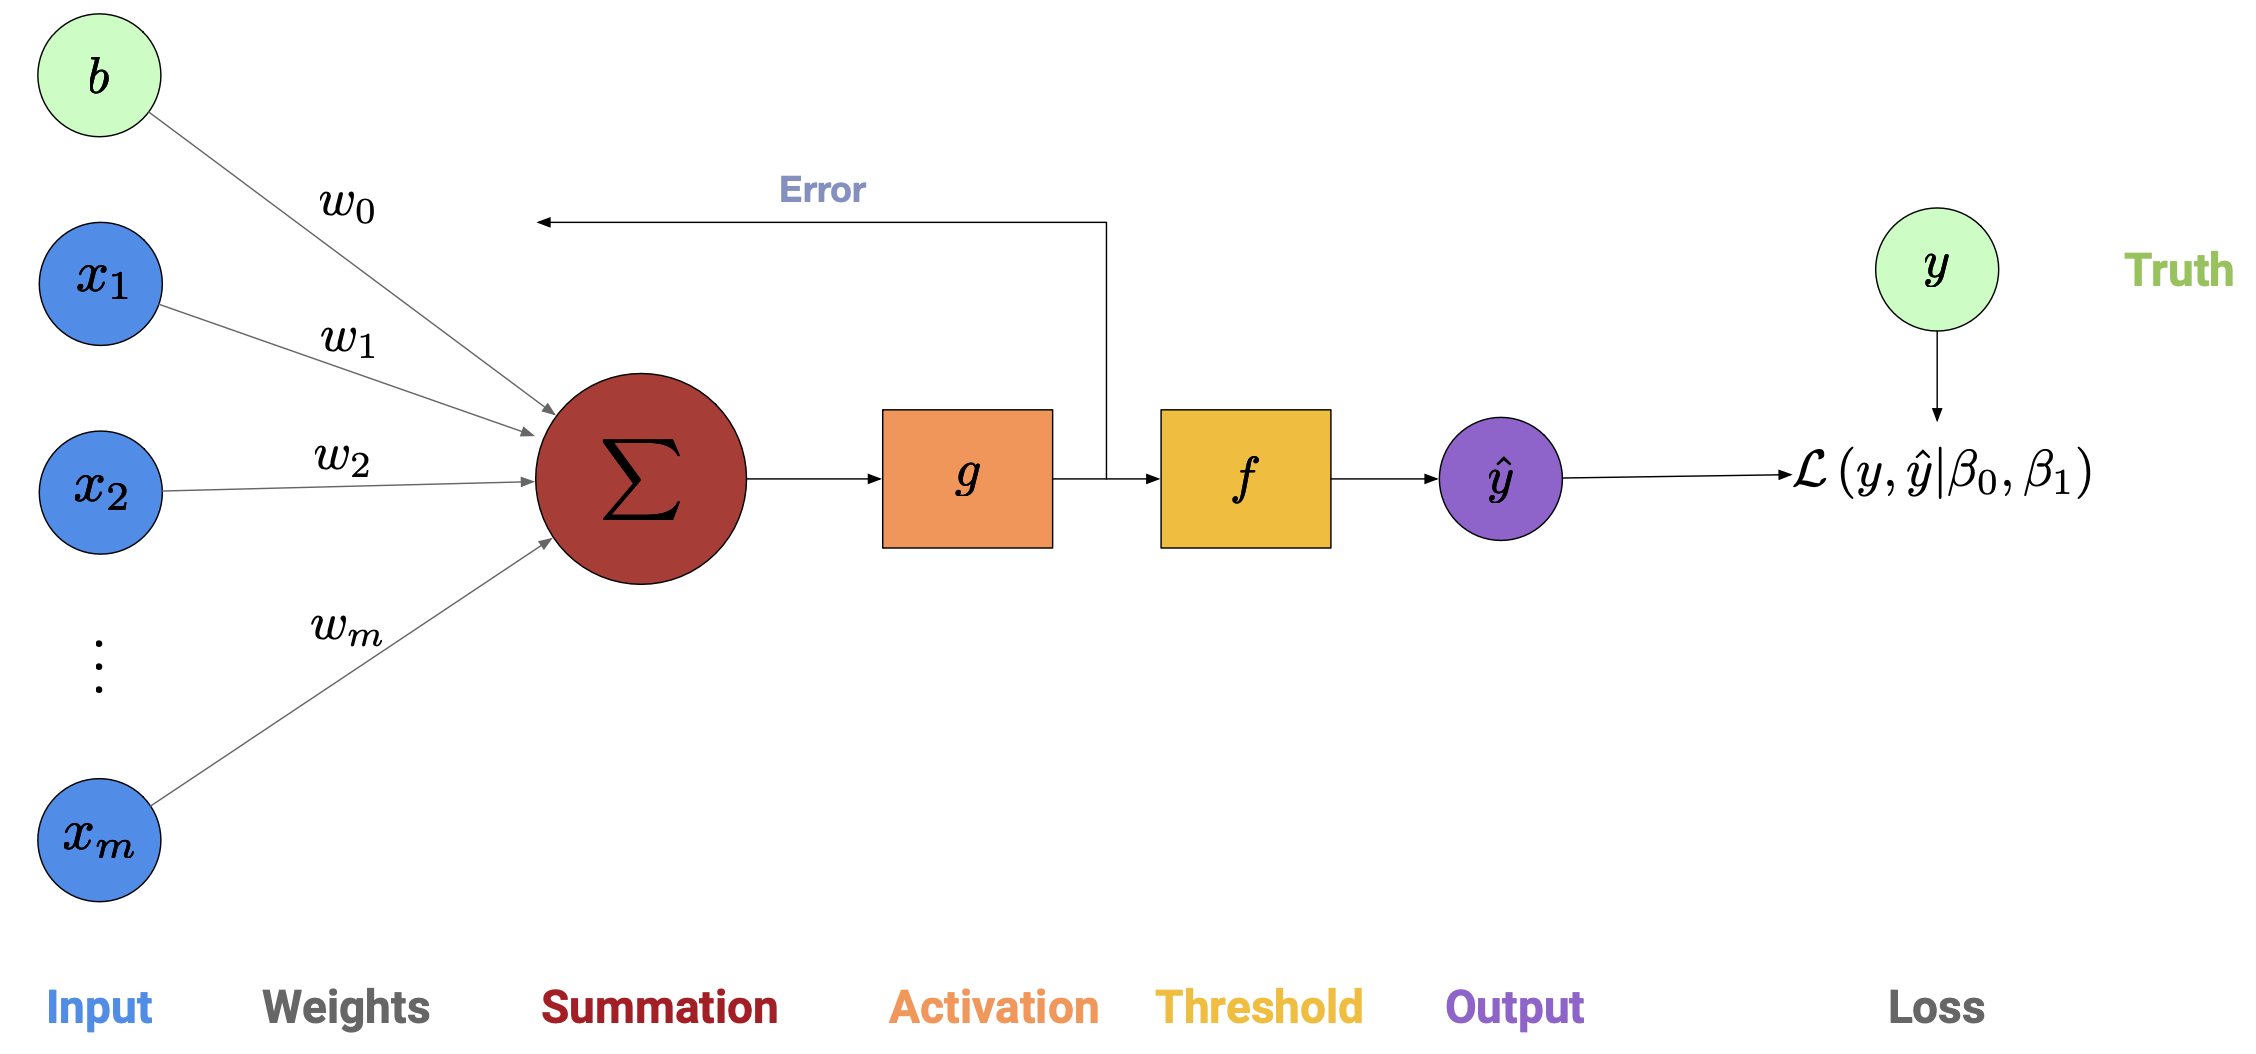
\includegraphics[scale=0.2]{adaline.png}
    \caption{ADALINE}
    \label{}
\end{figure}\end{center}

\subsubsection{Widrow-Hoff Delta Rule}
(Gradient Descent Rule for ADALINE)
\begin{enumerate}[$\bullet$]
    \item \textbf{Original: }$$W=W+\eta(y^{(j)}-z)x^{(j)}$$
    \item \textbf{Unit-norm: }$$W=W+\eta(y^{(j)}-z)\frac{x^{(j)}}{\|x^{(j)}\|}$$
    where $\|x\|=\sqrt{x_1^2+x_2^2+\cdots+x_m^2}$
\end{enumerate}

\textbf{The Perceptron and ADALINE use variants of the delta rule!}
\begin{enumerate}[(1)]
    \item \textbf{Perceptron}: Output used in delta rule is $\hat{y}=g(x^TW)$; $W=W+\eta(y^{(j)}-{\hat{y}}^{(j)})x^{(j)}$
    \item \textbf{ADALINE}: Output used to estimate weights is $z=x^TW$. $W=W+\eta(y^{(j)}-z)x^{(j)}$
\end{enumerate}

\subsection{Logistic Regression (Binary-class Output)}
\subsubsection{Generative and Discriminative Classifiers}
The most important difference between naive Bayes and logistic regression is that \underline{logistic regression} is a \textbf{discriminative classifier} while \underline{naive Bayes} is a \textbf{generative classifier}.

Suppose we want to classify class $A$ (dogs) and class $B$ (cats) (More genearl form: assign a class $c\in C$ to a document $d\in D$):
\begin{enumerate}[(1)]
    \item \underline{\textbf{Generative model:}} A generative model would have the goal of understanding what dogs look like and what cats look like. You might literally ask such a model to ‘generate’, i.e., draw, a dog.\\
    e.g. \textbf{naive Bayes:} we do not directly compute the probability that the document $d$ belongs to each class $c$, $P(c|d)$. We compute likelihood $P(d|c)$ and prior probability $P(c)$ to generate best estimation $\hat{c}$. (i.e., we want to know what should the distribution of a document $d$ in class $c$ be like.) $$\hat{c}=\argmax_{c\in C}P(d|c)P(c)$$
    \item \underline{\textbf{Discriminative model:}} A discriminative model, by contrast, is only trying to learn to distinguish the classes (perhaps without learning much about them). That is we want to directly computing $P(c|d)$.
\end{enumerate}

\subsubsection{Sigmoid function}
The goal of binary logistic regression is to train a classifier that can make a binary decision about the class of a new input observation.

The input observation is $x=[x_1,...,x_m]^T$ and the output $y$ is either $1$ or $0$. Instead of using the optimal weights of each feature $x_i$ and binary activation function (\textbf{threshold}: $\hat{y}=1$ if $z\geq 0$ and $\hat{y}=0$ otherwise) to estimate  in Perceptron and ADALINE, \textbf{we want to estimate the probability $P(y=1|x)$.}

However, \underline{the weighted sum $z=x^TW=\sum_{i=1}^mw_ix_i+b$ ranges $-\infty$ to $\infty$}. We want to \textbf{force the $z$ to be a legal probability}, that is, to lie between $0$ and $1$.

The \textbf{sigmoid function} $\sigma(z)=\frac{1}{1+e^{-z}}$ can be used as acitivation for this purpose, $P(y=1|x)=\sigma(x^TW)$. Since $1-\sigma(x)=\sigma(-x)$, $P(y=0|x)=\sigma(-x^TW)$.

\subsubsection{Cross-entropy Loss Function}
We choose the parameters $W$ that maximize the log probability of the true $y$ labels in the training data given the observations $x$. The conditional probability
\begin{equation}
    \begin{aligned}
        p(y|x)=\left\{\begin{matrix}
            \hat{y},&y=1\\
            1-\hat{y},&y=0
        \end{matrix}\right.=\hat{y}^y(1-\hat{y})^{1-y}
    \end{aligned}
    \nonumber
\end{equation}
To maximize the probability, we log both sides:
\begin{equation}
    \begin{aligned}
        \log p(y|x)=y\log\hat{y}+(1-y)\log(1-\hat{y})
    \end{aligned}
    \nonumber
\end{equation}
Then, we want the $\hat{y}$ to maximize the probability (also the logarithm of the probability):
\begin{equation}
    \begin{aligned}
        \hat{y}^*&=\argmax_{\hat{y}\in[0,1]}\log p(y|x)\\
        &=\argmin_{\hat{y}\in[0,1]}-\log p(y|x)\\
        &=\argmin_{\hat{y}\in[0,1]}-(y\log\hat{y}+(1-y)\log(1-\hat{y}))
    \end{aligned}
    \nonumber
\end{equation}
The right hand side is exactly the \textbf{cross-entropy loss function}:
$$L(y,\hat{y})=-(y\log\hat{y}+(1-y)\log(1-\hat{y}))$$
where $\hat{y}^{(i)}=\sigma(w^Tx^{(i)}+b)$
\begin{equation}
    \begin{aligned}
        \frac{\partial L(y^{(i)},\hat{y}^{(i)})}{\partial w_j}=\left(\sigma(w^Tx^{(i)}+b)-y^{(i)}\right)x_j^{(i)}=(\hat{y}^{(i)}-y^{(i)})x_j^{(i)}
    \end{aligned}
    \nonumber
\end{equation}

The risk (Binary Cross-Entropy Cost) of a weight $W$ is $$J(W)=-\frac{1}{n}\sum_{i=1}^n(y^{(i)}\log\hat{y}^{(i)}+(1-y^{(i)})\log(1-\hat{y}^{(i)}))$$
\begin{equation}
    \begin{aligned}
        \frac{\partial J(w,b)}{\partial w_j}=\frac{1}{n}\sum_{i=1}^n\left(\sigma(w^Tx^{(i)}+b)-y^{(i)}\right)x_j^{(i)}
    \end{aligned}
    \nonumber
\end{equation}

\subsubsection{Algorithm}
\begin{enumerate}[$\bullet$]
    \item Initialize weights (including a bias term) to zero, e.g. $W=[w,b]=0^{m+1}$.
    \item Under each training epoch: Compute for each sample $\left\langle x^{(i)},y^{(i)}\right\rangle\in D$
    \begin{enumerate}[$\cdot$]
        \item A prediction $\hat{y}^{(i)}=g({x^{(i)}}^TW)$
        \item Prediction error $e^{(i)}=y^{(i)}-\hat{y}^{(i)}$
        \item Weighted update $W=W+\eta e^{(i)}x^{(i)}=W-\eta \nabla L(W)$
    \end{enumerate}
\end{enumerate}

\subsection{Softmax Regression (Multi-class Output)}
\subsubsection{Multi-Class Classification and Multi-Label Classification}
\begin{definition}
    \underline{Multi-Class Classification} is a process for assigning each sample exactly one class. In this case, classes are considered mutually exclusive (no intersection).
\end{definition}
\begin{center}\begin{figure}[htbp]
    \centering
    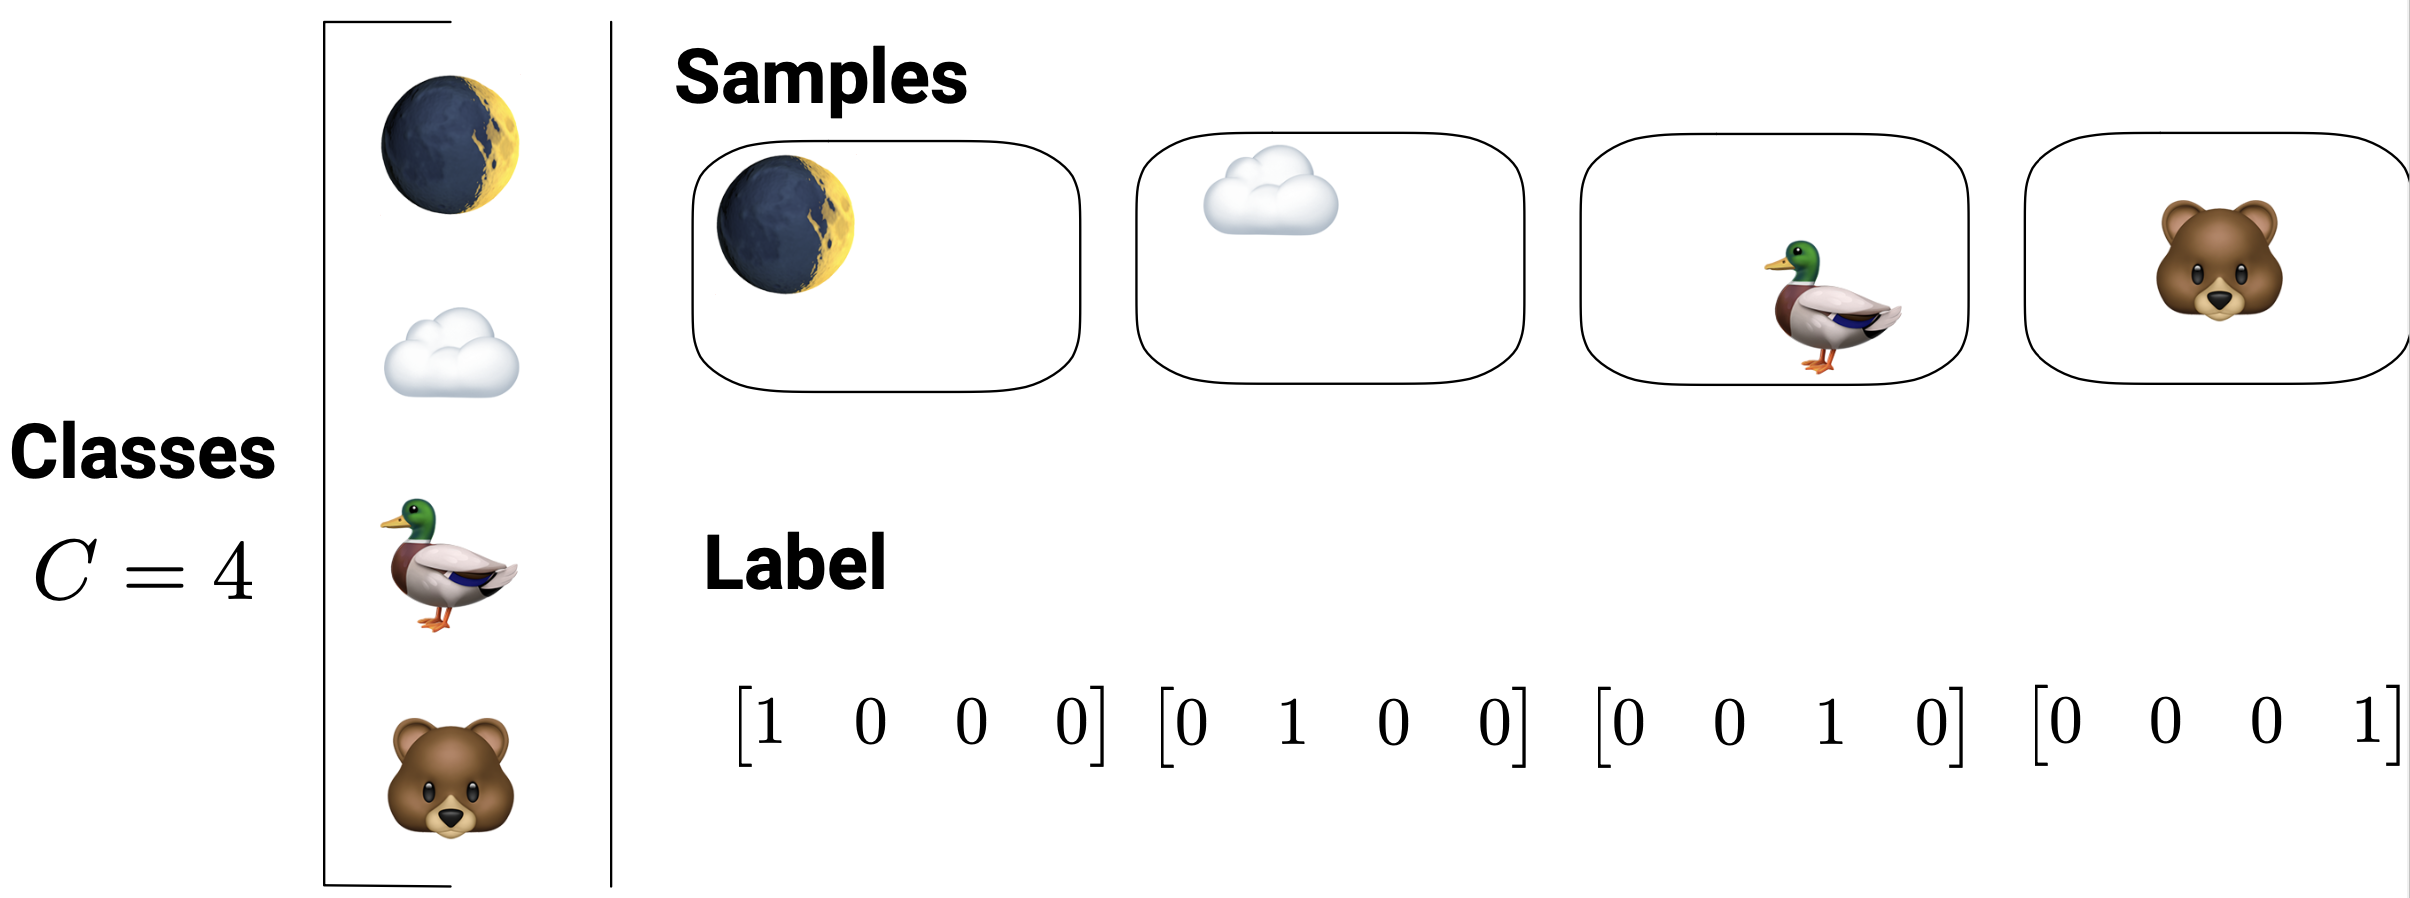
\includegraphics[scale=0.13]{multi-class.png}
    \caption{Multi-Class Classification}
    \label{}
\end{figure}\end{center}
\begin{definition}
    \underline{Multi-Label Classification} or annotation allows for each sample to have 1 or more classes assigned to it. In this case, classes are mutually non-exclusive (one common element).
\end{definition}
\begin{center}\begin{figure}[htbp]
    \centering
    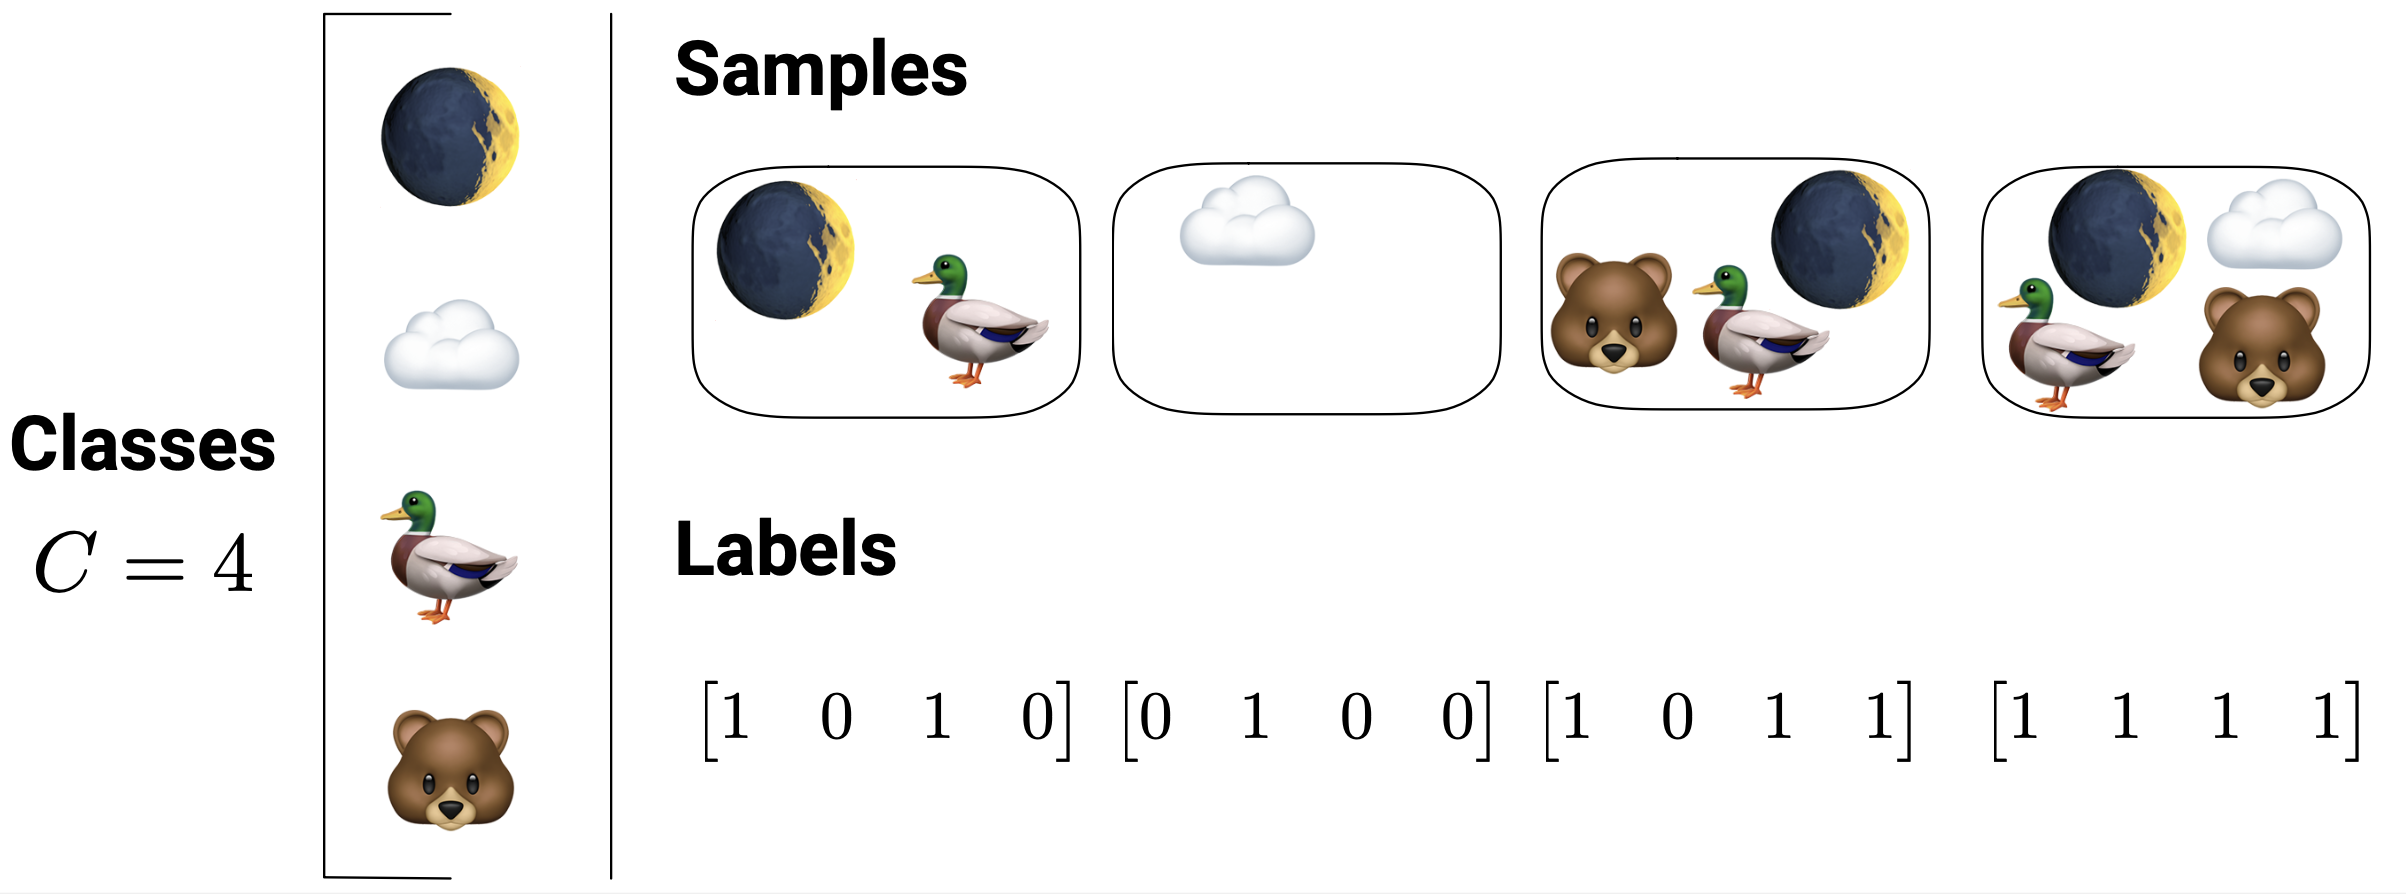
\includegraphics[scale=0.13]{multi-label.png}
    \caption{Multi-Label Classification}
    \label{}
\end{figure}\end{center}

We can show some examples of activation layer and loss choice in different probelms.
\begin{center}\begin{figure}[htbp]
    \centering
    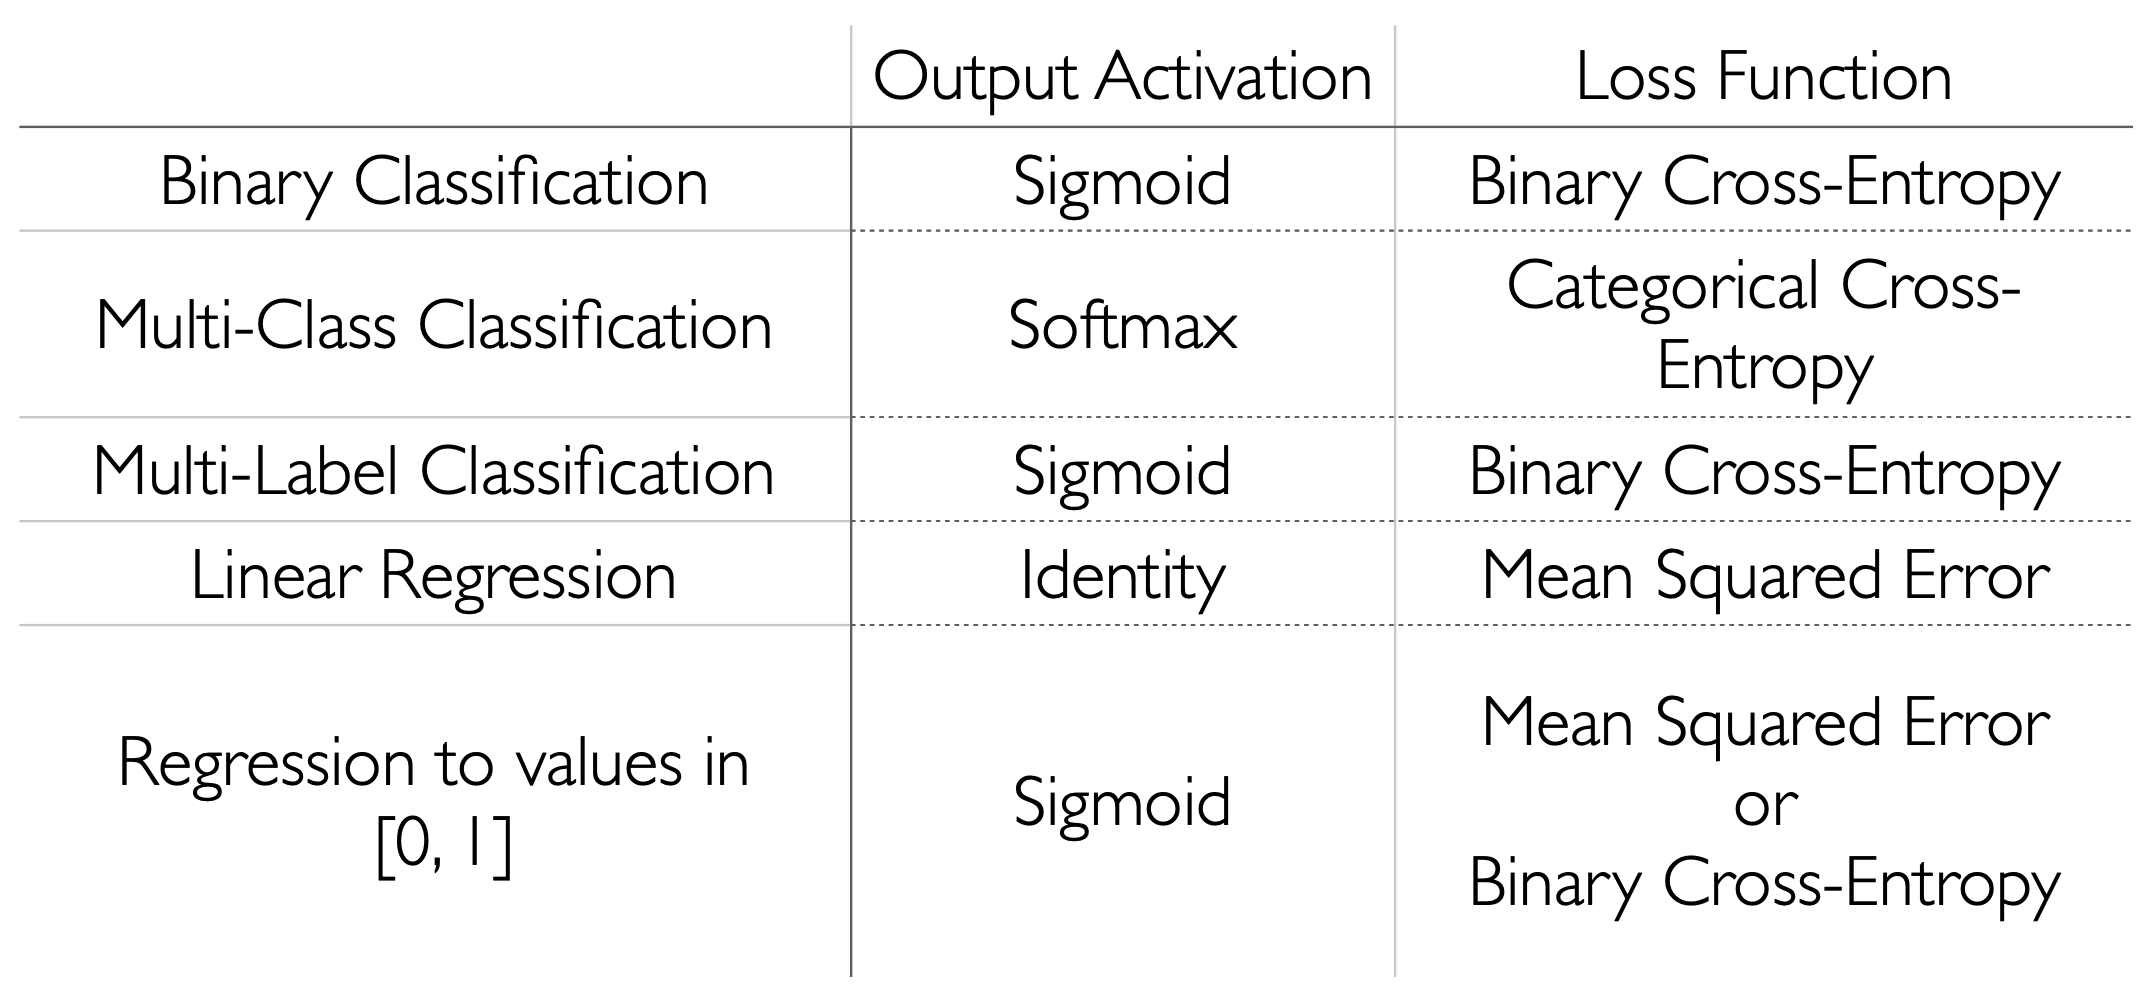
\includegraphics[scale=0.15]{exampleofact.png}
    \caption{Examples of Activation Layer and Loss Choice}
    \label{}
\end{figure}\end{center}

\subsubsection{One-hot Encoding}
\begin{definition}
    \underline{One-hot encoding} is the process of assigning a single location within a vector to represent a given category.
\end{definition}
\begin{center}\begin{figure}[htbp]
    \centering
    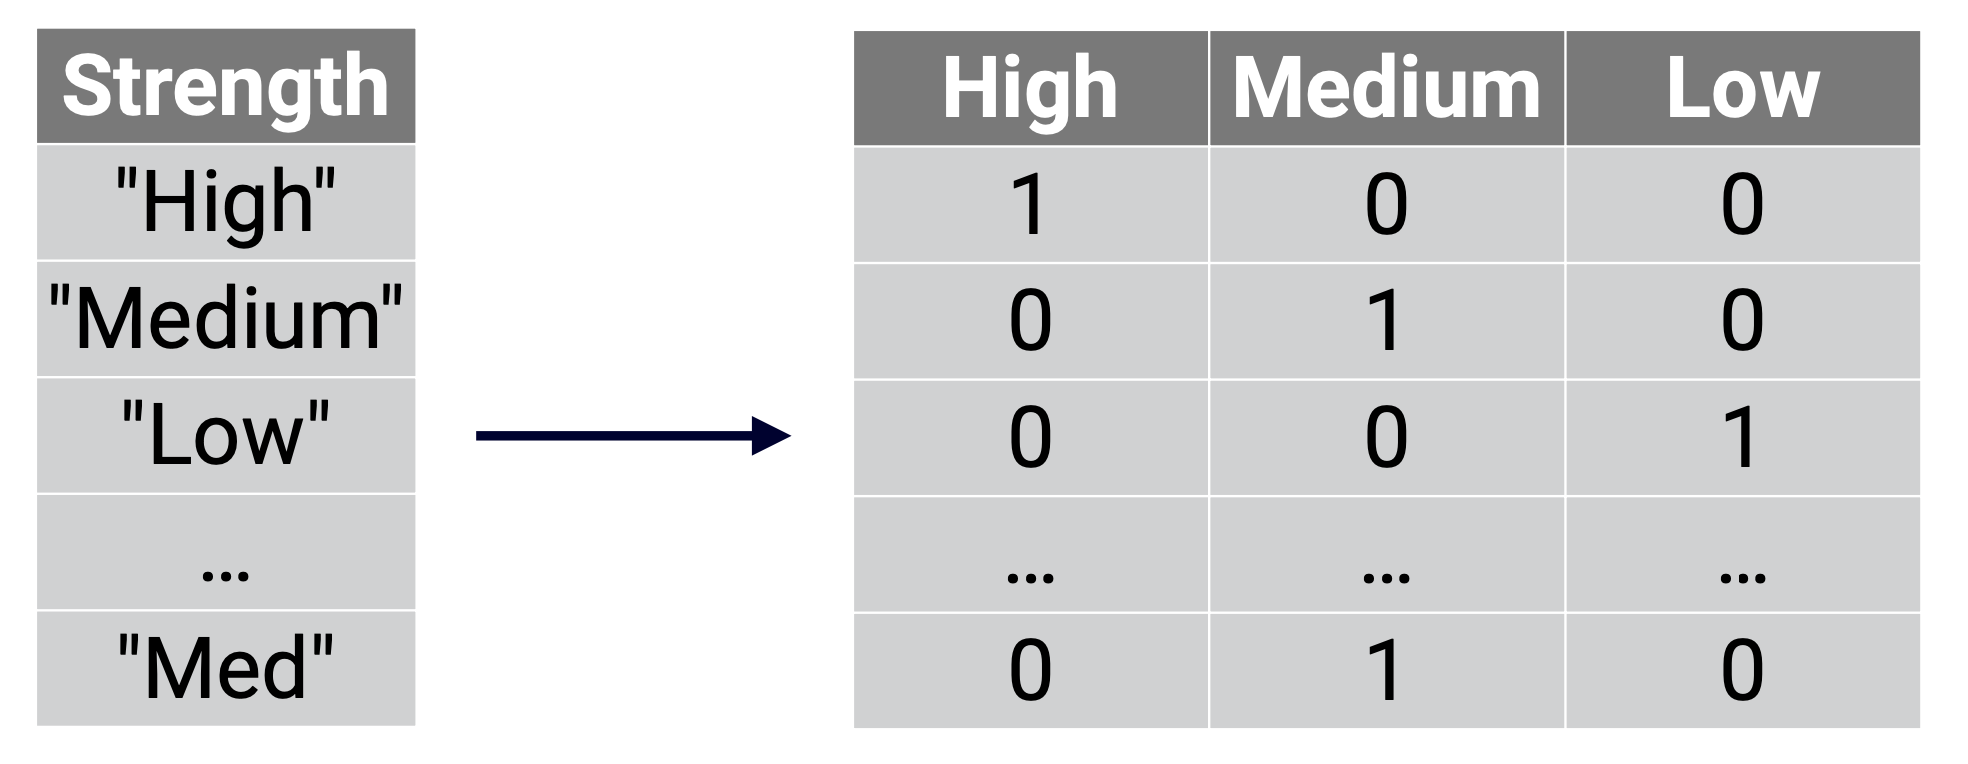
\includegraphics[scale=0.15]{ohe.png}
    \caption{One-hot encoding}
    \label{}
\end{figure}\end{center}
\textbf{Examples:}
\begin{enumerate}
    \item $\mathbf{z}=[4]_{1 \times 1} \rightarrow\left[\begin{array}{lllll}
        0 & 0 & 0 & 0 & 1
        \end{array}\right]_{1 \times 5}$
    \item $\mathbf{y}=\left[\begin{array}{lll}
        3 & 0 & 2
        \end{array}\right]_{1 \times 3} \rightarrow\left[\begin{array}{llll}
        0 & 0 & 0 & 1 \\
        1 & 0 & 0 & 0 \\
        0 & 0 & 1 & 0
        \end{array}\right]_{3 \times 4}$
    \item $\mathbf{v}=\left[\begin{array}{lllll}
        5 & 0 & 4 & 4 & 3
        \end{array}\right]_{1 \times 5} \rightarrow\left[\begin{array}{llllll}
        0 & 0 & 0 & 0 & 0 & 1 \\
        1 & 0 & 0 & 0 & 0 & 0 \\
        0 & 0 & 0 & 0 & 1 & 0 \\
        0 & 0 & 0 & 0 & 1 & 0 \\
        0 & 0 & 0 & 1 & 0 & 0
        \end{array}\right]_{5 \times 6}$
\end{enumerate}
\textbf{Usefulness of Encodings}
\begin{enumerate}
    \item Close to a traditional design matrix for linear regression that uses a codified dummy variable structure. e.g. FALSE (0) or TRUE (1)
    \item Reduce the size of data stored by using numbers instead of
    strings.
    \item Poor if there are too many unique values (e.g. text messages on a phone.)
\end{enumerate}




\subsubsection{Softmax function}
\begin{definition}
    \underline{Softmax function} or \underline{normalized exponential function} converts between real valued numbers to values between 0 and 1
\end{definition}
\textbf{Softmax:} $S_j(\vec{x})=\frac{e^{x_j}}{\sum_{i=1}^ne^{x_i}}$, $$S(\vec{x})=\left[\frac{e^{x_1}}{\sum_{i=1}^ne^{x_i}},\frac{e^{x_2}}{\sum_{i=1}^ne^{x_i}},\cdots, \frac{e^{x_n}}{\sum_{i=1}^ne^{x_i}}\right]^T$$
We can show the softmax function has the following properties:
\begin{enumerate}[(1)]
    \item First-derivative: $$\frac{\partial S_j(\vec{x})}{\partial x_j}=S_j(\vec{x})[1-S_j(\vec{x})]$$
    \item Stabilizing softmax: $$S_j(\vec{x}+c)=\frac{e^{x_j+c}}{\sum_{i=1}^ne^{x_i+c}}=\frac{e^{x_j}}{\sum_{i=1}^ne^{x_i}}=S_j(\vec{x})$$
    We can minus $\max_{i} x_i$ to avoid overflow in softmax function. (numerical issue) i.e., $S_j(\vec{x}-(\max_{i} x_i))=S_j(\vec{x})$
\end{enumerate}

\subsubsection{Categorical Cross-entropy Loss Function}
\begin{definition}
    \underline{Categorical Cross-entropy Loss} is a way to quantify the difference between a "true" values $\{y_c\}_{c\in C}$ and an estimated $\{\hat{y}_c\}_{c\in C}$ across $C$ categories.
\end{definition}
Note: $y$ needs one-hot encoding firstly, $\hat{y}$ are estimated probability.
$$L(y,\hat{y})=-\sum_{c\in C}\left(y_c\cdot \log(\hat{y}_c)\right)$$

\begin{definition}
    \underline{Categorical Cross-entropy Cost} is a way of quantifying the cost over multiple points from different categories.
\end{definition}
$$J(W)=\frac{1}{n}\sum_{i=1}^n L(y_i,\hat{y}_i)=-\frac{1}{n}\sum_{i=1}^n\sum_{c\in C}\left(y_{i,c}\cdot \log(\hat{y}_{i,c})\right)$$














\subsection{Deep Feedforward Networks}

\subsubsection{Definition}
In any neural network, a \underline{dense layer} is a layer that is deeply connected with its preceding layer which means the neurons of the layer are connected to \textit{every neuron} of its preceding layer.

\begin{definition}
    \underline{Deep feedforward networks}, \underline{feedforward neural networks}, \underline{multilayer perceptrons (MLPs)}, or \underline{dense neural networks} form the foundations of deep learning models. Learning occurs in only one direction: \textbf{forward}. There are \textbf{no feedback} connections in whichoutputs of the model are fed back into itself. There are no cycles or loops present. Information must flow from the input layer, through one or more hidden layers, before reaching the output.
\end{definition}

\begin{center}\begin{figure}[htbp]
    \centering
    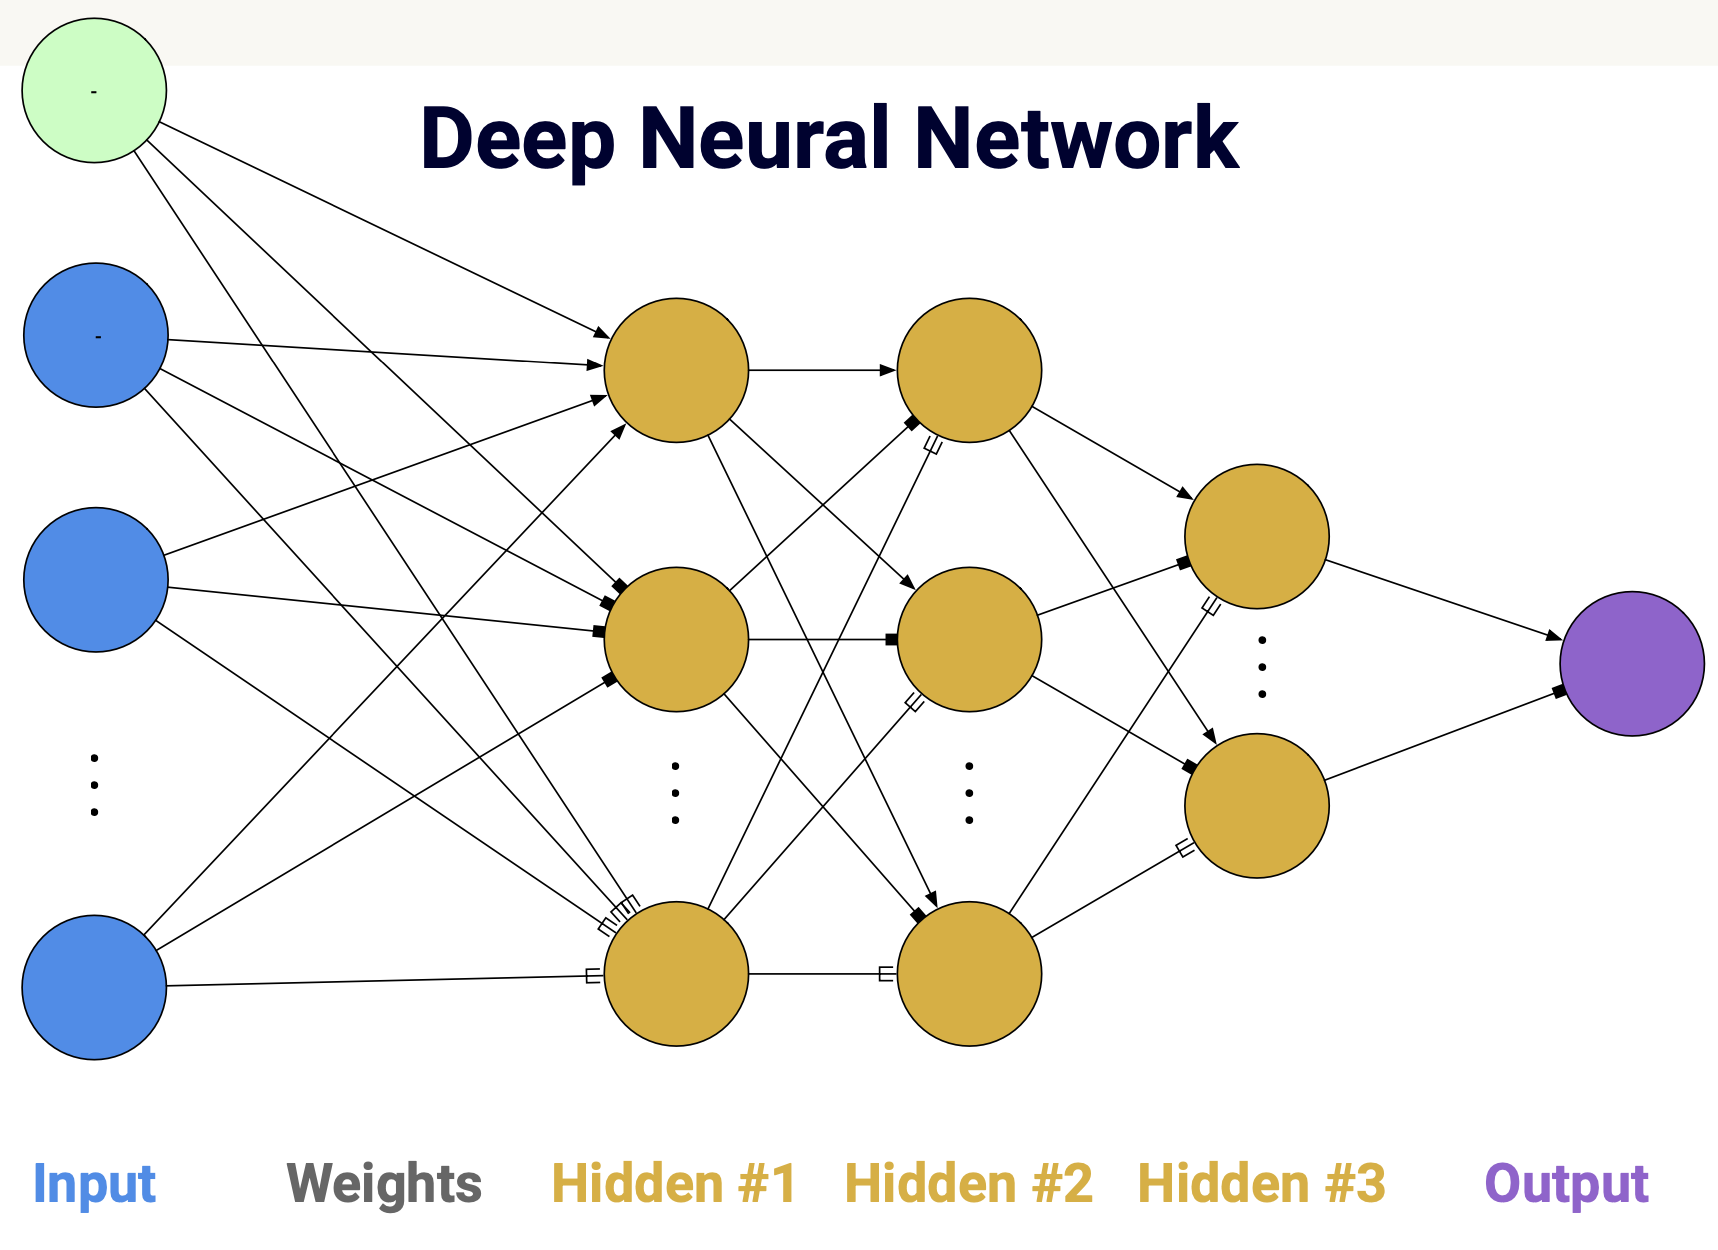
\includegraphics[scale=0.13]{deep.png}
    \caption{Deep Neural Network}
    \label{}
\end{figure}\end{center}
A deep neural network contains \textit{Input Layer}, \textit{Hidden Layer}, and \textit{Output Layer}.


\subsubsection{Universal Approximation Theorem}
Universal Approximation Theorem, in its lose form, states that a \textbf{feed-forward network} with a \textbf{single hidden layer} containing a finite number of neurons \textbf{can approximate any continuous function}. (Which is also equivalent to having a nonpolynomial activation function)
\begin{theorem}[Universal approximation theorem]
    Fix a continuous function $\sigma: \mathbb{R} \rightarrow \mathbb{R}$ (activation function) and positive integers $d, D\in \mathbb{Z}^+$. The function $\sigma$ is \underline{not a polynomial} $\Leftrightarrow$ for every continuous function $f: \mathbb{R}^d \rightarrow \mathbb{R}^D$ (target function), every compact subset $K$ of $\mathbb{R}^d$, and every $\epsilon>0$ there exists a continuous function $f_\epsilon: \mathbb{R}^d \rightarrow \mathbb{R}^D$ (the layer output) with representation $$f_\epsilon=W_2 \circ \sigma \circ W_1$$
    where $W_2, W_1$ are composable affine maps and o denotes component-wise composition, such that the approximation bound $$\sup _{x \in K}\left\|f(x)-f_\epsilon(x)\right\|<\varepsilon$$
    holds for any $\epsilon$ arbitrarily small (distance from $f$ to $f_\epsilon$ can be infinitely small).
\end{theorem}

\begin{center}\begin{figure}[htbp]
    \centering
    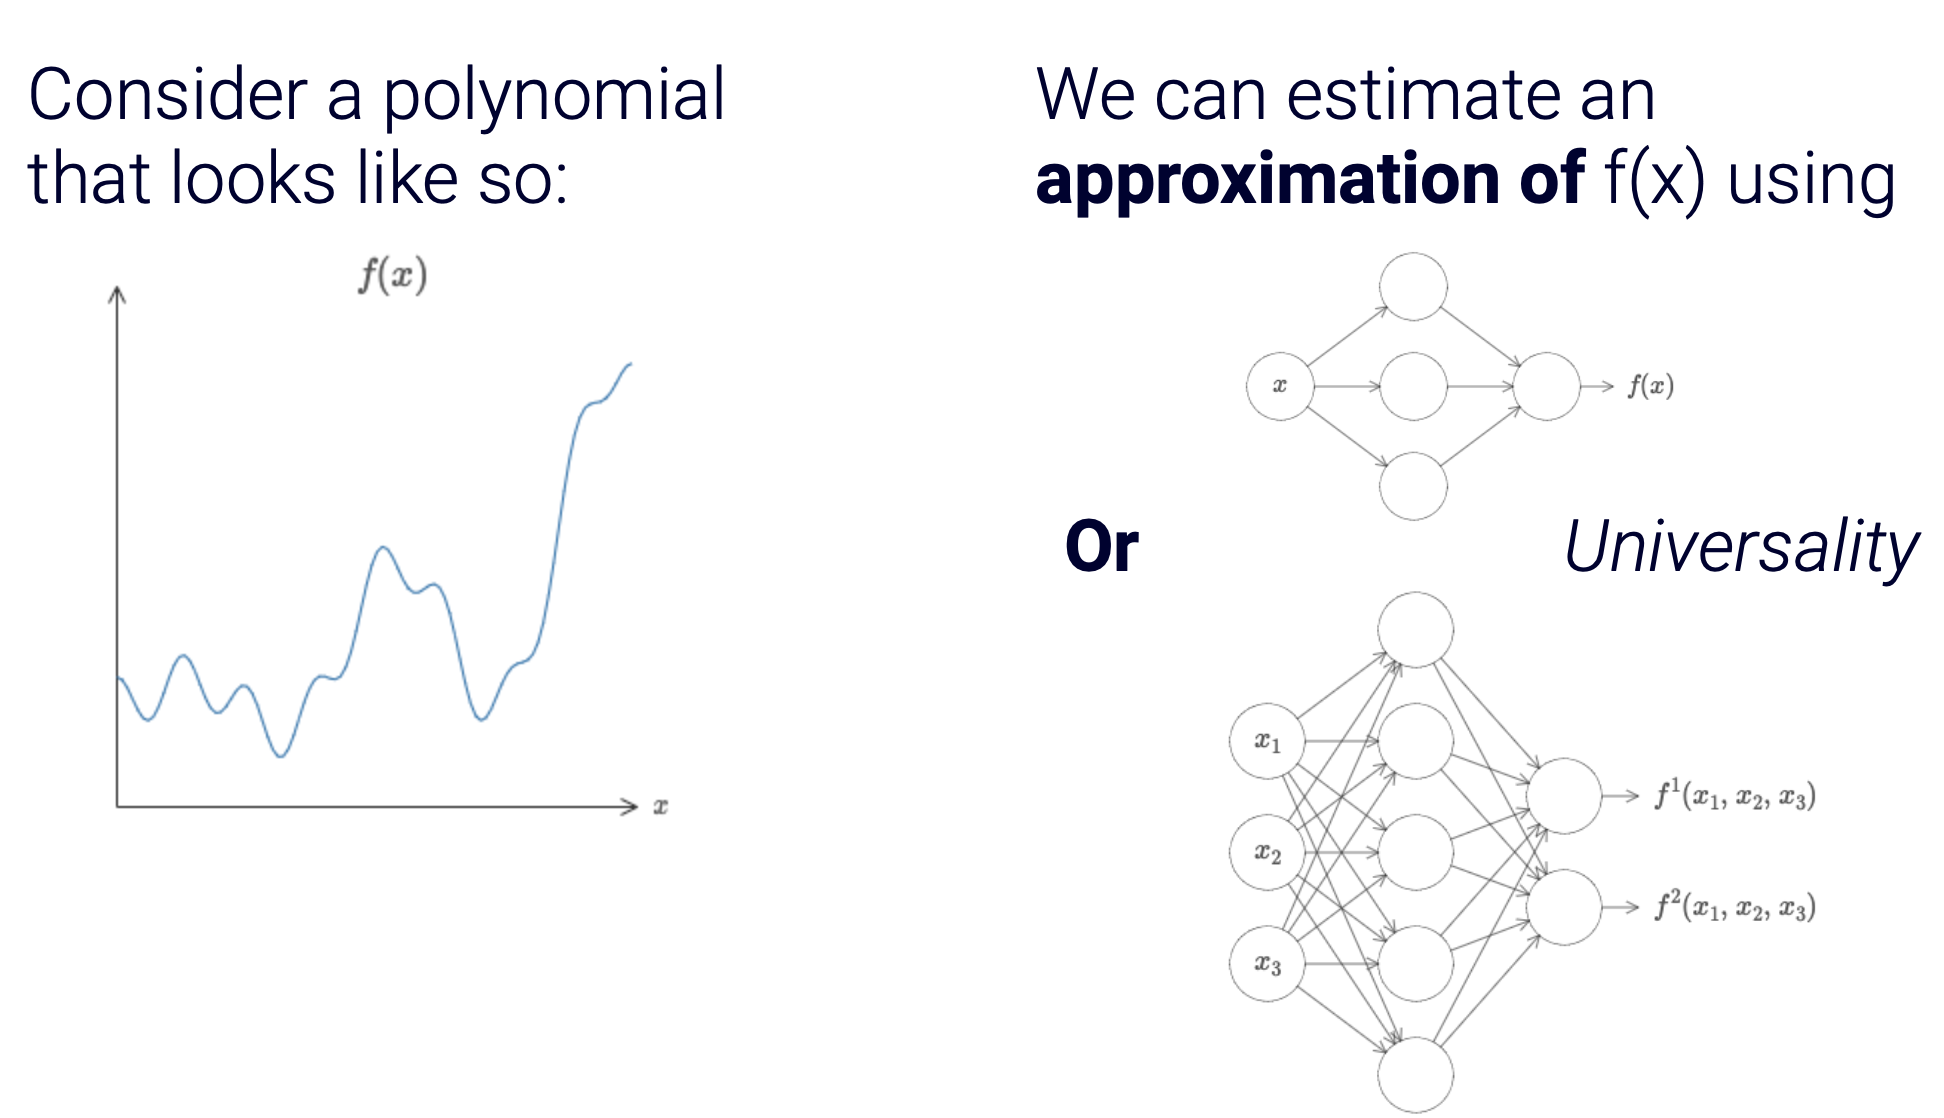
\includegraphics[scale=0.2]{UAT.png}
    \caption{Universal Approximation Theorem}
    \label{}
\end{figure}\end{center}

\subsection{ Mini-batch Optimization}
\subsubsection{Stochastic Gradient Descent (SGD) and Batch Gradient Descent (BGD)}
\textbf{Stochastic Gradient Descent (SGD)}
\begin{enumerate}
    \item Start with a random guess.
    \item For $n$ epochs:
    \begin{enumerate}[1)]
        \item Reorder data
        \item Retrieve an observation $i=1,2,...$ one by one in reordered data:
        \begin{enumerate}[(1)]
            \item Compute gradient on single data point $i$: $\frac{\partial J_i(W)}{\partial W}$
            \item Update parameters:
            $W=W-\alpha \frac{\partial J_i(W)}{\partial W}$
        \end{enumerate}
    \end{enumerate}
    \item Output parameters
\end{enumerate}
\textbf{Note:} "On-line"/"Stochastic" \textbf{Single} Observation Updates

\textbf{Batch Gradient Descent (BGD)}
\begin{enumerate}
    \item Start with a random guess.
    \item For $n$ epochs:
    \begin{enumerate}[1)]
        \item Compute gradients on
        \textbf{all the data}: $\frac{\partial J(W)}{\partial W}$
        \item Update parameters:
        $W=W-\alpha \frac{\partial J(W)}{\partial W}$
    \end{enumerate}
    \item Output parameters
\end{enumerate}
\textbf{Note:} \textbf{All} data used in update
\begin{center}\begin{figure}[htbp]
    \centering
    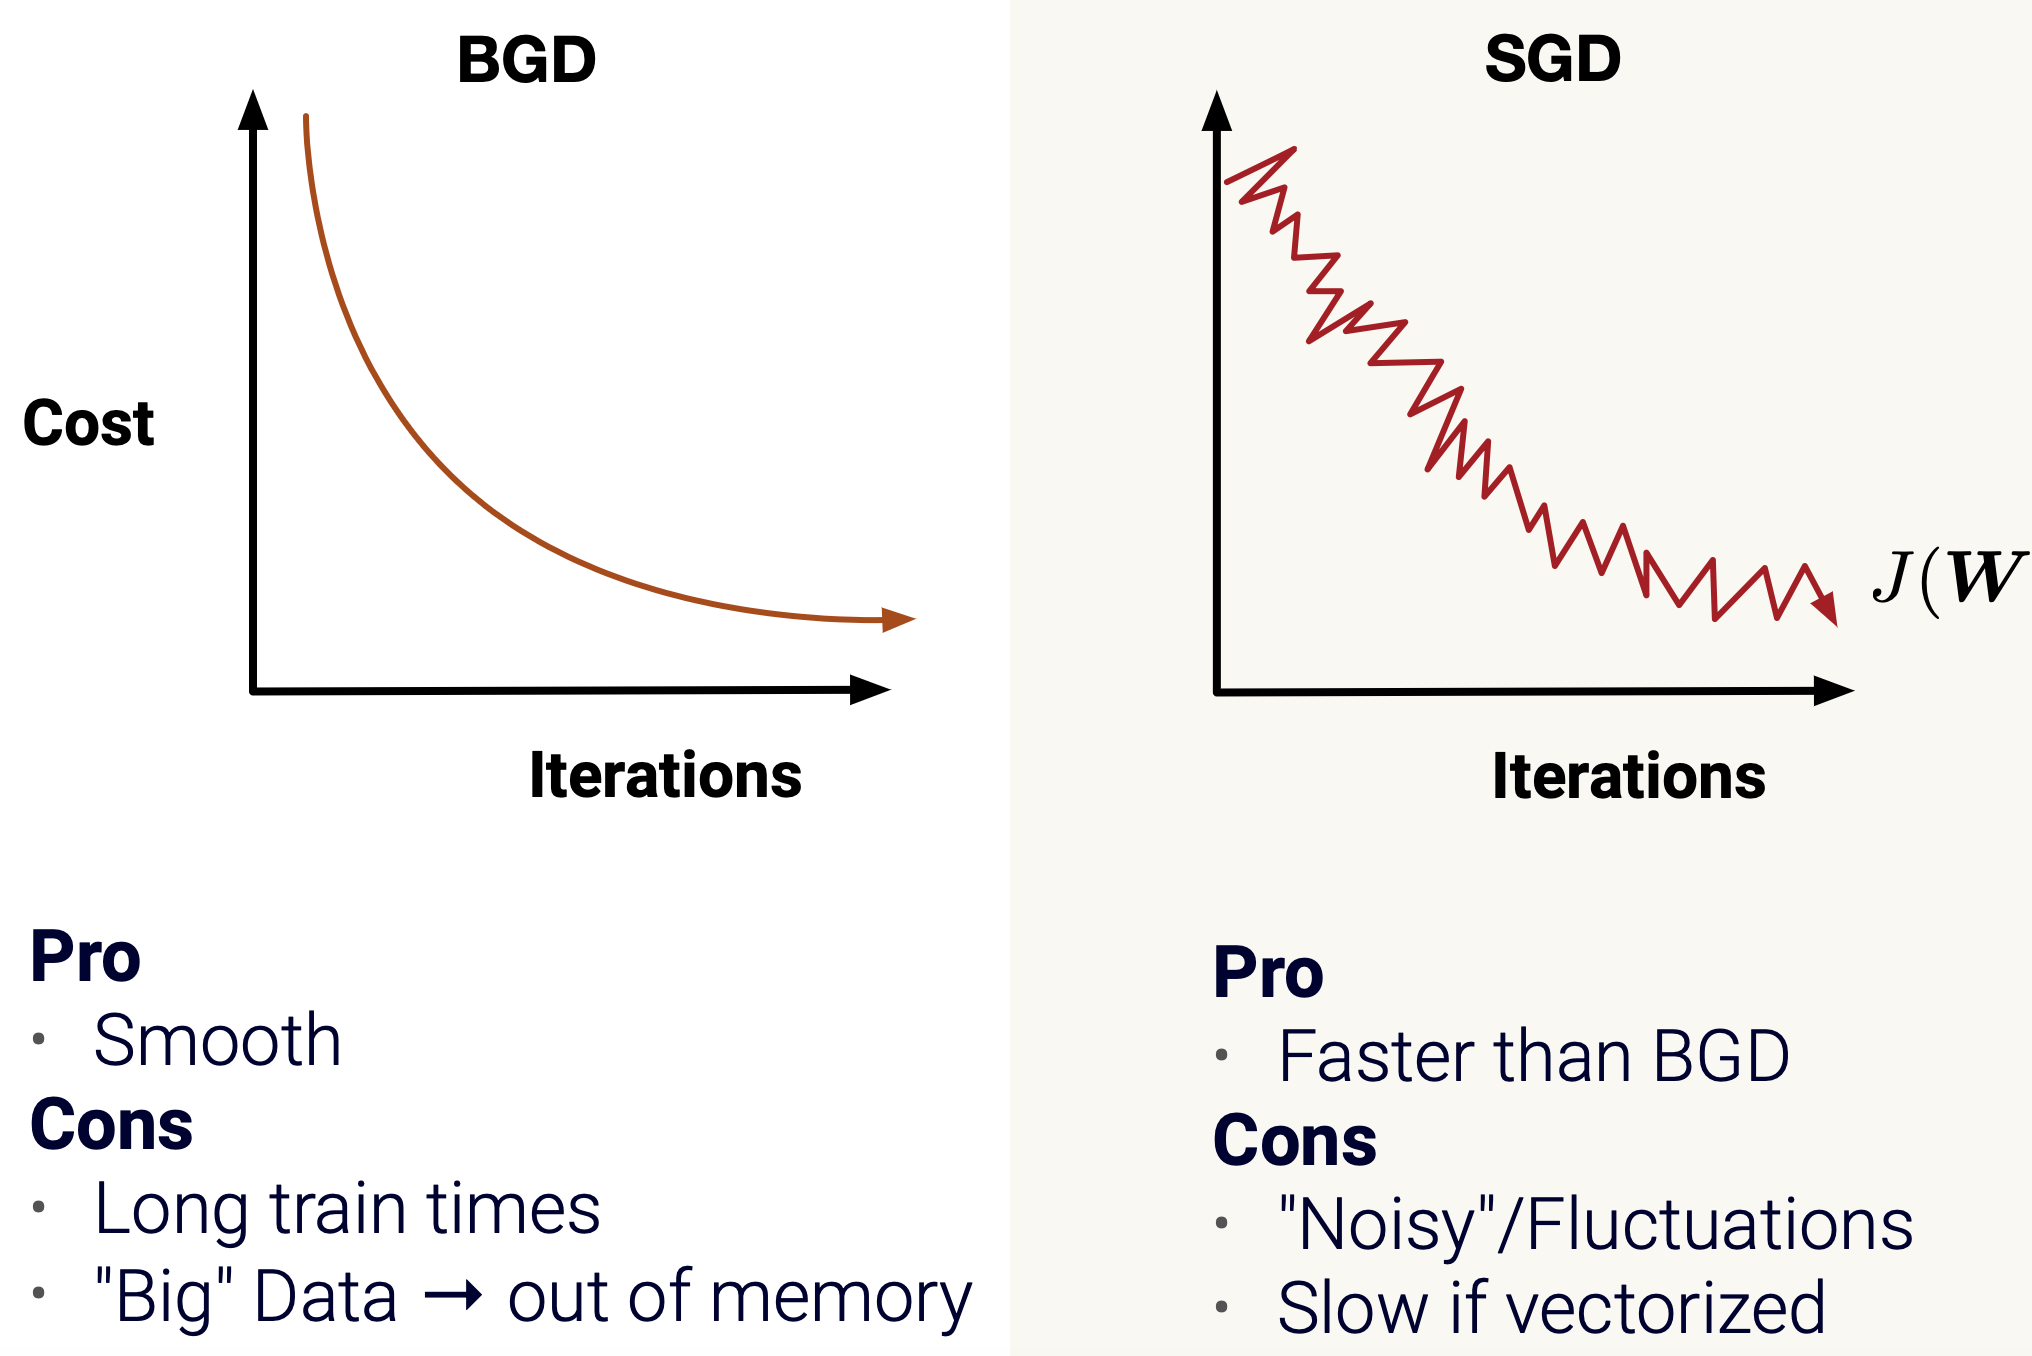
\includegraphics[scale=0.1]{BGDandSGD.png}
    \caption{BGD and SGD}
    \label{}
\end{figure}\end{center}

\subsubsection{Mini-Batch Gradient Descent (MBGD)}
We want a middle ground between SGD and BGD.

\textbf{Mini-Batch Gradient Descent (MBGD)}
\begin{enumerate}
    \item Start with a random guess.
    \item For $n$ epochs:
    \begin{enumerate}[1)]
        \item Reorder data and retrieve a subet of reordered data with size $b$ (batch size)
        \item Retrieve an observation $i=1,2,...b$ one by one in the subet:
        \begin{enumerate}[(1)]
            \item Compute gradient on single data point $i$: $\frac{\partial J_i(W)}{\partial W}$
            \item Update parameters:
            $W=W-\alpha \frac{\partial J_i(W)}{\partial W}$
        \end{enumerate}
    \end{enumerate}
    \item Output parameters
\end{enumerate}
\begin{center}\begin{figure}[htbp]
    \centering
    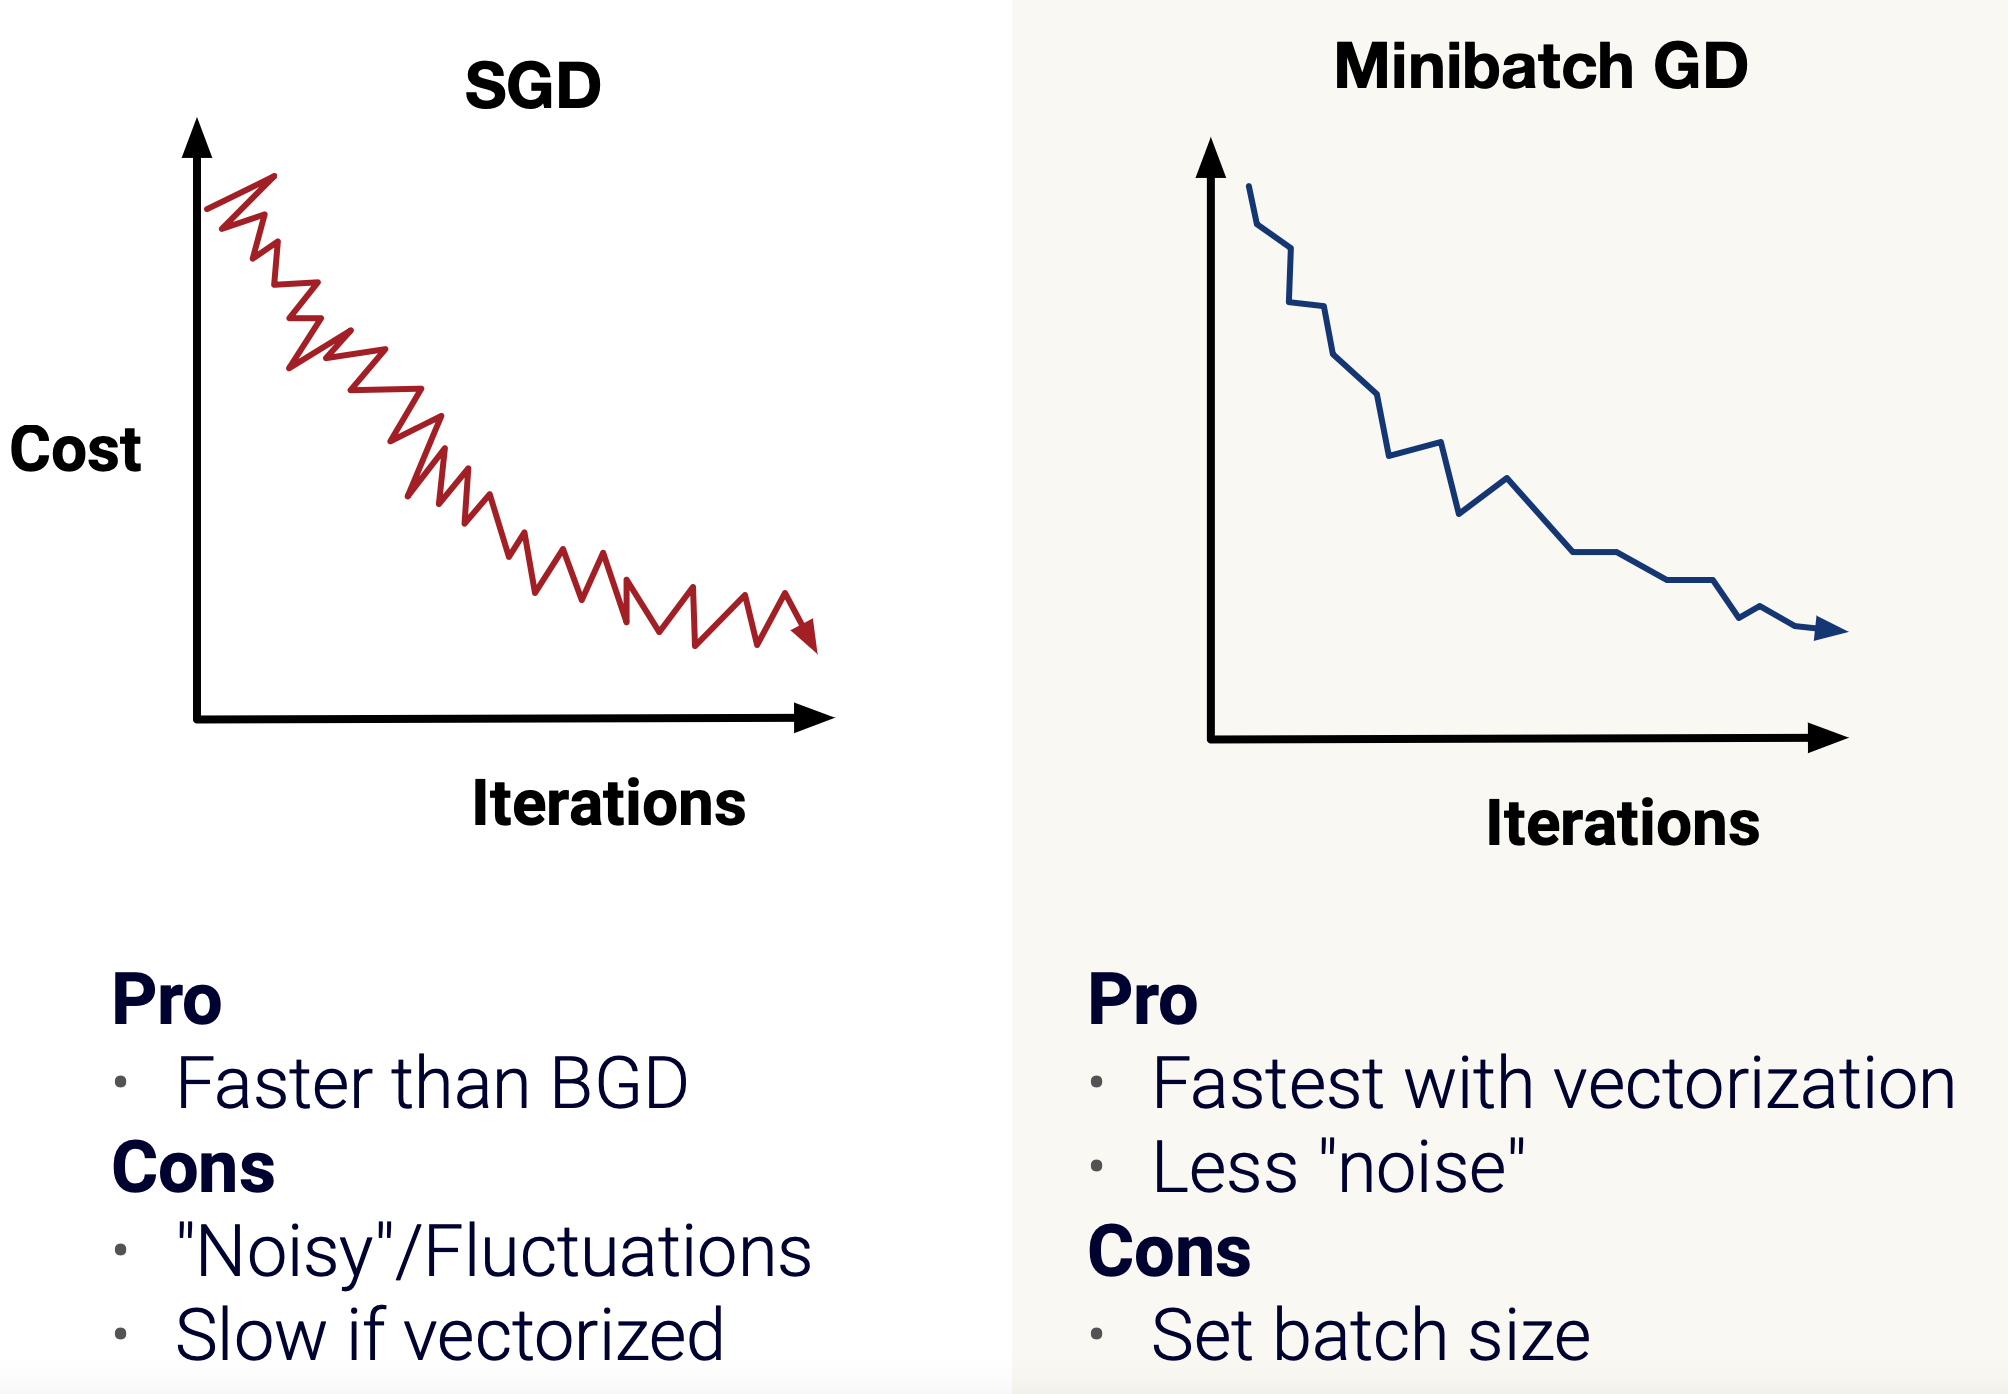
\includegraphics[scale=0.1]{SGDandMBGD.png}
    \caption{SGD and MBGD}
    \label{}
\end{figure}\end{center}

\begin{center}\begin{figure}[htbp]
    \centering
    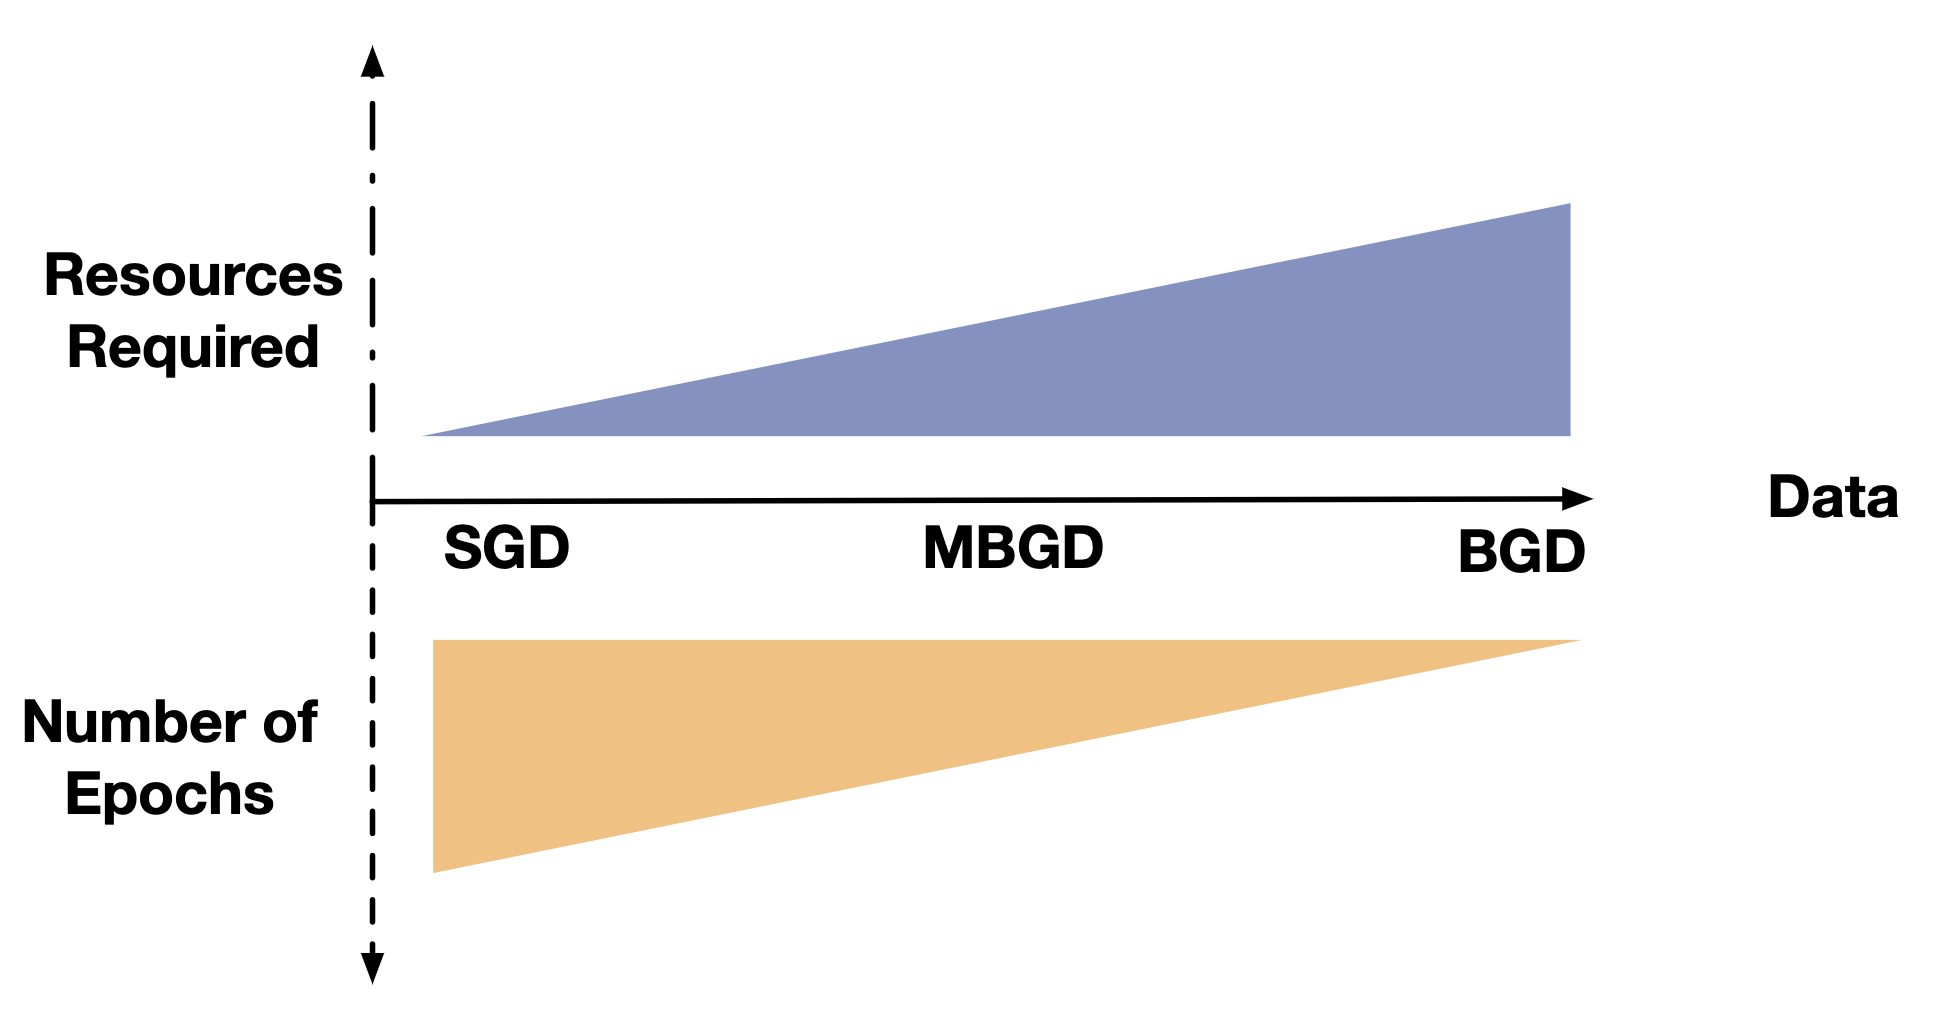
\includegraphics[scale=0.1]{resource.png}
    \caption{Comparison of Approaches}
    \label{}
\end{figure}\end{center}

\subsection{Weight Initialization}
\subsubsection{Xavier Initialization}
Normal distribution with a scale variance by weights. Used on layers where either $TanH$ or $Sigmoid$ is present.
\begin{center}
    Initialize weights for layer $l$ with: $W^{[l]}=W^{[l]}\sqrt{\frac{1}{n^{[l-1]}}}$
\end{center}
where $n^{[l-1]}$ is the number of weights in the last layer. Each weight is sampled by $W_{j,i}^{[l]}\sim \mathcal{N}(0,1)$

\subsubsection{He Activation}
Weight initialization for $ReLU$-powered network.
\begin{center}
    Initialize weights for layer $l$ with: $W^{[l]}=W^{[l]}\sqrt{\frac{2}{n^{[l-1]}}}$
\end{center}
where $n^{[l-1]}$ is the number of weights in the last layer. Each weight is sampled by $W_{j,i}^{[l]}\sim \mathcal{N}(0,1)$

\section{Image Processing}
\subsection{Convolutional Neural Network (CNN)}
\subsubsection{Convolution and Cross-correlation}
Cross-correlation and convolution are both operations applied to images. Cross-correlation means sliding a kernel (filter) across an image. Convolution means sliding a flipped kernel across an image. \textbf{Most convolutional neural networks in machine learning libraries are actually implemented using cross-correlation}, but it doesn't change the results in practice because if convolution were used instead, the same weight values would be learned in a flipped orientation.

We have some \textit{source pixels}, we use a \textit{convolution kernel} (filter) to process the \textit{source pixels}. The output is \textit{destination pixels}.

Given the \textit{source pixels} $\{\textbf{Image}(x,y):x\in [-d_X,d_X],y\in [-d_Y,d_Y]\}$ and \textit{convolution kernel} (filter) $\{K(i,j):i,j\in[-d,d]\}$. $n_X=2d_X+1,n_Y=2d_Y+1$ are image dimension, $f=2d+1$ is the filter dimension. We can generate destination pixels in $(n_X-f+1)\times (n_Y-f+1) = (n_X-2d)\times (n_Y-2d)$

For $x\in [d+1,n_X-d],y\in [d+1,n_Y-d]$
\begin{enumerate}
    \item \textbf{Convolution:}
    \begin{equation}
        \begin{aligned}
            \textbf{CONV}(x,y)=\sum_{i=-d}^d\sum_{j=-d}^d \textbf{Image}(x-i,y-j)K(i,j)
        \end{aligned}
        \nonumber
    \end{equation}
    \item \textbf{Cross-Correlation:}
    \begin{equation}
        \begin{aligned}
            \textbf{CrossCorrelation}(x,y)=\sum_{i=-d}^d\sum_{j=-d}^d \textbf{Image}(x+i,y+j)K(i,j)
        \end{aligned}
        \nonumber
    \end{equation}
\end{enumerate}

\begin{center}\begin{figure}[htbp]
    \centering
    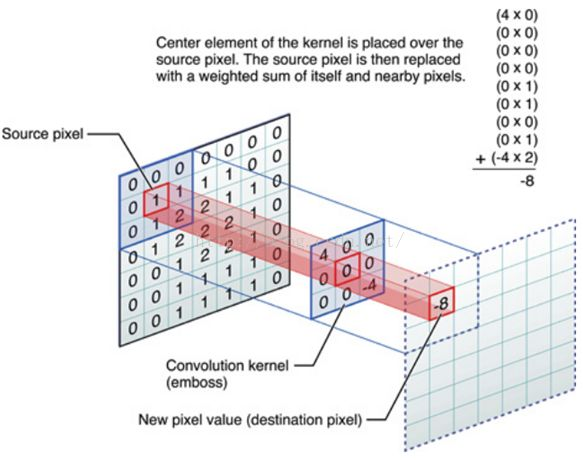
\includegraphics[scale=0.5]{convolution.jpeg}
    \caption{Convolution Used in CNN (actually cross-correlation)}
    \label{}
\end{figure}\end{center}

\subsubsection{Padding (cover the border)}
\begin{definition}
    \underline{Padding} refers to the extension of the input image by adding a border of pixels the image.
\end{definition}

\begin{center}\begin{figure}[htbp]
    \centering
    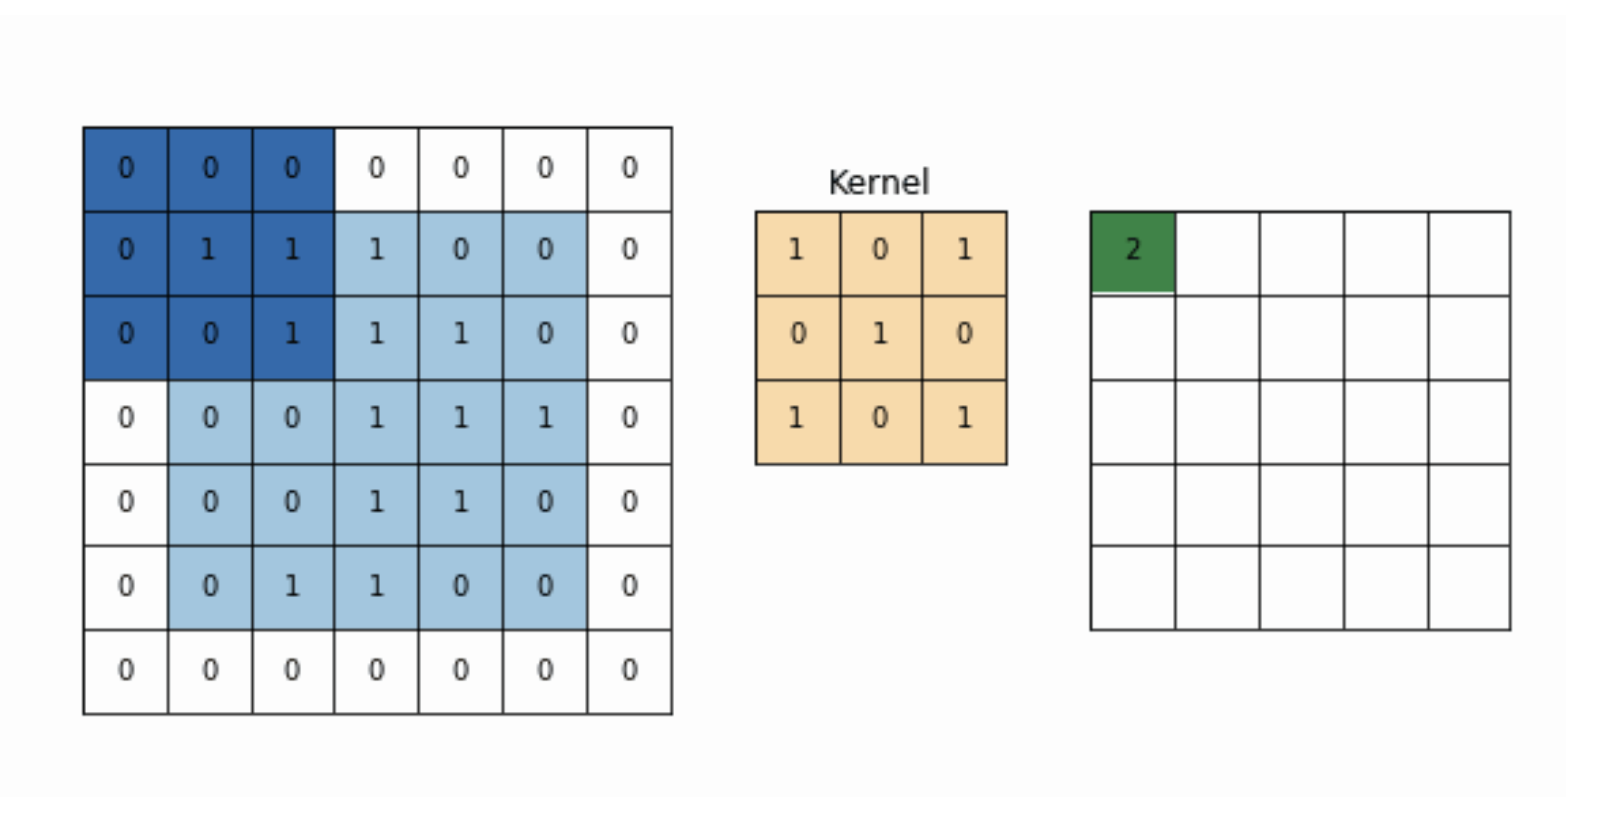
\includegraphics[scale=0.15]{Padding.png}
    \caption{Padding}
    \label{}
\end{figure}\end{center}
Filter with padding outputs the same dimension as \textit{source pixels}.

\subsubsection{Stride}
\begin{definition}
    \underline{Stride} refers to the sliding distance of the filter/kernel over spatial locations.
\end{definition}
The default stride or strides in two dimensions is (1,1) for the height and the width movement.

For example, the stride can be changed to (2,2). This has the effect of moving the filter two pixels right for each horizontal movement of the filter and two pixels down for each vertical movement of the filter when creating the feature map.

The new dimension of the output would be
\begin{equation}
    \begin{aligned}
        \left\lfloor \frac{n_X-1}{s}+1\right\rfloor\times\left\lfloor \frac{n_Y-1}{s}+1\right\rfloor
    \end{aligned}
    \nonumber
\end{equation}

\subsection{Other Layer Types}
\subsubsection{Pooling}
\begin{definition}
    \underline{Pooling} refers to the process of downsampling features by aggregating values at places in the feature map.
\end{definition}
\begin{center}\begin{figure}[htbp]
    \centering
    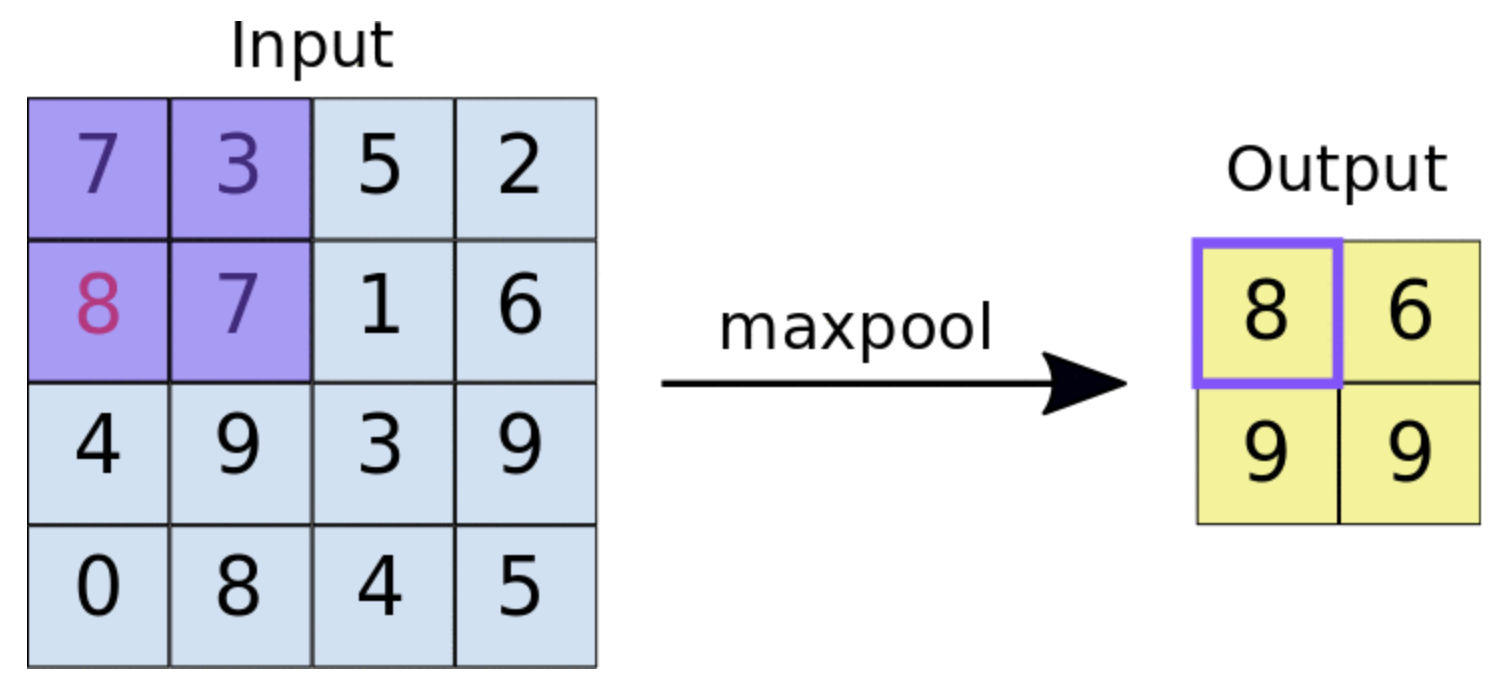
\includegraphics[scale=0.1]{maxpool.png}
    \caption{Example: maxpool}
    \label{}
\end{figure}\end{center}

\subsubsection{Unpooling}
\begin{definition}
    \underline{Unpooling} refers to the process of upsampling features by recreating the dimensions of feature map pooled and placing the pooled values into their original location.
\end{definition}
\begin{center}\begin{figure}[htbp]
    \centering
    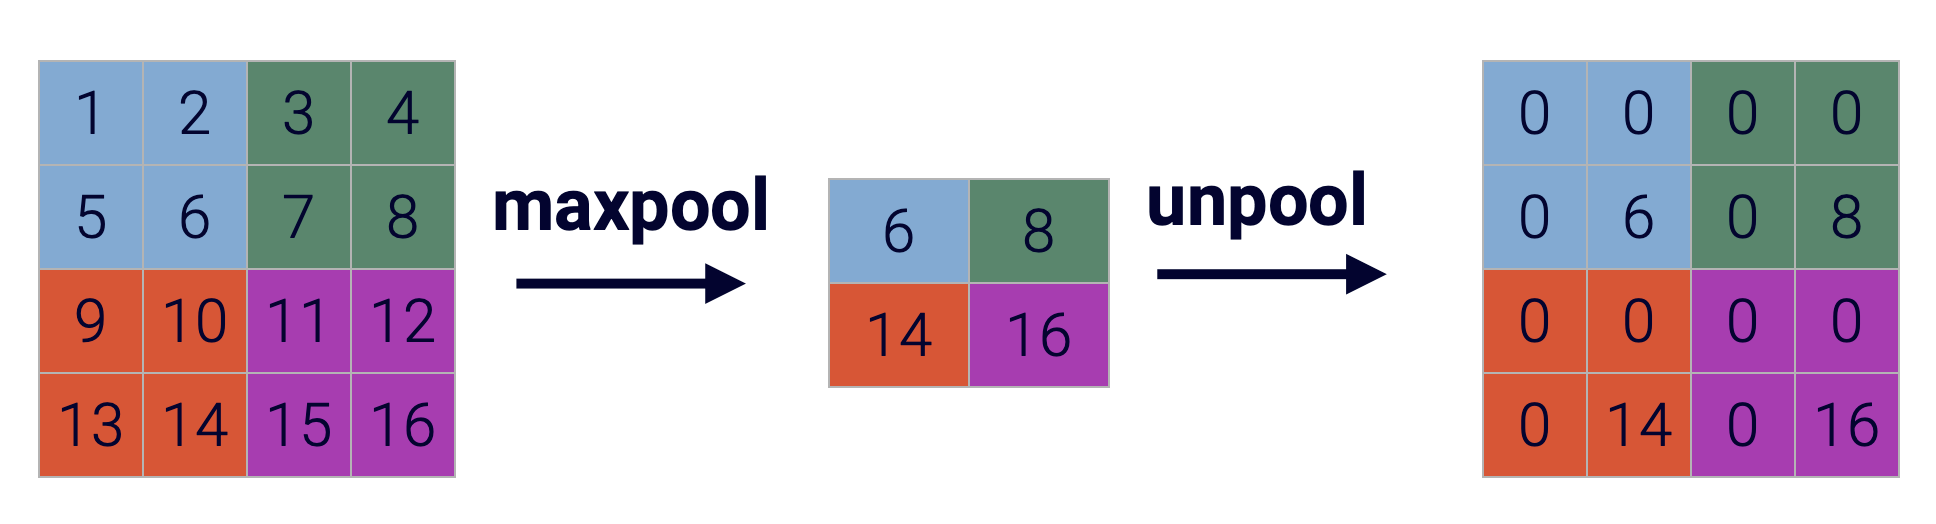
\includegraphics[scale=0.1]{unpool.png}
    \caption{Example: maxpool+unpool}
    \label{}
\end{figure}\end{center}



\section{Statistical Inference}

\subsection{Basics}
Given an observation $x\in X$, we want to estimate an unknown state $\theta \in S$ (not necessarily random). The $\theta$ can form $x$ with $P_\theta(x)$. We use decision rule $\delta (x)$ to form an action (estimation of $\theta$) $a=\hat{\theta}$.

\textbf{Example:}
\begin{enumerate}[(1)]
    \item Binary hypothesis testing (detection) when $S=\{0,1\}$ e.g. $P_0\sim N(0,\sigma^2), P_1\sim N(\mu,\sigma^2)$
    \item Multiple hypothesis testing (classification) when $S=\{1,2,...,n\}$
    \item (Estimation) when $S=\mathbb{R}$ e.g. $P_\theta\in N(\theta,\sigma^2)$
\end{enumerate}

\subsection{Decision Rule Examples}
\subsubsection*{Binary HT Example}
For the example Binary HT, $P_0\sim N(0,\sigma^2), P_1\sim N(\mu,\sigma^2)$: decision rule $\delta: \mathbb{R} \rightarrow \{0,1\}$

We can find a $\tau$ such that $\delta(x)=\left\{\begin{matrix}
    1,&x\ge \tau\\
    0,& else
\end{matrix}\right.=\mathbf{1}_{x\geq \tau}$. Howe to choose $\tau$?

Type-I error probability: probability that $\theta$ is $0$ but receive $\delta(x)=1$. $$P_I=P_0\{\delta(x)=1\}=P_0\{x\geq \tau\}=Q\left(\frac{\tau}{\sigma}\right)$$
Type-II error probability: probability that $\theta$ is $1$ but receive $\delta(x)=0$. $$P_{II}=P_1\{\delta(x)=0\}=P_1(x<\tau)=Q(\frac{\mu-\tau}{\sigma})$$

Both $P_I$ and $P_{II}$ depends on $\tau$. $Q(t)=\int_t^\infty\frac{e^{-\frac{x^2}{2}}}{\sqrt{2\pi}}dx$

For $\tau=\frac{\mu}{2}$, $P_I=P_{II}=Q\left(\frac{\mu}{2\sigma}\right)$

\subsubsection*{Multiple HT Example}
Consider three state $S=\{1,2,3\}$.
We can find a $\tau$ such that $\delta(x)=\left\{\begin{matrix}
    1,&x< \tau_1\\
    2,& \tau_1\leq x\leq \tau_2\\
    3,& x>\tau_2
\end{matrix}\right.=\mathbf{1}_{x\geq \tau}$.

\textit{Conditional Error Probabilities:} probability that $\theta$ is $i$ but receive $\delta(x)=j$ (6 types in this example) $$P_i\{\delta(x)=j\}, \forall i\neq j$$

\subsubsection*{Estimation Example}
Ex: $P_\theta\sim N(\theta,\sigma^2)$. Perform $\delta(x)=\hat{\theta}$ by using mean-squared error (MSE):
$$MSE= \mathbb{E}_\theta \left[(\delta(x)-\theta)^2\right],\theta\in \mathbb{R}$$

\subsection{Maximum-Likelihood Principle (state is norandom)}
Maximum-Likelihood Principle $$\hat{\theta}=\argmax_{\theta\in S}P_{\theta}(x)=\argmax_{\theta\in S}\ln P_{\theta}(x)$$
Applied to the binary example: $P_0\sim N(0,\sigma^2), P_1\sim N(\mu,\sigma^2)$.

$P_0(x)=\frac{1}{\sqrt{2\pi}\sigma}e^{-\frac{x^2}{2\sigma^2}}, P_1(x)=\frac{1}{\sqrt{2\pi}\sigma}e^{-\frac{(x-\mu)^2}{2\sigma^2}}$. $\ln P_0(x)=c-\frac{x^2}{2\sigma^2}$, $\ln P_1(x)=c-\frac{(x-\mu)^2}{2\sigma^2}$.

Then, the rule can become $$\hat{\theta}=\left\{\begin{matrix}
    0,&x^2<(x-\mu)^2\\
    1,&else
\end{matrix}\right.=\mathbf{1}_{x^2\geq (x-\mu)^2}=\mathbf{1}_{x\geq \frac{\mu}{2}}$$

\subsubsection*{Vector Observations}
Observations $X=\left(x_1,x_2,...,x_n\right)$, where i.i.d. $x_i\sim P_\theta$. Then $$P_\theta(X)=\prod_{i=1}^n P_\theta(x_i),\ \ln P_\theta(X)=\sum_{i=1}^n\ln P_\theta(x_i)$$
$\ln P_0(x)=cn-\frac{\sum_{i=1}^n x_i^2}{2\sigma^2}$, $\ln P_1(x)=cn-\frac{\sum_{i=1}^n(x_i-\mu)^2}{2\sigma^2}$.

Then, the rule can become $$\hat{\theta}=\left\{\begin{matrix}
    0,&\sum_{i=1}^nx_i^2<\sum_{i=1}^n(x_i-\mu)^2\\
    1,&else
\end{matrix}\right.=\mathbf{1}_{\sum_{i=1}^nx_i^2\geq \sum_{i=1}^n(x_i-\mu)^2}=\mathbf{1}_{\bar{x}\geq \frac{\mu}{2}}$$
where $\bar{x}=\frac{1}{n}\sum_{i=1}^nx_i$. Under both $H_0$ and $H_1$, $\bar{x}\sim N(0,\frac{\sigma^2}{n})$.

Then, type I error prob and type II error prob are the same $$P_I=P_0\{\bar{x}\geq \frac{\mu}{2}\}=P_{II}=P_1\{\bar{x}< \frac{\mu}{2}\}=Q\left(\frac{\mu\sqrt{n}}{2\sigma}\right)$$

\subsubsection*{Estimation $S=\mathbb{R}$}
To estimate $\theta$ when $S=\mathbb{R}$
\begin{equation}
    \begin{aligned}
        &\max_{\theta\in \mathbb{R}}\sum_{i=1}^n\ln P_\theta(x_i)\\
        &\Leftrightarrow \max_{\theta\in \mathbb{R}} \left[cn-\frac{\sum_{i=1}^n(x_i-\theta)^2}{2\sigma^2}\right]\\
        &\Leftrightarrow \max_{\theta\in \mathbb{R}} \sum_{i=1}^n(x_i-\theta)^2 \Rightarrow \hat{\theta}=\bar{x}
    \end{aligned}
    \nonumber
\end{equation}

Then, with $\bar{x}\sim N(\theta,\frac{\sigma^2}{n})$, the $$MSE_\theta=\mathbb{E}_\theta\left(\bar{x}-\theta\right)^2=\frac{\sigma^2}{n}$$

\subsection{Bayesian Decision Rule (state is random)}
\subsubsection{Rules}
Prior probability distribution $\pi(\theta)$,

\underline{Loss/cost function} with action (estimation) $a$ is $l(a,\theta)$. e.g.
\begin{enumerate}
    \item (binary HT) Hamming/zero-one loss $l(a=\hat{\theta},\theta)=\mathbf{1}_{a\neq \theta}$
    \item (estimation) Squared error loss $l(a=\hat{\theta},\theta)=(a-\theta)^2$; Absolute error loss $l(a,\theta)=|a-\theta|$.
\end{enumerate}

\textbf{Risk of decision rule $\delta$:} $$R(\delta)=\mathbb{E}\left(l(\delta(X),\theta)\right)$$ where $(X,\theta)$ are random with prob $\pi(\theta),P_\theta$

\textbf{Note: to help be consistent with machine learning notations, we use $y$ to substitute $\theta$.}

The joint probability $P(x,y)=\pi(y)P_y(x)=P(x)\pi(y|x)$.

\begin{example}
    The risk of decision $\delta(x)$ in Hamming/zero-one loss $l(a=\hat{y},y)=\mathbf{1}_{a\neq y}$
    \begin{equation}
        \begin{aligned}
            R(\delta)&=\mathbb{E}(\mathbf{1}_{\delta(x)\neq y})=\mathbb{E}[\delta(x)\neq y]\\
            &=P(y=0)P[\delta(x)\neq 0|y=0]+P(y=1)P[\delta(x)\neq 1|y=1]\\
            &=P(y=0)P[\delta(x)=1|y=0]+P(y=1)P[\delta(x)=0|y=1]
        \end{aligned}
        \nonumber
    \end{equation}
\end{example}

\textbf{Bayes rule}
$$\delta_B=\argmin_\delta R(\delta)$$
\underline{Derive Bayes rule}
\begin{equation}
    \begin{aligned}
        R(\delta)&=\int_x\int_y P(x,y) l(\delta(x),y) dy dx\\
        &=\int_x P(x)\int_y \pi(y|x) l(\delta(x),y) dy dx\\
    \end{aligned}
    \nonumber
\end{equation}
Solve optimization problem:
\begin{equation}
    \begin{aligned}
        \min_\delta \int_x P(x)\int_y \pi(y|x) l(\delta(x),y) dy dx
    \end{aligned}
    \nonumber
\end{equation}
\begin{center}
    \fcolorbox{black}{gray!10}{\parbox{.9\linewidth}{this problem can be transformed into optimization problems for each $x\in S$
    \begin{equation}
        \begin{aligned}
            \min_{\delta(x)} \int_y \pi(y|x) l(\delta(x),y) dy
        \end{aligned}
        \nonumber
    \end{equation}}}
\end{center}
\underline{The problem becomes to compute $\pi(y|x)$}. From $P(x,y)=\pi(y)P_y(x)=P(x)\pi(y|x)$, we know $$\pi(y|x)=\frac{\pi(y)P_y(x)}{P(x)}$$

\subsubsection{Maximum A Posteriori (MAP) Decision Rule (Binary example)}
\begin{example}
    Hamming/zero-one loss $l(a,y)=\mathbf{1}_{a\neq y}$
\end{example}

\textbf{Maximum A Posteriori (MAP) Decision Rule}:

Optimization problem is $$\delta(x)=\argmin_{a} \sum_{y=0,1} \pi(y|x) \mathbf{1}_{a\neq y} dy=\argmax_{y\in\{0,1\}}\pi(y|x)$$
$$\Rightarrow \sum_{y=0,1} \pi(y|x) \mathbf{1}_{\delta(x)\neq y} dx=\min_{a} \sum_{y=0,1} \pi(y|x) \mathbf{1}_{a\neq y} dy=\min\{\pi(1|x),\pi(0|x)\}$$

Likelihood ratio: $L(x)=\frac{P_1(x)}{P_0(x)}$

Likelihood ratio test: threshold $\tau=\frac{\pi(0)}{\pi(1)}$. If $L(x)>\tau$ accept $H_1$ (equivalent to $P_1(x)\pi(1)>P_0(x)\pi(0)$ which is also equivalent to comparing $\pi(y|x)$).

In this rule the whole optimization problem also goes to
\begin{equation}
    \begin{aligned}
        R(\delta_{MAP})&=\int_x P(x)\sum_{y=0,1} \pi(y|x) \mathbf{1}_{\delta(x)\neq y} dx\\
        &=\int_x P(x)\min\{\pi(1|x),\pi(0|x)\}dx
    \end{aligned}
    \nonumber
\end{equation}

\subsubsection{Minimum Mean Squared Error (MMSE) Rule ($\mathbb{R}^n$ example)}
\begin{example}
    (estimation) Squared error loss $l(a,y)=(a-y)^2$.
\end{example}
\subsubsection*{Minimum Mean Squared Error (MMSE) Rule:}
Optimization problem is $\delta(x)=\argmin_{a} \int_{y} \pi(y|x) (a-y)^2 dy$
\begin{equation}
    \begin{aligned}
        0=\int_{y} \pi(y|x) (\delta_B(x)-y) dy=\delta_B(x)-\mathbb{E}\left[Y|X=x\right]
    \end{aligned}
    \nonumber
\end{equation}
\begin{equation}
    \begin{aligned}
        \Rightarrow \delta_B(x)=\mathbb{E}\left[Y|X=x\right]
    \end{aligned}
    \nonumber
\end{equation}
which is called \textbf{conditional mean estimation}.

In this rule the whole optimization problem also goes to
$$R(\delta_{MMSE})=\int_x P(x)\int_y \pi(y|x) (y-\mathbb{E}\left[Y|X=x\right])^2 dy dx=\mathbb{E}_X Var\left[Y|X=x\right]$$

\textbf{Gaussian case:}
If $X\in \mathbb{R}^n$ and $(Y,X)$ are jointly Gaussian, then the conditional mean is a linear function of x, also called linear MMSE estimator.
\begin{equation}
    \begin{aligned}
        \mathbb{E}\left[Y|X=x\right]=\mathbb{E}[Y]+Cov(Y,X)Cov(X)^{-1}(x-\mathbb{E}[X])
    \end{aligned}
    \nonumber
\end{equation}
and the posterior risk is independent of $x$:
\begin{equation}
    \begin{aligned}
        Var\left[Y|X=x\right]=Var[Y]-Cov(Y,X)Cov(X)^{-1}Cov(X,Y)
    \end{aligned}
    \nonumber
\end{equation}
\subsection{Comparison}
Maximum-Likelihood Principle (state is norandom): $\delta_{ML}(x)=\argmax_y P_y(x)$.

Maximum A Posteriori (MAP) Decision Rule (state is random): $\delta_{MAP}(x)=\argmax_y \pi(y|x)=\argmax_y \{\pi(y|x),P_y(x)\}$


\section{Machine Learning in Inference}
Instead of given a prior distribution of $Y$, we are given a \textbf{training set} $T=(X_i,Y_i)_{i=1}^n$ where i.i.d. $(X_i,Y_i)\sim P$. (Distribution $P$ is unknown).

Risk: $R(\delta)=\mathbb{E}_P\left[l(\delta(X),Y)\right]$

The ture optimal decision rule is $$\delta_B=\argmin_\delta \mathbb{E}_P\left[l(\delta(X),Y)\right]$$
which is can't be computed since we don't know how actually $P$ is.

\subsection{Empirical Risk Minimization (ERM)}
Instead of computing optimal decision rule with $P$, we compute the optimal decisioin rule in the training set:
$$\hat{\delta}_n=\argmin_\delta \frac{1}{n}\sum_{i=1}^nl(\delta(X_i),Y_i)$$
The corresponding risk is $R(\hat{\delta}_n)=\mathbb{E}_P\left[l(\hat{\delta}_n(X),Y)\right]$. $\Delta R(\hat{\delta}_n)=R(\hat{\delta}_n)- R(\delta)>0$ always holds.

\textbf{Consistency:} if $\Delta R(\hat{\delta}_n) \rightarrow 0$ as $n \rightarrow \infty$.

\subsubsection{Example: Linear MMSE (LMMSE) estimator}
Use the decision role in the class of $\delta(x)=wx$. To find the linear MMSE (LMMSE) estimation $\delta^*(x)=w^*x$:
\begin{equation}
    \begin{aligned}
        w^*=\argmin_{w}\mathbb{E}_P\left[(wX-Y)^2\right]=\frac{\mathbb{E}[XY]}{\mathbb{E}[X^2]}
    \end{aligned}
    \nonumber
\end{equation}
The rule that minimizes the \textbf{empirical risk} is
\begin{equation}
    \begin{aligned}
        \hat{w}=\argmin_{w}\frac{1}{n}\sum_{i=1}^n(wX_i-Y_i)^2=\frac{\frac{1}{n}\sum_{i=1}^nX_iY_i}{\frac{1}{n}\sum_{i=1}^nX_i^2}
    \end{aligned}
    \nonumber
\end{equation}
The risk of the optimal rule $\delta^*=w^*x$ is $R(\delta^*)$ and the empirical risk under rule $\hat{\delta}(x)=\hat{w}x$ is $R(\hat{\delta}(x))$. $R(\hat{\delta})>R(\delta^*)$ always holds, and $$R(\hat{\delta})\rightarrow R(\delta^*)\text{ as }n \rightarrow \infty$$
According to CLT:
\begin{equation}
    \begin{aligned}
        \sqrt{n}\left(\frac{1}{n}\sum_iX_iY_i- \mathbb{E}(XY)\right) &\stackrel{d}{\longrightarrow} N(0,\sigma^2)\\
        \sqrt{n}\left(\frac{1}{n}\sum_iX_i^2- \mathbb{E}(X^2)\right) &\stackrel{d}{\longrightarrow} N(0,\sigma^2)
    \end{aligned}
    \nonumber
\end{equation}
Then,
\begin{equation}
    \begin{aligned}
        \frac{1}{n}\sum_iX_i^2=\mathbb{E}(X^2)+O(\frac{1}{\sqrt{n}})\\
        \frac{1}{n}\sum_iX_iY_i=\mathbb{E}(XY)+O(\frac{1}{\sqrt{n}})\\
    \end{aligned}
    \nonumber
\end{equation}
which means the error of estimators
\begin{equation}
    \begin{aligned}
        \hat{w}=\frac{\mathbb{E}(X^2)+O(\frac{1}{\sqrt{n}})}{\mathbb{E}(XY)+O(\frac{1}{\sqrt{n}})}=w^*+O(\frac{1}{\sqrt{n}})
    \end{aligned}
    \nonumber
\end{equation}
$$\hat{w}-w^*=O(\frac{1}{\sqrt{n}})$$
and the error of the risks:
\begin{equation}
    \begin{aligned}
        R(\hat{\delta})-R(\delta^*)&=\mathbb{E}_P[\hat{w}X-Y]^2-\mathbb{E}_P[w^*X-Y]^2\\
        &=\mathbb{E}_P[(\hat{w}-w^*)X+w^*X-Y]^2-\mathbb{E}_P[w^*X-Y]^2\\
        &=\mathbb{E}_P[(\hat{w}-w^*)X]^2+2(\hat{w}-w^*)\mathbb{E}_P[X(w^*X-Y)]\\
        &=(\hat{w}-w^*)\mathbb{E}_P(X^2)=O\left(\frac{1}{n}\right)
    \end{aligned}
    \nonumber
\end{equation}

\begin{center}
    \fcolorbox{black}{gray!10}{\parbox{.9\linewidth}{\textbf{\underline{Complexity}:}
    \begin{definition}
        A sequence $f(n)$ is $O(1)$ if $\lim_{n \rightarrow \infty}f(n)<\infty$.
    \end{definition}
    
    \begin{definition}
        A sequence $f(n)$ is $O(g(n))$ if $\frac{f(n)}{g(n)}$ is $O(1)$.
    \end{definition}
    
    \begin{definition}
        A sequence $f(n)$ is $o(1)$ if $\lim_{n \rightarrow \infty}\sup f(n)=0$.
    \end{definition}
    
    \begin{definition}
        A sequence $f(n)$ is $o(g(n))$ if $\lim_{n \rightarrow \infty}\sup \frac{f(n)}{g(n)}=0$.
    \end{definition}
    
    \begin{definition}
        A sequence $f(n)$ is \underline{asymptotic} to $g(n)$ if $\lim_{n \rightarrow \infty} \frac{f(n)}{g(n)}=1$. (This is denoted by $f(n)\sim g(n)$ as $a \rightarrow \infty$)
    \end{definition}
    }}
\end{center}

\subsubsection{Penalized ERM}
$\delta(x)=\sum_{j=1}^Jw_jx^j$

Pick $J=d$ and use ERM with $d$ dimensional $w$: $$\argmin_{w\in \mathbb{R}^d} \frac{1}{n}\sum_{i=1}^n[w^TX_i-Y_i]^2$$

Approach 1: Fix $d<<n$, use ERM.

Approach 2: (\textbf{Penalized ERM}) $$\min_\delta [R_{emp}(\delta)+J(\delta)]$$ ($J(\delta)$ is regularization (penalty) term)

\subsection{Stochastic Approximation}
Robbins and Monro (95)

\underline{Problem:} Find a root of function $h(x)$. ($f(x)=0$)

We do not observe $h(x)$ directly, but we observe $Y\sim P_x$ with
\begin{enumerate}[(1)]
    \item $\mathbb{E}[Y|X=x]=h(x)$
    \item $(Y|X=x)-h(x)$ is bounded
\end{enumerate}
\begin{example}
    $Y=X+Z$ with $\mathbb{E}[Z]=0$ and $Z$ is bounded.
\end{example}
Assumptions: 1. $h'(x^*)>0$; 2. $x^*$ is the unique root of $h$.

\textbf{SA Algorithm}
\begin{enumerate}[$\bullet$]
    \item Pick Sequence $\{a_n\}$ such that $\sum_{n=1}^\infty a_n=\infty$ and $\sum_{n=1}^\infty a^2_n<\infty$ (should converge to $0$ but not too quick) e.g. $a_n=n^{-\alpha}$ when $\alpha\in (\frac{1}{2},1]$.
    \item Initialize $X_1$
    \item Update for $n=1,2,...$, $Y_n\sim P(\cdot|X=X_n)$ $$X_{n+1}=X_n-a_n Y_n$$ until convergence.
\end{enumerate}

\begin{theorem}
    Under these assumptions $$X_n \stackrel{m.s.}{\longrightarrow} x^*\text{ as }n \rightarrow \infty$$ i.e., $\mathbb{E}(X_n-x^*)^2 \rightarrow 0$ as $n \rightarrow \infty$.
\end{theorem}

\begin{enumerate}[$\bullet$]
    \item \textbf{\underline{Performance Measure}} (Convergence rate): the root mean squared error (RMSE) $e_n=\sqrt{\mathbb{E}[(X_n-x^*)^2]}$.
    \item \underline{Projections}: If $x$ is constrained to live in an interval $I$, the update rule becomes $$X_{n+1}=\text{Proj}_x[X_n-a_nY_n]$$
    \item \underline{Averaging}: $$\bar{X}_n=\frac{1}{n}\sum_{i=1}^nX_i=\frac{X_n}{n}+\bar{X}_{n-1}\frac{n-1}{n}$$(nicer graph) (The benefits of this smoothing operation are mostly seen in the initial stages of the SA recursion, and \underline{do not improve the convergence rate}.)
\end{enumerate}

\begin{example}
    Let $h(x) = x$, in which case $x^* = 0$. $Y_n=h(X_n)+Z_n=X_n+Z_n$ where noise $Z_n$ is independent of $Y_n$ with $\mathbb{E}[Z_n]=0,Var(Z_n)=1$ and $Z_n$ is bounded.
\end{example}
Then,
    \begin{equation}
        \begin{aligned}
            X_{n+1}&=X_n-a_n(X_n+Z_n)\\
            &=(1-a_n)X_n-a_n Z_n
        \end{aligned}
        \nonumber
    \end{equation}
The MSE,
\begin{equation}
    \begin{aligned}
        e_{n+1}^2&=\mathbb{E}(X_{n+1}-x^*)^2=\mathbb{E}(X_{n+1})^2\\
        &=\mathbb{E}[(1-a_n)X_n-a_n Z_n]^2\\
        &=(1-a_n)^2\mathbb{E}X_n^2+a_n^2\mathbb{E}Z_n^2\\
        &=(1-a_n)^2e_n^2+a_n^2
    \end{aligned}
    \nonumber
\end{equation}
Pick $a_n=n^{-\alpha}$, where $\alpha\in (\frac{1}{2},1]$
\begin{equation}
    \begin{aligned}
        \Rightarrow e_{n+1}^2=(1-n^{-\alpha})^2e_n^2+n^{-2\alpha}
    \end{aligned}
    \nonumber
\end{equation}
\begin{center}
    \fcolorbox{black}{gray!10}{\parbox{.9\linewidth}{\center{Guess: $e_n=\sqrt{c}n^{-\beta}+H.O.T$}
    \begin{equation}
        \begin{aligned}
            c(n+1)^{-2\beta}+H.O.T=(1-n^{-\alpha})^2cn^{-2\beta}+n^{-2\alpha}+H.O.T
        \end{aligned}
        \nonumber
    \end{equation}
    (where $(n+1)^{-2\beta}=n^{-2\beta}(1+\frac{1}{n})^{-2\beta}=n^{-2\beta}[1-2\beta n^{^{-1}}+O(n^{-2})]$, by Taylor)
    \begin{equation}
        \begin{aligned}
            cn^{-2\beta}-2c\beta n^{^{-1-2\beta}}+H.O.T&=(1-n^{-\alpha})^2cn^{-2\beta}+n^{-2\alpha}+H.O.T\\
            -2c\beta n^{^{-1-2\beta}}+H.O.T&=-2cn^{-\alpha-2\beta}+n^{-2\alpha}+H.O.T
        \end{aligned}
        \nonumber
    \end{equation}
    \textbf{(For $\alpha<1$)}, $-2c\beta n^{^{-1-2\beta}}$ is not dominant term.
    $$H.O.T=-2cn^{-\alpha-2\beta}+n^{-2\alpha}+H.O.T$$
    Identify Power: $2\alpha=\alpha+2\beta$ $\Rightarrow$ $\beta=\frac{\alpha}{2}$ and $c=\frac{1}{2}$

    \textbf{(For $\alpha=1$)}, there are three dominant terms.
    $$-2c\beta n^{^{-1-2\beta}}+H.O.T=-2cn^{-1-2\beta}+n^{-2}+H.O.T$$
    Identify Power: $2=1+2\beta$ $\Rightarrow$ $\beta=\frac{1}{2}$ and $-2c\beta=-2c+1\Rightarrow c=1$

    $$e_n^2\sim c n^{-2\beta}$$
    To let the convergence rate as fast as possible, we want the $\beta$ to be as large as possible. Since $\beta=\frac{\alpha}{2}$, we pick the highest $\alpha=1 \Rightarrow \beta=\frac{1}{2},c=1$.
    $$e_n=O(n^{-\frac{1}{2}})\text{ with }a_n\sim\frac{1}{n}$$

    }}
\end{center}

\begin{example}
    Let $h(x) = x^3$, in which case $x^* = 0$. $Y_n=h(X_n)+Z_n=X_n^2+Z_n$ where noise $Z_n$ is independent of $Y_n$ with $\mathbb{E}[Z_n]=0,Var(Z_n)=1$ and $Z_n$ is bounded.
\end{example}
Then,
    \begin{equation}
        \begin{aligned}
            X_{n+1}&=X_n-a_n(X^3_n+Z_n)\\
            &=X_n-a_nX^3_n-a_n Z_n
        \end{aligned}
        \nonumber
    \end{equation}
Pick $a_n=n^{-\alpha}$, $\alpha\in (\frac{1}{2},1]$ $\Rightarrow \beta=\frac{1}{6},\alpha=\frac{2}{3}$ $\Rightarrow e_n\sim O(n^{-\frac{1}{6}})$

\subsection{Stochastic Gradient Descent (SGD)}
Solve $\min_{x\in\mathbb{R}^n}f(x)$.

We only use a \textbf{noisy version} $g(x,z)$ of $f(x)$, where $\mathbb{E}_z[g(x,z)]=f(x)$.
\begin{equation}
    \begin{aligned}
        \mathbb{E}_z[\nabla_x g(x,z)]=\nabla_x \mathbb{E}_z[g(x,z)]=\nabla f(x)
    \end{aligned}
    \nonumber
\end{equation}
Also pick sequence $\{a_n\}$ such that $\sum_{n=1}^\infty a_n=\infty$ and $\sum_{n=1}^\infty a^2_n<\infty$.

\textbf{SGD}
\begin{enumerate}[$\bullet$]
    \item Initialize $X_1$
    \item Update for $n=1,2,...$, $$X_{n+1}=X_n-a_n \nabla g(X_n,Z_n)$$
\end{enumerate}

\begin{example}
    $f(x)=\frac{1}{2}x^2,x\in \mathbb{R}$. Let $Z$ be a random variable with $\mathbb{E}(Z)=0,Var(Z)=1$. $$g(x,Z)=\frac{1}{2}(x+Z)^2-\frac{1}{2}$$
    \begin{equation}
        \begin{aligned}
            \mathbb{E}[g(x,Z)]&=\frac{1}{2}x^2=f(x)\\
            \nabla_x g(x,Z)&=x+Z \Rightarrow 
            \mathbb{E}[\nabla_xg(x,Z)]=\nabla f(x)
        \end{aligned}
        \nonumber
    \end{equation}
    $$X_{n+1}=X_n-a_n(X_n+Z_n)$$
    which is the same as the stochastic approximation.
\end{example}
\textbf{Main Results:} (Suppose the unique minimum is $x^*$)
\begin{enumerate}[(1)]
    \item \underline{Convergence:} $e_n \rightarrow 0$ as $n \rightarrow \infty$.
    \item \underline{Convergence Rate:} To achieve $\mathbb{E}[f(X_n)]-f(x^*)<\varepsilon$, we need $n=O(\frac{1}{\varepsilon})$ if $f$ is twice continuously differentiable and strongly convex.
\end{enumerate}

GD has linear convergence $\Rightarrow$ $e_n=O(e^{-cn})$; Solve $\varepsilon=O(e^{-cn}) \Rightarrow n=O(\ln \frac{1}{\varepsilon})$. (\textbf{SGD is much worse than GD}, cost more.)

\subsection{SGD Application to Empirical Risk Minimization (ERM)}
ERM problem is
$$\min_{w\in \mathbb{R}^d}\frac{1}{n}\sum_{i=1}^nL(\delta_w(X_i),Y_i)$$
$R_{emp}(w)=\frac{1}{n}\sum_{i=1}^nL(\delta_w(X_i),Y_i)$ is the empirical risk (e.g. $\delta_w(x)=w^Tx$, $L(\hat{y},y)=(\hat{y}-y)^2$)
To make $w$ more visible, we can write
\begin{equation}
    \begin{aligned}
        R_{emp}(w)=\frac{1}{n}\sum_{i=1}^nL(\delta_w(X_i),Y_i)
        =\frac{1}{n}\sum_{i=1}^nQ(X_i,Y_i,w)
    \end{aligned}
    \nonumber
\end{equation}
For penalized ERM we would similarly have $$\min_{w\in \mathbb{R}^d}\frac{1}{n}\sum_{i=1}^nQ(X_i,Y_i,w)+J(w)$$ $J(w)$ is the penalty (regularization) term.

In the problem $\min_{W\in \mathbb{R}^n}R_{emp}(w)=\frac{1}{n}\sum_{i=1}^nQ(X_i,Y_i,w)$

\subsubsection{Different Gradient Descent for ERM}
\begin{enumerate}
    \item[\textbf{GD}]
    \begin{enumerate}[$\bullet$]
        \item Initialize $W_1$
        \item Update for $k\geq 1$,
        Update: $W_{k+1}=W_k-a_k \frac{1}{n}\sum_{i=1}^n\nabla Q(X_i,Y_i,W_k)$
    \end{enumerate}
    \textbf{Computational cost:} The computational cost of GD is $O(dn)$ operations per iteration. Since GD has exponential convergence, the number of iterations needed to reach an optimization error of $\rho$ is $O(\log\frac{1}{\rho})$. Hence GD incurs a \underline{total computational cost of $O(dn\log\frac{1}{\rho})$} to reach a solution $W_k$ such that $R_{emp}(W_k)\leq \min_WR_{emp}(W)+\rho$
    \item[\textbf{SGD}]
    \begin{enumerate}[$\bullet$]
        \item Initialize $W_1$
        \item Update for $k\geq 1$,
        \begin{enumerate}[{Step} 1:]
            \item Pick $i$ uniformly over $\{1,...,n\}$
            \item $W_{k+1}=W_k-a_k \nabla Q(X_i,Y_i,W_k)$
        \end{enumerate}
    \end{enumerate}
    \textbf{Computational cost:} After $k$ iterations, $\mathbb{E}[R_{emp}(W_k)]\leq \min_W R_{emp}(W)+\rho$, for $k=O(\frac{1}{\rho})$ and $f$ twice differentiable and strongly convex. The cost per iteration is $O(d)$ (independent of $n$), so the \underline{total computational cost is $O(\frac{d}{\varepsilon})$}.
\end{enumerate}

\subsubsection{Constraints on Learning Problem}
\textbf{Why achieving a low value of $\rho$ is useful (low error of $R_{emp}(\cdot)$), since the cost function $R_{emp}(\cdot)$ is only a surrogate for the actual risk $R(\cdot)$?}


Typically, $d=O(n^b)$ where $0<b<1$.

For any numerical algorithm producing a decision rule $\tilde{\delta_n}$, the excess risk (compared to Bayes rule $\delta_B$) can be expressed as the sum of three terms:
\begin{equation}
    \begin{aligned}
        \Delta R(\tilde{\delta_n})&=R(\tilde{\delta_n})-R(\delta_B)\\&=[R(\tilde{\delta_n})-R(\hat{\delta_n})]+[R(\hat{\delta_n})-R(\delta^*)]+[R(\delta^*)-R(\delta_B)]
    \end{aligned}
    \nonumber
\end{equation}

where
\begin{equation}
    \begin{aligned}
        \delta_B&=\text{ Bayes rule}\\
        \delta^*&=\text{ best rule in } D=\argmin_{\delta\in D} R(\delta)\\
        \hat{\delta_n}&=\argmin_{\delta\in D}R_{emp}(\delta)\\
        \tilde{\delta_n}&=\text{solution of the algorithm after $k$ iterations}
    \end{aligned}
    \nonumber
\end{equation}
(Note: $D$ is the set of all available decision rule in approximation (e.g. all linear parameters $\{W,b\}$), which can't be better than Bayes rule)

The expected excess risk
\begin{equation}
    \begin{aligned}
        \epsilon =\mathbb{E}[\Delta R(\tilde{\delta_n})]=\underbrace{\mathbb{E}[R(\tilde{\delta_n})-R(\hat{\delta_n})]}_{\text{Comp. Error}=\rho}+\underbrace{\mathbb{E}[R(\hat{\delta_n})-R(\delta^*)]}_{\text{Est. Error}=O(\frac{d}{n})}+\underbrace{\mathbb{E}[R(\delta^*)-R(\delta_B)]}_{\text{Approx. Error}=O(d^{-\beta})}
    \end{aligned}
    \nonumber
\end{equation}

\textit{Estimation error} increases as $d$ increases, but \textit{approximation error} decreases as $d$ increases. To minimize the excess risk, we want to balance the last two items, that is $O(\frac{d}{n})=O(d^{-\beta})$: solve $$\frac{d}{n}=d^{-\beta} \Rightarrow d^{1+\beta}=n \Rightarrow d=n^{\frac{1}{1+\beta}}$$
$$\Rightarrow\text{ the last two items } O(\frac{d}{n})=O(d^{-\beta})=O(n^{-\gamma})$$
where $\gamma=\frac{\beta}{1+\beta}\in(0,1]$ is a constant.

To balance the three items, we want
\begin{center}
    $\rho=O(n^{-\gamma})\Rightarrow n=O(\rho^{-\frac{1}{\gamma}})$ and $d=O(n^{\frac{1}{1+\beta}})$
\end{center}

The update rule $W_{k+1}=W_k-a_k \nabla Q(X_k,Y_k,W_k)$, where $i\sim \text{Uniform}\{1,2,...,n\}$

\textbf{Relation to Online Learning:} When the training data are made available sequentially (instead of in a batch as assumed here), online learning can be used to sequentially learn the decision rules (or the weights that parameterize the decision rule).

\textbf{Variations on Basic SGD:} mini batch: replace $S$ by a subset $B$ and $n$ by $|B|$
$$\frac{1}{|B|}\sum_{i\in B}Q(X_i,Y_i,W_k)$$

\textbf{Averaging SGD:} $$\bar{W}_n=\frac{1}{n}\sum_{i=1}^nW_i=\frac{W_n}{n}+\bar{W}_{n-1}\frac{n-1}{n}$$

\textbf{SVRG (Stochastic Variance Randomed Gradient):} R. Johnson and T. Zhang, “Accelerating Stochastic Gradient Descent using Predictive Variance Reduction,” \textit{Proc. NIPS} 2013.

\textbf{Unsupervised learning:} If no explanatory variable $X$ is present, the problem reduces to
$$
\min _w \frac{1}{n} \sum_{i=1}^n Q\left(Y_i, w\right)
$$
which finds applications to various unsupervised learning problems. For instance the $k$-means clustering algorithm partitions $n$ data points $y_i, 1 \leq i \leq n$ in $\mathbb{R}^d$ into $k$ clusters with centroids $w_j, 1 \leq j \leq k$, in a way that minimizes the within-cluster sum-of-squares: WCSS $=\frac{1}{n} \sum_{i=1}^n \min _{1 \leq j \leq k}\left\|y_i-w_j\right\|^2$. Using the formalism of (7), we have $Q(y, w)=\min _{1 \leq j \leq k}\left\|y-w_j\right\|^2$ where $y \in \mathbb{R}^d$ and $w=\left\{w_j\right\}_{j=1}^k \in \mathbb{R}^{d \times k}$ is a matrix whose $k$ columns are the centroid vectors.


\section{Stachastic Integradtion Methods}
Integral $I=\int_Xf(x)dx$.

\subsection{Deterministic Methods (Better in Low Dimension)}
\subsubsection{Riemann Integration}
Riemann integral: approximation integral $I$ of $f(x)$ in $[a,b]$ with $$\hat{I}_n=\sum_{i=1}^n(\underbrace{x_i-x_{i-1}}_{\frac{b-a}{n}})f(x_i)$$
where $x_i=a+\frac{b-a}{n}i$. We can also denote $\hat{f}(x)=f(x_i)$ if $x\in (x_{i-1},x_i]$

The error $|\hat{I}_n-I|=\int_a^b|\hat{f}(x)-f(x)|dx$

Assume $f$ is differentiable and $\max_x|f'(x)|=c<\infty$, then $|\hat{f}(x)-f(x)|\leq \frac{b-a}{n}c$
$$\Rightarrow |\hat{I}_n-I|\leq \int_a^b\frac{b-a}{n}c\ dx=\frac{(b-a)^2}{n}c$$
That is $n\sim O\left(\varepsilon^{-1}\right)$

\subsubsection{Trapezoidal Rule}
Using average can be better. $$\hat{I}_n=\sum_{i=1}^n(\underbrace{x_i-x_{i-1}}_{\frac{b-a}{n}})\frac{f(x_i)+f(x_{i-1})}{2}$$
The upper bound of error is $|\hat{I}_n-I|\leq \frac{C}{n^2}$ for some constant $C$.

That is $n\sim O\left(\varepsilon^{-\frac{1}{2}}\right)$

\begin{center}\begin{figure}[htbp]
    \centering
    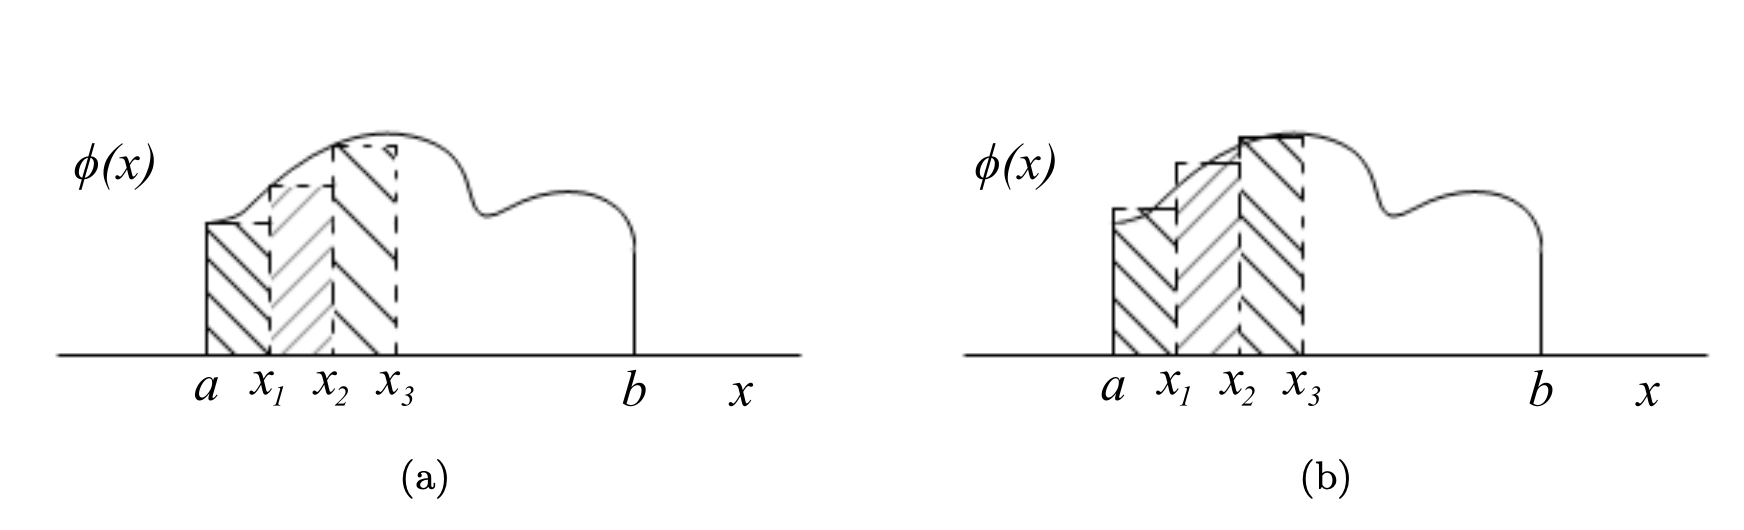
\includegraphics[scale=0.2]{Riemann and Trapezoidal.png}
    \caption{(a) Riemann approximation; (b) Trapezoidal approximation.}
    \label{}
\end{figure}\end{center}

\subsubsection{Multidimensional Integration}
When we want to do intergral in high dimention, it will be really hard.

For $d-$dimensional integrals, the trapezoidal rule yields an approximation error $|\hat{I}_n-I|\leq \frac{C}{n^\frac{2}{d}}$ for some constant $C$. That is $n\sim O\left(\varepsilon^{-\frac{d}{2}}\right)$. $n$ needs to increase exponentially with $d$ to achieve a target approximation error $\varepsilon$. This phenomenon is known as \underline{the curse of dimensionality}.
\begin{center}\begin{figure}[htbp]
    \centering
    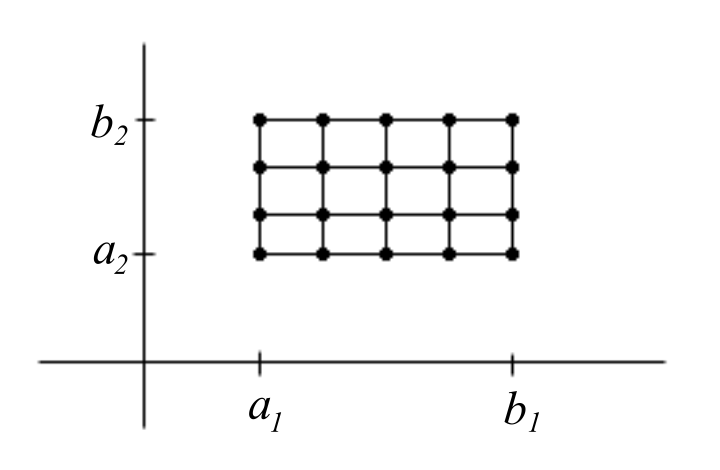
\includegraphics[scale=0.3]{two-dim int.png}
    \caption{Two-dimensional integration using regular grid.}
    \label{}
\end{figure}\end{center}



\subsection{Stachastic Methods (Better in High Dimension)}
\subsubsection{Classical Monte Carlo Integration}

Compute the expetation $$\xi=\mathbb{E}_p[h(x)]=\int_X \underbrace{p(x)h(x)}_{f(x)}dx$$

The methods described below can be used to solve the following problems: (1) General $\int_X f$; (2) Compute the probability of falling into a subset $a\subset X :P(a)=\int_a p(x)dx$, where $h(x)=\mathbf{1}_{x\in a}$

The Monte Carlo approach is as follows: Given $X_1, X_2, \cdots, X_n$ drawn i.i.d from the pdf
$p$, estimate $\xi $ by the empirical average $$\hat{\xi}_n=\frac{1}{n}\sum_{i=1}^nh(X_i)$$

$\mathbb{E}_p[\hat{\xi}_n]=\mathbb{E}_p[h(X)]=\xi$. $\hat{\xi}_n \stackrel{a.s.}{\longrightarrow}\xi$ as $n \rightarrow \infty$ by SLLW.

$Var(\hat{\xi}_n-\xi)=Var(\hat{\xi}_n)=\frac{1}{n}Var[h(x)]=O\left(\frac{1}{n}\right) \Rightarrow sd(\hat{\xi}_n)=\frac{\sqrt{Var[h(x)]}}{\sqrt{n}}$

That is $n\sim O\left(n^{-\frac{1}{2}}\right)$

The stochastic methods \textbf{outperform} when the deterministic ones for dimensions \underline{$d >4$} and are \textbf{worse} for \underline{$d<4$}.

\subsubsection{Importance Sampling}
Draw $X_i,i=1,...,n$ i.i.d from pdf $q$ $$\hat{\xi}_n=\frac{1}{n}\sum_{i=1}^n\frac{p(X_i)}{q(X_i)}h(X_i)$$
It is an unbiased estimator of $\xi$
\begin{equation}
    \begin{aligned}
        \mathbb{E}[\hat{\xi}_n]=\mathbb{E}_q[\frac{p(X_i)}{q(X_i)}h(X_i)]=\int_X p(x)h(x)dx=\xi
    \end{aligned}
    \nonumber
\end{equation}
$\hat{\xi}_n \stackrel{a.s.}{\longrightarrow}\xi$ as $n \rightarrow \infty$ by SLLW.

Its variance is
\begin{equation}
    \begin{aligned}
        {Var}_q(\hat{\xi}_n)&=\frac{1}{n}{Var}_q\left[\frac{p(X_i)}{q(X_i)}h(X_i)\right]\\
        &=\frac{1}{n}\left(\int_X\frac{p^2(x)}{q(x)}h^2(x)dx-\xi^2\right)
    \end{aligned}
    \nonumber
\end{equation}
The idea of importance sampling is to find a good $q$ such that $${Var}_q(\hat{\xi}_n)<{Var}_p(\hat{\xi}_n)$$

\subsubsection*{Error Meausre}
The \textit{relative error} of the importance-sampling estimator is defined as
$$
\delta_{\mathrm{rel}}\left(\hat{\xi}_n\right) \triangleq \frac{\sqrt{\operatorname{Var}_q\left(\hat{\xi}_n\right)}}{\xi}=\sqrt{\frac{\operatorname{Var}_q\left[\frac{p(X)}{q(X)} h(X)\right]}{\xi^2 n}} .
$$
The \textit{number} of simulations needed to achieve a relative error of $\delta$ is
$$
n_{I S}(\delta)=\frac{\operatorname{Var}_q\left[\frac{p(X)}{q(X)} h(X)\right]}{\xi^2 \delta^2} .
$$
The \textit{gain} \underline{relative to a Monte Carlo simulation} is defined as
$$
\Gamma=\frac{n_{M C}(\delta)}{n_{I S}(\delta)}=\frac{\operatorname{Var}_p[h(X)]}{\operatorname{Var}_q\left[\frac{p(X)}{q(X)} h(X)\right]}
$$

\textbf{In the example of $\xi=P(a), h(x)=\mathbf{1}_{x\in a}$:} Suppose $\xi=P(a)\approx 10^{-9}$ (small), $\hat{\xi}_n=\frac{1}{n}\sum_{i=1}^n\mathbf{1}_{X_i\in a}$. $\mathbf{1}_{X_i\in a}$ is $Bernoulli(\xi)$. We have $Var(\hat{\xi}_n)=\frac{\xi(1-\xi)}{n}$.

We can use relative error to measure $$\delta_{\mathrm{rel}}\left(\hat{\xi}_n\right)=\frac{\sqrt{Var(\hat{\xi}_n)}}{\xi}=\sqrt{\frac{1-\xi}{n\xi}}$$
and the number of simulation need to get relative error $\delta$ is $$
n_{I S}(\delta)=\frac{1-\delta} {\xi \delta^2} .
$$

\textbf{Find the optimal $q$:}
$$\min_q\int_X\frac{p^2(x)}{q(x)}h^2(x)dx-\xi^2$$
write $$\int_X\frac{p^2(x)}{q(x)}h^2(x)dx-\xi^2=\mathbb{E}_q\left[\left(\underbrace{\frac{p(x)}{q(x)}h(x)}_{Z}\right)^2\right]$$
Since $x^2$ is convex function, by Jensen's inequality
$$\mathbb{E}_q\left[\left(\underbrace{\frac{p(x)}{q(x)}h(x)}_{Z}\right)^2\right]\geq \left(\mathbb{E}_q\left[\underbrace{\frac{p(x)}{q(x)}h(x)}_{Z}\right]\right)^2$$
This equality holds if and only if $\frac{p(x)}{q(x)}h(x)=\alpha,\forall x\in X$, $\alpha$ is a constant.

Since $q$ is pdf., we can infer $$q(x)=\frac{p(x)h(x)}{\int_Xp(x)h(x)dx}$$
which is as hard as the original problem. In practice, one is content to find a “good” $q$ that assigns high probability to the important region where $p(x)h(x)$ is large. Ideally the ratio $\frac{p(x)}{q(x)}h(x)$ would be roughly constant over $X$.


\section{Bootstrap (not enough data)}
\underline{Problem:} analyze the performance of an estimator $\hat{\theta}_n(\vec{Y})$, $\vec{Y}=(Y_1,Y_2,...,Y_n)$ taken i.i.d. from distribution $P$. e.g. $P_{\theta}=N(0,1),\hat{\theta}_n=\frac{1}{n}\sum_{i=1}^nY_i$

Assume $\theta$ is a scalar parameter. Performance: (1) Bias $\mathbb{E}_{\theta}[\hat{\theta}_n(\vec{Y})]-\theta$; (2) Variance $\mathbb{E}_{\theta}[\hat{\theta}_n^2(\vec{Y})]-\mathbb{E}_{\theta}^2[\hat{\theta}_n(\vec{Y})]$; (3) CDF $G_{n}(t)=P(\hat{\theta}_n(\vec{Y})<t),\forall t$

\subsubsection*{Approach \#1 Monte-Carlo Simulations}
Generate $k$ vectors $\vec{Y}^{(i)},i=1,2,...,k$ (total $kn$ random variables)
(1) Bias $\frac{1}{k}\sum_{j=1}^k \hat{\theta}_n(\vec{Y}^{(j)})-\theta$; (2) Variance $\frac{1}{k}\sum_{j=1}^k \hat{\theta}^2_n(\vec{Y}^{(j)})-\left(\frac{1}{k}\sum_{j=1}^k \hat{\theta}_n(\vec{Y}^{(j)})\right)^2$; (3) CDF $\hat{G}_{n}(t)=\frac{1}{k}\sum_{j=1}^k \mathbf{1}_{\hat{\theta}_n(\vec{Y}^{(j)})<t},\forall t$

\subsubsection*{Approach \#2 Bootstrap}(When data is not enough)
Suppose we only have one data $\vec{Y}=(Y_1,...,Y_n)$

Reuse $Y_1,...Y_n$ to obtain resamples $\vec{Y}^*=(Y_1^*,...,Y_n^*)$. Do this $k$ times $\Rightarrow$ $k$ resamples ${\vec{Y^*}}^{(1)},...,{\vec{Y^*}}^{(k)}$

(1) Bias $\frac{1}{k}\sum_{j=1}^k \hat{\theta}_n(\vec{Y^*}^{(j)})-\theta$; (2) Variance $\frac{1}{k}\sum_{j=1}^k \hat{\theta}^2_n(\vec{Y^*}^{(j)})-\left(\frac{1}{k}\sum_{j=1}^k \hat{\theta}_n(\vec{Y^*}^{(j)})\right)^2$; (3) CDF $\hat{G}_{n}(t)=\frac{1}{k}\sum_{j=1}^k \mathbf{1}_{\hat{\theta}_n(\vec{Y^*}^{(j)})<t},\forall t$

\textbf{Example:} $\theta=med\{P\}$, $P$ is an unknown distribution over $\{0,1,...,9\}$. $\vec{Y}=(4,8,9,6,2)$.



\subsection{Residual Bootstrap}
The bootstrap principle is quite general and may also be used in problems where the data $Y_i$, $1\leq i\leq n$, \textbf{are not i.i.d}.

\subsubsection*{Example: Linear}
Observation $Y_i=a+b\frac{i}{n}+Z_i$, where $Z_i\sim N(0,\sigma^2)$ (i.i.d.) for $i=1,2,...,n$

Parameter $\theta=(a,b)$. Linear Least Square Estimator:
$$(\hat{a}_n,\hat{b}_n)=\argmin_{(a,b)}\sum_{i=1}^n(Y_i-a-b\frac{i}{n})^2$$
Given $\vec{Y}$, the residual (not i.i.d.)$$E_i=Y_i=\hat{a}_n-\hat{b}_n\frac{i}{n}\approx Z_i$$
Generate $k$ resamples of $\vec{E}=(E_1,E_2,...,E_n)$\\
$\Rightarrow$ obtain $\vec{E^*}^{(1)},\vec{E^*}^{(2)},...,\vec{E^*}^{(k)}$ by resampling\\
$\Rightarrow$ Compute pseudo-data ${Y_i^*}^{(j)}=\hat{a}_n+\hat{b}_n\frac{i}{n}+{E_i^*}^{(j)}$\\
$\Rightarrow$ Compute LS estimator $$\hat{\theta}_n^{(j)}=(\hat{a}_n^{(j)},\hat{b}_n^{(j)})=\argmin_{(a,b)}\sum_{i=1}^n({Y_i^*}^{(j)}-a-b\frac{i}{n})^2$$
$\Rightarrow$ Evaluate bias $$\widehat{Bias}=\frac{1}{k}\sum_{j=1}^k \hat{\theta}_n^{(j)}-\theta$$

\subsubsection*{Example: Nonlinear Markov Process}
Observation $Y_i=F_{\theta}(Y_{i-1})+Z_i$, where $Z_i\sim N(0,\sigma^2)$ (i.i.d.) for $i=1,2,...,n$

Parameter $\theta=(a,b)$. Linear Least Square Estimator:
$$\hat{\theta}_n(\vec{Y})=\argmin_{\theta}\sum_{i=1}^n(Y_i-F_{\theta}(Y_{i-1}))^2$$
Given $\vec{Y}$, the residual (not i.i.d.)$$E_i=Y_i=\hat{a}_n-F_{\hat{\theta}_n}(Y_{i-1})\approx Z_i$$
Generate $k$ resamples of $\vec{E}=(E_1,E_2,...,E_n)$\\
$\Rightarrow$ obtain $\vec{E^*}^{(1)},\vec{E^*}^{(2)},...,\vec{E^*}^{(k)}$ by resampling\\
$\Rightarrow$ Fix ${Y_0^*}^{(j)}=Y_0$, compute pseudo-data ${Y_i^*}^{(j)}=F_{\hat{\theta}_n}({Y^*_{i-1}}^{(j)})+{E_i^*}^{(j)}$\\
$\Rightarrow$ Compute LS estimator $$\hat{\theta}_n^{(j)}=\argmin_{(a,b)}\sum_{i=1}^n({Y_i^*}^{(j)}-F_{\hat{\theta}_n}({Y^*_{i-1}}^{(j)}))^2$$
$\Rightarrow$ Evaluate bias $$\widehat{Bias}=\frac{1}{k}\sum_{j=1}^k \hat{\theta}_n^{(j)}-\theta$$


\section{Particle Filtering}
Kalman filtering is used in tracking problems (dynamic models). Particle Filtering is an extension of Kalman filtering.
\subsection{Kalman Filtering}
\begin{enumerate}
    \item Unknown state sequence $X_t\in \mathbb{R}^m,t=0,1,2,...$
    \item Observations $Y_t\in \mathbb{R}^k,t=0,1,2,...$
    \item $X_{t+1}=F_tX_t+U_t$, $F_t\in \mathbb{R}^{m\times m}, U_t\sim P_{U_t}$
    \item $Y_t=H_tX_t+V_t$, $H_t\in \mathbb{R}^{k\times m}, V_t\sim P_{V_t}$
\end{enumerate}

We want to solve two problems
\begin{enumerate}
    \item \textbf{Estimation Problem:} Evaluate Linear MMSE (LMMSE) of $X_t$ given $Y_{0:t}$. $$\hat{X}_{t|t}=WY_{0:t}+b$$
    \item \textbf{Prediction Problem:} Predict Linear MMSE (LMMSE) of $X_{t+1|t}$ given $Y_{0:t}$. (Really hard)
\end{enumerate}

\subsection{Particle Filtering}
Particle filtering is a nonlinear form of Kalman filtering.

We consider a \underline{Nonlinear Dynamic System}
\begin{equation}
    \begin{aligned}
        X_{t+1}\sim q(\cdot|X_t)\\
        Y_{t}\sim r(\cdot|X_t)\\t=0,1,2,...
    \end{aligned}
    \nonumber
\end{equation}
where $q(X_{t+1}|X_t)$ is the transition probability distribution, and $r(Y_t|X_t)$ is the conditional probability distribution for the observations. Hence, $X_t$ is a Markov process and $Y_t$ follows a Hidden Markov Model (HMM).
\begin{center}\begin{figure}[htbp]
    \centering
    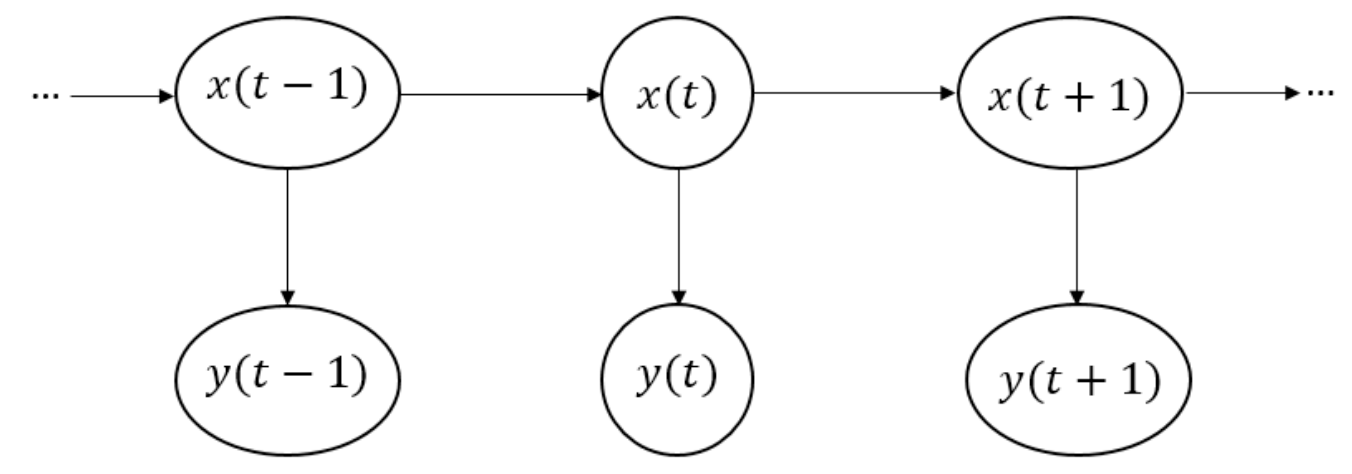
\includegraphics[scale=0.2]{HMM.png}
    \caption{Hidden Markov Model}
    \label{}
\end{figure}\end{center}
We also consider these two probelms.
\begin{enumerate}
    \item \textbf{Estimation Problem:} Evaluate $X_t$ given $Y_{0:t}$.
    \item \textbf{Prediction Problem:} Predict $X_{t+1|t}$ given $Y_{0:t}$.
\end{enumerate}

\subsubsection{Bayesian Recursive Filtering}
In this section we use Bayesian approach and use MMSE estimation $l(\hat{x}_t,x_t)=\|x_t-\hat{x}_t\|^2$

Estimation and prediction in conditional forms are:
\begin{equation}
    \begin{aligned}
        \hat{X}_{t|t}&=\mathbb{E}[X_{t}|Y_{0:t}]=\int_{\mathbb{R}^m}x_{t}P(X_{t}|Y_{0:t})dx_{t}\\
        \hat{X}_{t+1|t}&=\mathbb{E}[X_{t+1}|Y_{0:t}]=\int_{\mathbb{R}^m}x_{t+1}P(X_{t+1}|Y_{0:t})dx_{t+1}
    \end{aligned}
    \nonumber
\end{equation}

Apparently the posterior p.d.f cannot be evaluated due to the curse of dimensionality as $t$ increases. However, they can in principle be evaluated \textit{recursively} using the following two-step procedure.

\begin{enumerate}[\textbf{Step}]
    \item \textbf{ 1: Prediction.} $P(X_{t+1}|Y_{0:t})$ can be expressed in term of $P(X_t|Y_{0:t})$:
    \begin{equation}
        \begin{aligned}
            P(X_{t+1}|Y_{0:t})&=\int_{\mathbb{R}^m}P(X_{t+1},X_t|Y_{0:t})dx_t\\
            &=\int_{\mathbb{R}^m}P(X_{t+1}|X_t, Y_{0:t})P(X_t|Y_{0:t})dx_t\\
            &=\int_{\mathbb{R}^m}q(X_{t+1}|X_t)P(X_t|Y_{0:t})dx_t\\
        \end{aligned}
        \nonumber
    \end{equation}
    \item \textbf{ 2: Update.} We can also express $P(X_t|Y_{0:t})$ in terms of $P(X_t|Y_{0:t-1})$
    \begin{equation}
        \begin{aligned}
            P(X_{t}|Y_{0:t})&=P(X_t|Y_{t},Y_{0:t-1})\\
            &=\frac{P(Y_t|X_t,Y_{0:t-1})P(X_t|Y_{0:t-1})}{P(Y_t|Y_{0:t-1})}\\
            &=\frac{r(Y_t|X_t)P(X_t|Y_{0:t-1})}{\int_{\mathbb{R}^m}r(Y_t|X_t)P(X_t|Y_{0:t-1})dx_t}
        \end{aligned}
        \nonumber
    \end{equation}
\end{enumerate}

\subsubsection{Particle Filter (bootstrap filter)}
Suppose we have $n$ i.i.d. samples of $X_t$ drawn from $p(x_t|Y_{0:t})$: $X_t(1),X_t(2),...,X_t(n)$.
\begin{equation}
    \begin{aligned}
        X_{t}(i)\sim p(\cdot|Y_{0:t}),1\leq i\leq n
    \end{aligned}
    \tag{\text{Sample 1}}
\end{equation}

We can use above recursive filtering method to generate estimation of $X_{t+1}$.
\begin{enumerate}[\textbf{Step}]
    \item \textbf{ 1: Prediction.} Using the transition probability $q(\cdot|X_t(i)),1\leq i\leq n$ to generate $n$ independent random variables
    \begin{equation}
        \begin{aligned}
            X^*_{t+1}(i)\sim q(\cdot|X_t(i)),\ 1\leq i\leq n
        \end{aligned}
        \tag{\text{Sample 2}}
    \end{equation}
    \item \textbf{ 2: Update.} Upon receiving a new measurement $y_{t+1}$, evaluate the \textit{importance weights} (nonnegative and summing to $1$)
    \begin{equation}
        \begin{aligned}
            w_i=\frac{r(y_{t+1}|X_{t+1}^*(i))}{\sum_{j=1}^n r(y_{t+1}|X_{t+1}^*(j))},\ 1\leq i\leq n
        \end{aligned}
        \nonumber
    \end{equation}
    Then we resample $n$ times from the set $\{X_{t+1}^*(i)\}_{i=1}^n$ with respective probabilities $\{w_i\}_{i=1}^n$, obtaining i.i.d samples $\{X_{t+1}(j)\}_{j=1}^n$ with probabilities
    \begin{equation}
        \begin{aligned}
            Pr[X_{t+1}(j)=X_{t+1}^*(i)]=w_i,\ 1\leq i,j\leq n
        \end{aligned}
        \tag{\text{Sample 3}}
    \end{equation}
\end{enumerate}
By the \textbf{weighted bootstrap theorem}, as $n \rightarrow \infty$, the distribution of the
resampled $\{X_{t+1}(j)\}_{j=1}^n$ converges to the desired posterior.


Potential issues: 1. $n$ is not large enough. 2. Sample impoverishment





\section{EM Algorithm}

The ML estimator: $\hat{\theta}_{ML}=\argmax_{\theta\in S}\ln p_\theta(y)$. Numerical evaluation of maximum-likelihood (ML) estimates is often difficult. The likelihood function may have multiple extreme and the parameter $\theta$ may be multidimensional, all of which are problematic for any numerical algorithm.
\subsection{General Structure of the EM Algorithm}

\subsubsection*{What we want to estimate:}
$\theta\in S$ is an unknown parameter that we want to estimate.
\subsubsection*{What we know:}
\begin{enumerate}
    \item There is a complete data space $Z$ and an incomplete data space $Y$.
    \item The reality is $z\in Z$, which has p.d.f $q_{\theta}$. \textbf{Instead of observing the $z$ directly, we can observe $y=h(z)\in Y$ which has p.d.f $p_{\theta}$.}
    \item $h(z)=y$ is a many-to-one mapping.
    \item We can infer that the relationship between $q_\theta(z)$ and $p_\theta(y)$ is $$\sum_{z\in h^{-1}(y)}q_\theta(z)=p_\theta(y),\ \forall y$$
    \item For any function $f$, $\mathbb{E}_z[f(z)|y]$ depends on the p.d.f. $q_\theta$ and $p_\theta$. \begin{equation}
        \begin{aligned}
            \mathbb{E}_{z|\theta}[f(z)|y]=\sum_{z\in h^{-1}(y)}q_\theta(z|y)f(z)
        \end{aligned}
        \nonumber
    \end{equation}
\end{enumerate}
\begin{center}\begin{figure}[htbp]
    \centering
    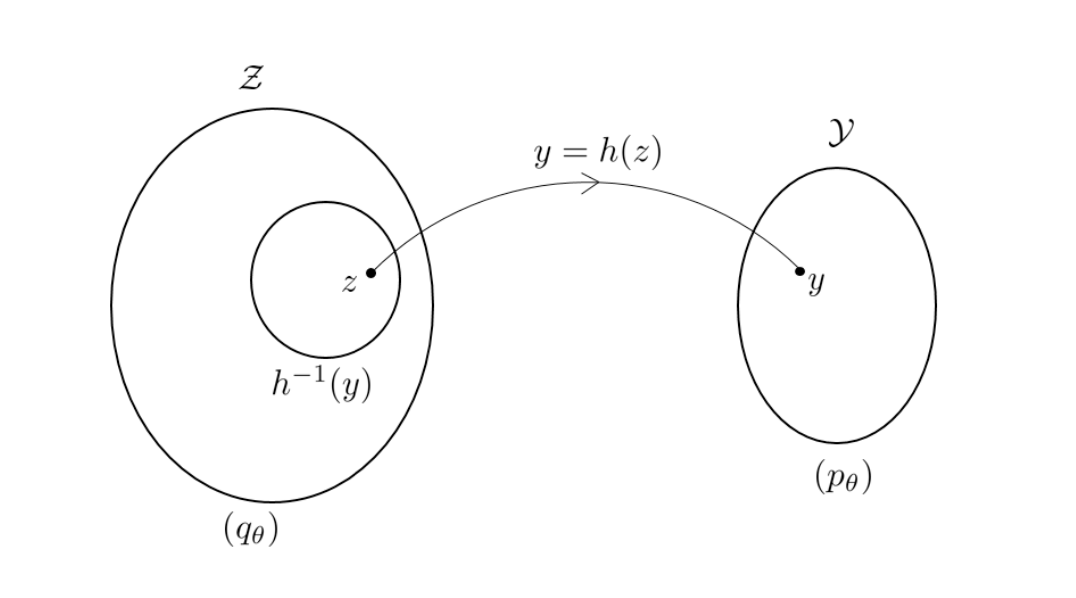
\includegraphics[scale=0.2]{EM1.png}
    \caption{Complete and incomplete data spaces $Z$ and $Y$.}
    \label{}
\end{figure}\end{center}

%The incomplete-data and complete-data loglikelihood functions are respectively denoted by
%\begin{equation}
%    \begin{aligned}
        %l_{id}(\theta)\triangleq \ln p_\theta(y);\ l_{cd}(\theta)\triangleq \ln q_\theta(z)
%    \end{aligned}
%    \nonumber
%\end{equation}
\subsubsection*{Maximum-Likelihood (ML) Estimation}
Given $y$, find the $\theta$ that maximizes $p_\theta(y)$
$$\hat{\theta}_{ML}=\argmax_{\theta\in S}\ln p_\theta(y)$$
\subsubsection*{EM Algorithm}
Instead of computing the $p_\theta(y)$ directly, we use the relationship $h(z)=y$ and $q_\theta(z)$ to estimate $\theta$.

EM algorithm alternates between Expectation (E) and Maximization (M) steps:
\begin{enumerate}
    \item Initialize $\hat{\theta}^{(0)}$
    \item For $k=0,1,2,...$\\
    \textbf{Expectation (E)-Step:}
        Compute
        \begin{equation}
            \begin{aligned}
                Q(\theta|\hat{\theta}^{(k)})
                &=\mathbb{E}_{z|\hat{\theta}^{(k)}}[\ln q_\theta(z)|Y=y]\\
                &=\sum_{z\in h^{-1}(y)}q_{\hat{\theta}^{(k)}}(z|y)\ln q_\theta(z)
            \end{aligned}
            \nonumber
        \end{equation}
    \textbf{Maximization (M)-Step} $$\hat{\theta}^{(k+1)}=\argmax_{\theta\in S}Q(\theta|\hat{\theta}^{(k)})$$
\end{enumerate}

\begin{definition}
    $\theta^*$ is a stable point of the EM algorithm if $\exists$ subsequence that converges to $\theta^*$.

    e.g. $1,3,\frac{1}{2},3,\frac{1}{3},3,...\frac{1}{n},3,...$
\end{definition}

\subsection{Example 1: Variance Estimation}
Observation $Y=S+N$, $S\sim \mathcal{N}(0,\theta)$ is independent of $N\sim \mathcal{N}(0,\theta)$ $\Rightarrow$ $Y\sim \mathcal{N}(0,\theta+1)$. $p_\theta(y)=\frac{1}{\sqrt{2\pi(\theta+1)}}e^{-\frac{y^2}{2(\theta+1)}}$. We want to estimate $\theta$.
\subsubsection{Maximum-Likelihood (ML) Estimation}
\begin{equation}
    \begin{aligned}
        \ln p_\theta(y)=-\frac{1}{2}\ln (2\pi)-\frac{1}{2}\ln(\theta+1)-\frac{y^2}{2(\theta+1)}
    \end{aligned}
    \nonumber
\end{equation}
take derivation of $\theta$ to be equal to $0$
\begin{equation}
    \begin{aligned}
        -\frac{1}{2(\theta+1)}+\frac{y^2}{2(\theta+1)^2}=0
    \end{aligned}
    \nonumber
\end{equation}
We can get $$\hat{\theta}=y^2-1$$
Then, $$\hat{\theta}_{ML}=\left\{\begin{matrix}
    0,&y^2\leq 1\\
    y^2-1,&y^2>1
\end{matrix}\right.$$

\subsubsection{EM Algorithm}
Let $Z=(S,N)$, $y=h(z)=s+n$.
\begin{equation}
    \begin{aligned}
        q_\theta(z)=q_\theta(s,n)=\frac{1}{\sqrt{2\pi\theta}}e^{-\frac{s^2}{2\theta}}\frac{1}{\sqrt{2\pi}}e^{-\frac{n^2}{2}}
    \end{aligned}
    \nonumber
\end{equation}
Then $$\ln q_\theta(z)=\ln \frac{1}{\sqrt{2\pi}}e^{-\frac{n^2}{2}}-\frac{1}{2}\ln (2\pi)-\frac{1}{2}\ln(\theta)-\frac{s^2}{2\theta}$$
\textbf{E-Step:}
        Compute
        \begin{equation}
            \begin{aligned}
                Q(\theta|\hat{\theta}^{(k)})
                &=\mathbb{E}_{z|\hat{\theta}^{(k)}}[\ln q_\theta(z)|Y=y]\\
                &=\sum_{z\in h^{-1}(y)}q_{\hat{\theta}^{(k)}}(z)\ln q_\theta(z)\\
                &=\ln \frac{1}{\sqrt{2\pi}}e^{-\frac{n^2}{2}}-\frac{1}{2}\ln (2\pi)-\frac{1}{2}\ln(\theta)-\frac{\mathbb{E}_{z|\hat{\theta}^{(k)}}(s^2)}{2\theta}
            \end{aligned}
            \nonumber
        \end{equation}
\textbf{M-Step}
\begin{equation}
    \begin{aligned}
        \hat{\theta}^{(k+1)}&=\argmax_{\theta\in S}Q(\theta|\hat{\theta}^{(k)})\\
        0&=-\frac{1}{2\hat{\theta}^{(k+1)}}+\frac{\mathbb{E}_{z|\hat{\theta}^{(k)}}(s^2)}{2(\hat{\theta}^{(k+1)})^2}\\
        \hat{\theta}^{(k+1)}&=\mathbb{E}_{z|\hat{\theta}^{(k)}}(s^2)=\frac{\hat{\theta}^{(k)}}{\hat{\theta}^{(k)}+1}\left(\frac{\hat{\theta}^{(k)}}{\hat{\theta}^{(k)}+1}y^2+1\right)
    \end{aligned}
    \nonumber
\end{equation}
Then we can solve the stable point
\begin{equation}
    \begin{aligned}
        \hat{\theta}^{*}=\frac{\hat{\theta}^{*}}{\hat{\theta}^{*}+1}\left(\frac{\hat{\theta}^{*}}{\hat{\theta}^{*}+1}y^2+1\right)\\
        \Rightarrow \hat{\theta}^{*}=0, \hat{\theta}^{*}=y^2-1
    \end{aligned}
    \nonumber
\end{equation}
According to the relation between $\hat{\theta}^{(k)}$ and $\hat{\theta}^{(k+1)}$, we can infer
$$\hat{\theta}^*=\left\{\begin{matrix}
    0,&y^2\leq 1\\
    y^2-1,&y^2>1
\end{matrix}\right.$$







\subsection{Example 2: Estimation of Gaussian Mixtures}
Assume the data $\boldsymbol{Y}=\left\{Y_i, 1 \leq i \leq n\right\} \in \mathbb{R}^n$, are drawn iid from a pdf $p_\theta(y)$ which is the mixture of $m$ univariate Gaussians with respective probabilities $\pi(j)$, means $\mu_j$, and variances $\sigma_j^2$, for $1 \leq j \leq m$ :
$$p_\theta(y|j)=\phi\left(y ; \mu_j, \sigma_j^2\right)$$
$$
p_\theta(y)=\sum_{j=1}^m \pi(j) \phi\left(y ; \mu_j, \sigma_j^2\right), \quad y \in \mathbb{R}
$$
where
$$\phi\left(y ; \mu, \sigma^2\right) \triangleq \frac{1}{\sqrt{2 \pi \sigma^2}} \exp \left\{-\frac{(y-\mu)^2}{2 \sigma^2}\right\}$$
denotes the Gaussian pdf with mean $\mu$ and variance $\sigma^2$.
\subsubsection{Unknown Means: ML estimation is hard}
We initially assume that $\{\pi(j)\}$ and $\left\{\sigma_j^2\right\}$ are given and that we only need to estimate the means $\left\{\mu_j\right\}$. Thus, $\theta=\mu \in \mathbb{R}^m$.

Unfortunately the ML estimator cannot be derived in closed form. Indeed, the loglikelihood function for $\theta$ is
$$
\ln \prod_{i=1}^n p_\theta(y_i)=\sum_{i=1}^n \ln p_\theta\left(y_i\right)=\sum_{i=1}^n \ln \sum_{j=1}^m \pi(j) \phi\left(y_i ; \mu_j, \sigma_j^2\right)
$$
and maximizing it is a $m$-dimensional, nonconcave maximization problem.

Taking the derivative of $\mu_j, j=1,...,m$,
\begin{equation}
    \begin{aligned}
        0&=\frac{1}{\sigma^2_j}\sum_{i=1}^n(y_i-\mu_j)\frac{\pi(j)\phi(y_i ; \mu_j, \sigma_j^2)}{\sum_{j=1}^m\pi(j)\phi(y_i ; \mu_j, \sigma_j^2)}\\
        &=\frac{1}{\sigma^2_j}\sum_{i=1}^n(y_i-\mu_j)\pi_\theta(j|y_i)
    \end{aligned}
    \nonumber
\end{equation}
where $\pi_\theta(j|y_i)\triangleq \frac{\pi(j)\phi(y_i ; \mu_j, \sigma_j^2)}{\sum_{j=1}^m\pi(j)\phi(y_i ; \mu_j, \sigma_j^2)}$.
The system may have multiple solutions corresponding to local maxima or even local minima or saddle points of the likelihood function.

\subsubsection{Unknown Means: EM Algorithm}

There is a complete data $Z_i=(J_i,Y_i),=1,...,n$, where $J_i$ is the random label that was drawn to produce $Y_i$. $z=\{j_i,y_i\}_{i=1}^n$ is the sample.
\begin{equation}
    \begin{aligned}
        q_\theta(z)&=\prod_{i=1}^n\left(\pi(j_i)p_\theta(y_i|j_i)\right)
    \end{aligned}
    \nonumber
\end{equation}
$$\ln q_{\theta}(z)=\sum_{i=1}^n[\ln \pi(j_i)+\ln p_{\theta}(y_i|j_i)]$$

Initialize $\hat{\theta}^{(0)}$

Iteration:
\begin{equation}
    \begin{aligned}
        Q(\theta|\hat{\theta}^{(k)})
        &=\sum_{i=1}^n\mathbb{E}_{\hat{\theta}^{(k)}}[\ln \pi(j_i)+\ln p_{\theta}(y_i|j_i)|Y_i=y_i]\\
        &=\sum_{i=1}^n\sum_{j=1}^m\pi_{\hat{\theta}^{(k)}}(j|y_i)[\ln \pi(j)+\ln p_{\theta}(y_i|j)]\\
        &=cst-\sum_{i=1}^n\sum_{j=1}^m\pi_{\hat{\theta}^{(k)}}(j|y_i)\frac{(y_i-\mu_j)^2}{2\sigma_j^2}\\
        &=cst-\sum_{i=1}^n\sum_{j=1}^m\frac{\pi(j)\phi(y_i ; \hat{\mu}_j^{(k)}, \sigma_j^2)}{\sum_{j=1}^m\pi(j)\phi(y_i ; \hat{\mu}_j^{(k)}, \sigma_j^2)}\frac{(y_i-\mu_j)^2}{2\sigma_j^2}
    \end{aligned}
    \nonumber
\end{equation}
where $\ln p_{\theta}(y_i|j)=-\frac{1}{2}\ln(2\pi\sigma_j^2)-\frac{(y_i-\mu_j)^2}{2\sigma_j^2}$.

Take derivative of $\mu_j$,
\begin{equation}
    \begin{aligned}
        0&=\frac{\partial Q(\theta|\hat{\theta}^{(k)})}{\partial \mu_j}=\sum_{i=1}^n\pi_{\hat{\theta}^{(k)}}(j|y_i)\frac{(y_i-\mu_j)}{\sigma_j^2}\\
        \hat{\mu}_j^{(k+1)}&=\frac{\sum_{i=1}^n\pi_{\hat{\theta}^{(k)}}(j|y_i)y_i}{\sum_{i=1}^n\pi_{\hat{\theta}^{(k)}}(j|y_i)}
    \end{aligned}
    \nonumber
\end{equation}

Recall the $\hat{\theta}_{ML}$
\begin{equation}
    \begin{aligned}
        \hat{\theta}_{ML,j}=\frac{\sum_{i=1}^n\pi_{\hat{\theta}_{ML}}(j|y_i)y_i}{\sum_{i=1}^n\pi_{\hat{\theta}_{ML}}(j|y_i)}
    \end{aligned}
    \nonumber
\end{equation}
$\hat{\theta}_{ML}$ is the stable point. (if exist)

\subsubsection{Unknown Mixture Probabilities, Means and Variances}
\textbf{ML Estimation:}

If $\theta \triangleq\left\{\pi(j), \mu_j, \sigma_j^2, 1 \leq j \leq m\right\}$ is unknown, the ML estimator $\hat{\theta}_{\mathrm{ML}}$ satisfies the following nonlinear system of equations:
$$
\begin{aligned}
\hat{\mu}_{\mathrm{ML}, j} &=\frac{\sum_{i=1}^n y_i \pi_{\hat{\theta}^{(k)}}\left(j \mid y_i\right)}{\sum_{i=1}^n \pi_{\hat{\theta}^{(k)}}\left(j \mid y_i\right)} \\
\hat{\sigma}_{\mathrm{ML}, j}^2 &=\frac{\sum_{i=1}^n\left(y_i-\hat{\mu}_{\mathrm{ML}, j}\right)^2 \pi_{\hat{\theta}^{(k)}}\left(j \mid y_i\right)}{\sum_{i=1}^n \pi_{\hat{\theta}(k)}\left(j \mid y_i\right)} \\
\hat{\pi}_{\mathrm{ML}}(j) &=\frac{1}{n} \sum_{i=1}^n \pi_{\hat{\theta}^{(k)}}\left(j \mid y_i\right) \quad 1 \leq j \leq m
\end{aligned}
$$
where
$$
\pi_\theta\left(j \mid y_i\right)=\frac{\pi(j) \phi\left(y_i ; \mu_j, \sigma_j^2\right)}{\sum_{j=1}^m \pi(j) \phi\left(y_i ; \mu_j, \sigma_j^2\right)}, \quad 1 \leq j \leq m
$$
\textbf{E-step:}
\begin{equation}
    \begin{aligned}
        Q(\theta|\hat{\theta}^{(k)})
        &=cst-\sum_{i=1}^n\sum_{j=1}^m\pi_{\hat{\theta}^{(k)}}(j|y_i)\frac{(y_i-\mu_j)^2}{2\sigma_j^2}\\
        &=cst-\sum_{i=1}^n\sum_{j=1}^m\frac{\hat{\pi}^{(k)}(j)\phi(y_i ; \hat{\mu}_j^{(k)}, \hat{\sigma_j^2}^{(k)})}{\sum_{j=1}^m\hat{\pi}^{(k)}(j)\phi(y_i ; \hat{\mu}_j^{(k)}, \hat{\sigma_j^2}^{(k)})}\frac{(y_i-\mu_j)^2}{2\sigma_j^2}
    \end{aligned}
    \nonumber
\end{equation}
\textbf{M-Step:}
\begin{equation}
    \begin{aligned}
        \hat{\mu}_j^{(k+1)} &=\frac{\sum_{i=1}^n y_i \pi_{\hat{\theta}^{(k)}}\left(j \mid y_i\right)}{\sum_{i=1}^n \pi_{\hat{\theta}(k)}\left(j \mid y_i\right)} \\
        \left(\hat{\sigma}_j^2\right)^{(k+1)} &=\frac{\sum_{i=1}^n\left(y_i-\hat{\mu}_j^{(k+1)}\right)^2 \pi_{\hat{\theta}^{(k)}}\left(j \mid y_i\right)}{\sum_{i=1}^n \pi_{\hat{\theta}^{(k)}}\left(j \mid y_i\right)} \\
        \hat{\pi}^{(k+1)}(j) &=\frac{1}{n} \sum_{i=1}^n \pi_{\hat{\theta}^{(k)}}\left(j \mid y_i\right), \quad 1 \leq j \leq m .
    \end{aligned}
    \nonumber
\end{equation}

\subsection{Information-Theoretic Functional}
\textbf{Definitions}
\begin{enumerate}
    \item \textbf{Entropy} of pmf $\{p(y),y\in Y\}$ $$H(p)=-\sum_{y\in Y}p(y)\ln p(y)$$
    (concave in $p$)
    \item \textbf{The Kullback-Leibler divergence (or relative entropy)} of two pmf's $p(x), x\in X$ and $q(x), x\in X$ is defined as
    \begin{equation}
        \begin{aligned}
            D(p\| q)=\sum_{y\in Y}p(y)\ln\frac{p(y)}{q(y)}\geq 0
        \end{aligned}
        \nonumber
    \end{equation}
    with equality iff $p=q$. (convex in $(p,q)$)
    \item \textbf{The cross-entropy} of a pmf $p(x),x\in X$ relative to another pmf $q(x), x\in X$
    \begin{equation}
        \begin{aligned}
            H(p, q)&=-\sum_{y\in Y}p(y)\ln q(y)\\&=H(p)+D(p\| q)
        \end{aligned}
        \nonumber
    \end{equation}
    $H(p,q)\geq H(p)$, the lower bound is achieved by $q=p$.
\end{enumerate}



\subsection{Convergence of EM Algorithm}
\begin{theorem}
    The likelihood sequence $p_{\hat{\theta}^{(k)}}(y)$, $k = 0, 1, 2, ...$ is nondecreasing.
\end{theorem}
\begin{proof}
    Assume for notational simplicity that the random variables $Y$ and $Z$ are discrete. Hence, their joint distribution is given by
    \begin{equation}
        \begin{aligned}
            P_\theta(y,z)&=q_\theta(z)p_\theta(y|z)=q_\theta(z)\mathbf{1}_{\{y=h(z)\}}\\
            &=p_\theta(y)q_\theta(z|y)
        \end{aligned}
        \nonumber
    \end{equation}
    Given $y$, the following identity holds for all $z \in h^{-1}(y)$:
    \begin{equation}
        \begin{aligned}
            p_\theta(y)&=\frac{q_\theta(z)}{q_\theta(z|y)}
        \end{aligned}
        \nonumber
    \end{equation}
    Taking the logarithm,
    \begin{equation}
        \begin{aligned}
            \ln p_\theta(y)&= \ln q_\theta(z)-\ln q_\theta(z|y),\ \forall z\in h^{-1}(y)
        \end{aligned}
        \nonumber
    \end{equation}
    Taking the conditional expectation with respect to $q_{\hat{\theta}}(z|y)$,
    \begin{equation}
        \begin{aligned}
            \ln p_\theta(y)&= \sum_{z\in h^{-1}(y)}q_{\hat{\theta}}(z|y)\ln q_\theta(z)-\sum_{z\in h^{-1}(y)}q_{\hat{\theta}}(z|y)\ln q_\theta(z|y)
        \end{aligned}
        \tag{1}
    \end{equation}
    \textbf{Expectation (E)-Step:}
        Compute
        \begin{equation}
            \begin{aligned}
                Q(\theta|\hat{\theta}^{(k)})
                &=\sum_{z\in h^{-1}(y)}q_{\hat{\theta}^{(k)}}(z|y)\ln q_\theta(z)
            \end{aligned}
            \nonumber
        \end{equation}
    \textbf{Maximization (M)-Step} $$\hat{\theta}^{(k+1)}=\argmax_{\theta\in S}Q(\theta|\hat{\theta}^{(k)})$$

    According to $(1)$,
    \begin{equation}
        \begin{aligned}
            \ln p_\theta (y)&=Q(\theta|\hat{\theta}^{(k)})-H(q_{\hat{\theta}^{(k)}},q_\theta)\\
            \ln p_{\hat{\theta}^{(k+1)}} (y)-\ln p_{\hat{\theta}^{(k)}} (y)&=(Q(\hat{\theta}^{(k+1)}|\hat{\theta}^{(k)})-Q(\hat{\theta}^{(k)}|\hat{\theta}^{(k)}))-(H(q_{\hat{\theta}^{(k)}},q_{\hat{\theta}^{(k+1)}})-H(q_{\hat{\theta}^{(k)}},q_{\hat{\theta}^{(k)}}))
        \end{aligned}
        \nonumber
    \end{equation}
    Since $\hat{\theta}^{(k+1)}=\argmax_{\theta\in S}Q(\theta|\hat{\theta}^{(k)})$, $Q(\hat{\theta}^{(k+1)}|\hat{\theta}^{(k)})-Q(\hat{\theta}^{(k)}|\hat{\theta}^{(k)})\geq 0$.
    \begin{equation}
        \begin{aligned}
            H(q_{\hat{\theta}^{(k)}},q_{\hat{\theta}^{(k+1)}})-H(q_{\hat{\theta}^{(k)}},q_{\hat{\theta}^{(k)}})=D(q_{\hat{\theta}^{(k)}}\| q_{\hat{\theta}^{(k+1)}})\geq 0
        \end{aligned}
        \nonumber
    \end{equation}
    Hence, we can conclude $\ln p_{\hat{\theta}^{(k+1)}} (y)-\ln p_{\hat{\theta}^{(k)}} (y)\geq 0$. Then $p_{\hat{\theta}^{(k)}}$ should be nondecreasing in $k$.
\end{proof}

\begin{corollary}
    Assume that $S$ is a closed, bounded subset of Euclidean space, the functions $Q(\theta|\theta')$ and $H(\theta|\theta')$ are continuously differentiable, and the loglikelihood function $\ln p_{\hat{\theta}^{(k)}}$ is differentiable and bounded. Then the sequence $\ln p_{\hat{\theta}^{(k)}}$ converges, and any limit point $\theta^*\in \text{interior}(S)$ of the EM sequence is a solution of the likelihood equation $\nabla \ln p_{\theta}=0$.
\end{corollary}


\subsection{EM As an Alternating Maximization Algorithm}
Define an \textit{auxiliary cost function} $L(q,\theta)$.

Incomplete data $Y$; Complete data $Z$. Still $h(z): Z \rightarrow Y$.

$\mathcal{Q}_y=\{q: q(z)=0, \forall z\in h^{-1}(y)\}$

\underline{EM updates}
\begin{enumerate}
    \item E-Step:
\end{enumerate}













\section{Hidden Markov model (HMM)}
A Markov chain ${X_t}_{t\geq 1}$ is observed as $\{Y_t\}_{t\geq 1}$. The state sets are finite sets $S_x, S_y$. Suppose the initial state distribution is $\pi$. The \textit{transition probability matrix} of the MC is
\begin{equation}
    \begin{aligned}
        A(i,j)=P(X_{t+1}=j|X_{t}=i),\ i,j\in S_x
    \end{aligned}
    \nonumber
\end{equation}
and the \textit{emission probability matrix} is
\begin{equation}
    \begin{aligned}
        B(i,j)=P(Y_t=j|X_t=i),\ i\in S_x, j\in S_y
    \end{aligned}
    \nonumber
\end{equation}
\begin{center}\begin{figure}[htbp]
    \centering
    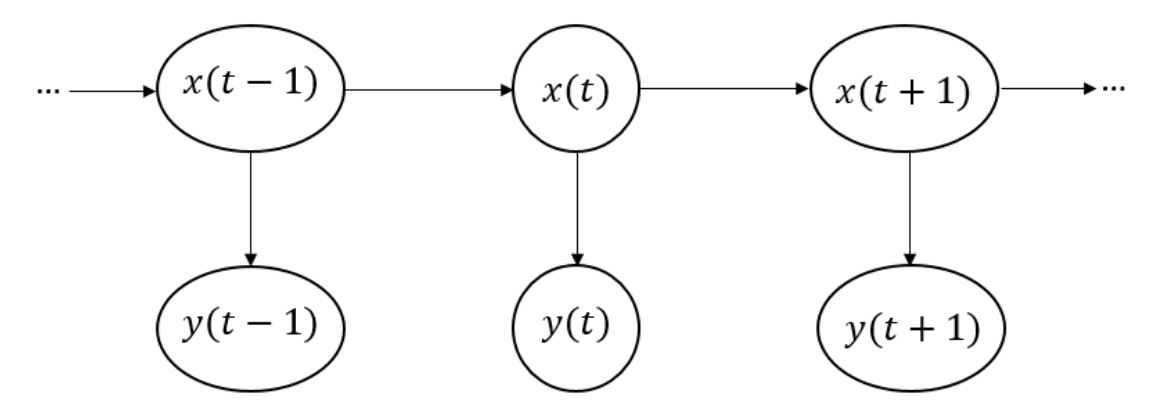
\includegraphics[scale=0.15]{HDM.png}
    \caption{Hidden Markov Model (HMM)}
    \label{}
\end{figure}\end{center}

Relative problems include
\begin{enumerate}[\textbf{Problem} 1:]
    \item Estimate $X_t$ given $Y_{1:t}$ (Using MAP or MMSE criterion: particle filtering)
    \item Estimate $X_{t+1}$ given $Y_{1:t}$ (Using MAP or MMSE prediction: particle filtering)
    \item Estimate $X_{1:t}$ given $Y_{1:t}$ (MAP, MMSE)
    \item Estimate the HMM parameters $\theta=(\pi,A,B)$ given $Y_{1:t}$ (learning)
\end{enumerate}

\subsection{Viterbi Algorithm: (MAP) estimate $X_{1:t}$ given $Y_{1:t}$}
\subsubsection{MAP estimation problem}
The MAP estimation problem arises in a variety of applications, and Viterbi derived a remarkable algorithm for solving it exactly. The probability of state $\vec{x}\in S_x^n$ is given by
\begin{equation}
    \begin{aligned}
        P(\vec{x})=\pi(x_1)\prod_{t=1}^{n-1}A(x_t,x_{t+1})
    \end{aligned}
    \nonumber
\end{equation}
and the conditional probability of the observed sequence $\vec{y}$ given the state sequence $\vec{x}$ is
\begin{equation}
    \begin{aligned}
        P(\vec{y}|\vec{x})=\prod_{t=1}^n B(x_t,y_t)
    \end{aligned}
    \nonumber
\end{equation}
Hence, the joint probability of $\vec{x}$ and $\vec{y}$ is
\begin{equation}
    \begin{aligned}
        P(\vec{x},\vec{y})=P(\vec{x})P(\vec{y}|\vec{x})=\pi(x_1)\prod_{t=1}^{n-1}A(x_t,x_{t+1})\prod_{t=1}^n B(x_t,y_t)
    \end{aligned}
    \nonumber
\end{equation}
Then the MAP estimation problem is
\begin{equation}
    \begin{aligned}
        \vec{x}^*&=\argmax_{\vec{x}}P(\vec{x}|\vec{y})=\argmax_{\vec{x}}\frac{P(\vec{x},\vec{y})}{P(\vec{y})}=\argmax_{\vec{x}}P(\vec{x},\vec{y})\\
        &=\argmax_{\vec{x}}\ \pi(x_1)\prod_{t=1}^{n-1}A(x_t,x_{t+1})\prod_{t=1}^n B(x_t,y_t)\\
        &=\argmax_{\vec{x}}\ \ln\pi(x_1)+\sum_{t=1}^{n-1}\ln A(x_t,x_{t+1})+\sum_{t=1}^n\ln B(x_t,y_t)
    \end{aligned}
    \nonumber
\end{equation}

\subsubsection{Viterbi Algorithm}
Let $f(x_1)=\ln\pi(x_1)+\ln B(x_1,y_1)$, $g_t(x_t,x_{t+1})=\ln A(x_t,x_{t+1})+\ln B(x_{t+1},y_{t+1})$. Then the estimation problem is written in the form
\begin{equation}
    \begin{aligned}
        \vec{x}^*=\argmax_{\vec{x}}\ \left[\varepsilon (\vec{x})=f(x_1)+\sum_{u=1}^{n-1}g_u(x_u,x_{u+1})\right]
    \end{aligned}
    \nonumber
\end{equation}
Let $V(1,x)=f(x)$ and
\begin{equation}
    \begin{aligned}
        V(t,x_t=x)\triangleq \max_{x_1,x_2,...,x_{t-1}}\left[\varepsilon([x_1,...,x_t])=f(x_1)+\sum_{u=1}^{t-1}g_u(x_u,x_{u+1})\right]
    \end{aligned}
    \nonumber
\end{equation}
\begin{equation}
    \begin{aligned}
        V(t,x_t=x)=\max_{x'} \left[V(t-1,x_{t-1}=x')+g_{t-1}(x',x)\right],\ t\geq 2
    \end{aligned}
    \nonumber
\end{equation}
Then, when $t=n$ we have
\begin{equation}
    \begin{aligned}
        \max_{\vec{x}}\varepsilon(\vec{x})=\max_{x} V(n,x_n=x)
    \end{aligned}
    \nonumber
\end{equation}

The complexity of the algorithm is $O(n|S_x|)$ storage and $O(n|S_x|^2)$ computation.

\begin{center}\begin{figure}[htbp]
    \centering
    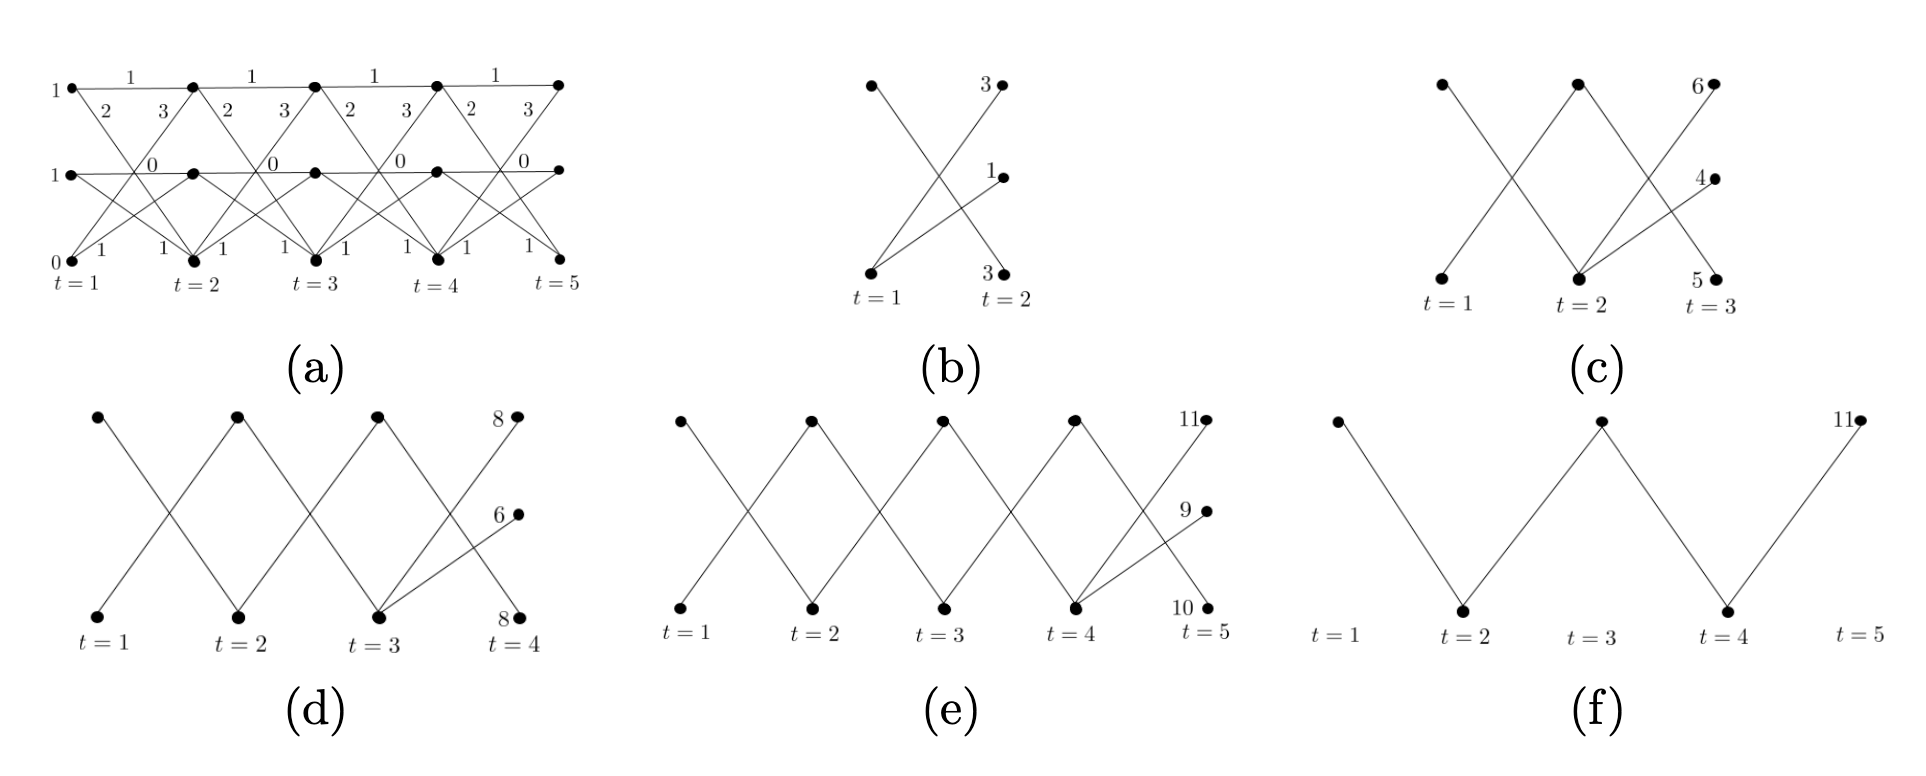
\includegraphics[scale=0.2]{dia.png}
    \caption{(a) Trellis diagram; (b)—(e) evolution of the Viterbi algorithm, showing surviving paths and values $V(t,x)$ at times $t = 2,3,4,5$; (f) optimal path $\vec{x}^* = (0,2,0,2,0)$ and its value $varepsilon(\vec{x}^*) = 11$.}
    \label{}
\end{figure}\end{center}


\section{Graphic Models}
\subsection{Graph Theory}
\begin{enumerate}
    \item A graph $(V,E)$, $V$ is a set of \textit{vertices}, $E\subseteq V\times V$ is a set of ordered pairs of vertices, called \textit{edges}.
    
    An edge $(i,j)\in E$ is \textit{directed} if $(i,j)\notin E$; otherwise the edge is \textit{undirected}. We denote directed and undirected edges by the symbols $i \rightarrow j$ and $i\sim j$, respectively.
    \item 
\end{enumerate}
\begin{center}\begin{figure}[htbp]
    \centering
    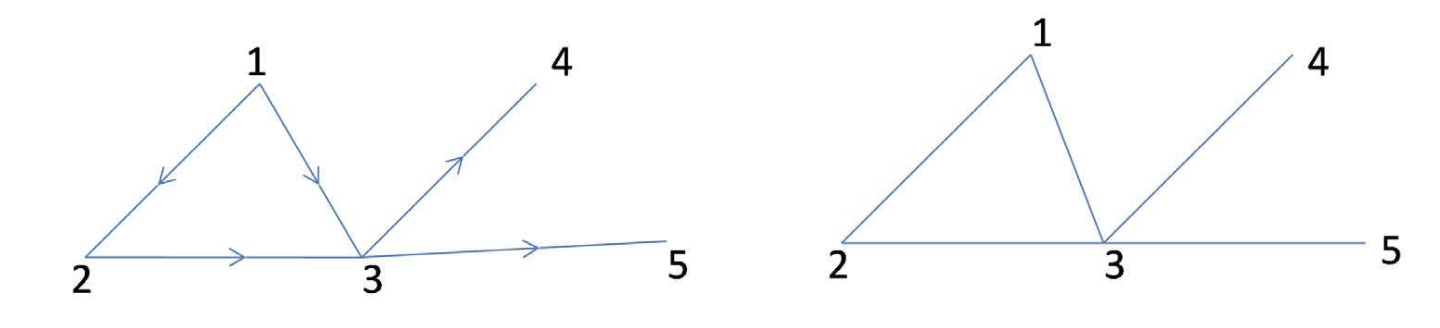
\includegraphics[scale=0.25]{graph.png}
    \caption{(a) Directed and (b) Undirected graph.}
    \label{}
\end{figure}\end{center}








































\end{document}